\documentclass[cjk,slidestop,compress,mathserif,blue]{beamer}
%dvipdfm选项是关键,否则编译统统通不过
%beamer的颜色选项定义的是导航条和标题的颜色(即关键词structure的颜色)

%%%%%%%%%%%%%%%%仅限于XeTeX可使用的宏包%%%%%%%%%%%%%%%%%%%%%%%%%%%%
\usepackage{fontspec,xunicode,xltxtra,beamerthemesplit}
%\usepackage{beamerthemesplit}
\usepackage{handoutWithNotes}		%(讲义)在打印PPT的时候会留出给每一页做注释的部分
\usepackage{xeCJK}
\setCJKmainfont[BoldFont=黑体, ItalicFont=楷体, BoldItalicFont=仿宋]{黑体}
%\setsansfont[Mapping=tex-text]{Adobe 黑体 Std}
%如果装了Adobe Acrobat,可在font.conf中配置Adobe字体的路径以使用其中文字体
%也可直接使用系统中的中文字体如SimSun,SimHei,微软雅黑 等
%原来beamer用的字体是sans family;注意Mapping的大小写,不能写错

\usepackage{listings} 
\lstset{language=Matlab}%代码语言使用的是matlab 
\lstset{breaklines}%自动将长的代码行换行排版 
\lstset{extendedchars=false}%解决代码跨页时,章节标\dots

%%%%%%%%   确定标题和导航条结构的框架     %%%%%%%%%%%%
\usepackage{beamerthemeshadow}                       %
%\usepackage{beamerthemeclassic}%导航条色与背景色一致%
%%%%%%%%%%%%%%%%%%%%%%%%%%%%%%%%%%%%%%%%%%%%%%%%%%%%%%
\setbeamerfont{roman title}{size={}}
%\usepackage{CJK} % CJK 中文支持                                  %
\usepackage{amsmath,amsthm,amsfonts,amssymb,bm}
\usepackage{mathrsfs}
\usepackage{xcolor}                                        %使用默认允许使用颜色
\usepackage{hyperref} 
\usepackage{graphicx}
\usepackage{subfigure}           %图片跨页
\usepackage{animate}		 %插入动画
\usepackage{caption}
\captionsetup{font=footnotesize}

\usepackage{multirow}

\usepackage[dvipdfmx]{movie15_dvipdfmx} %插入视频
%\usepackage{handoutWithNotes}		%(讲义)在打印PPT的时候会留出给每一页做注释的部分
%\pgfpagesuselayout{1 on 1 with notes landscape}[a4paper,border shrink=5mm]

%\usepackage[numbers,sort&compress]{natbib} %紧密排列             %
\usepackage[sectionbib]{chapterbib}        %每章节单独参考文献   %
\usepackage{hypernat}                                                                         %
%\usepackage[dvipdfm,bookmarksopen=true,pdfstartview=FitH,CJKbookmarks]{hyperref}		%
\hypersetup{bookmarksnumbered,colorlinks,linkcolor=brown,citecolor=blue,urlcolor=red}         %
%参考文献含有超链接引用时需要下列宏包,注意与natbib有冲突        %
%\usepackage[dvipdfm]{hyperref}                                  %
%\usepackage{hypernat}                                           %
\newcommand{\upcite}[1]{\hspace{0ex}\textsuperscript{\cite{#1}}} %

%\usepackage{marvosym} %插入各种符号

%\useoutertheme{smoothbars}
\useinnertheme[shadow=true]{rounded}
\usetheme{Berkeley}                                          %主题式样
%\usetheme{Luebeck}

\usecolortheme{lily}                                        %颜色主题式样

\usefonttheme{professionalfonts}                           %字体主题样式宏包

%\beamertemplatetransparentcoveredhigh                      %使所有被隐藏的文本高度透明
\beamertemplatetransparentcovereddynamicmedium             %使所有被隐藏的文本完全透明,动态,动态的范围很小
\mode<presentation>
%\beamersetaveragebackground{gray}                          %设置背景颜色(单一色) 
\beamertemplateshadingbackground{green!10}{red!5}         %设置背景颜色(渐变色)

%i放置单位logo
%\logo{
\includegraphics[width=1.6cm,height=0.35cm]{Figures/BCC_logo-1.png}}	%简单设置logo

%\pgfdeclareimage[width=3.5cm]{logoname}{Figures/BCC_logo-1.png}		%logo置于左侧微调
%\logo{\pgfuseimage{logoname}{\vspace{0.2cm}\hspace*{-2.0cm}}}

%在指定位置精确放置logo
\usepackage{tikz}
\usepackage{beamerfoils}
\usepackage{pgf}
\logo{\pgfputat{\pgfxy(11.68,0.15)}{
\includegraphics[height=1.01cm,viewport=0 0 140 120,clip]{Figures/BCC_logo-1.png}}\pgfputat{\pgfxy(10.502,-0.218)}{
\includegraphics[height=0.369cm,viewport=140 0 540 120,clip]{Figures/BCC_logo-1.png}}}
%\logo{\pgfputat{\pgfxy(11.68,0.15)}{
\includegraphics[height=0.95cm,viewport=0 0 510 360,clip]{Figures/Logo_Gainstrong.png}}\pgfputat{\pgfxy(10.333,-0.195)}{
\includegraphics[height=0.35cm,viewport=530 70 1100 218,clip]{Figures/Logo_Gainstrong.png}}}
%\logo{\pgfputat{\pgfxy(10.28,0.00)}{
\includegraphics[height=0.95cm,viewport=0 0 1100 360,clip]{Figures/Logo_Gainstrong.png}}}
%\logo{\pgfputat{\pgfxy(11.68,0.15)}{
\includegraphics[height=0.95cm,viewport=0 0 510 360,clip]{Figures/Logo_Gainstrong.png}}\pgfputat{\pgfxy(10.333,-0.195)}{
\includegraphics[height=0.35cm,viewport=530 70 1100 218,clip]{Figures/Logo_Gainstrong.png}}}
%\MyLogo{
%	\pgfputat{\pgfxy(-50,-50)}{\pgfbox[right,base]{
\includegraphics[height=1cm]{Figures/BCC_logo-1.png}}}

%logo作为背景放置
%\setbeamertemplate{background}{
%	\pgfputat{\pgfxy(6.5,-0.5)}{\pgfbox[left,top]{\pgfimage[height=1.1cm]{Figures/BCC_logo-1.png}}}}

%\logo{}									%不显示logo

\begin{document}
%\begin{CJK*}{GBK}{song}
%\begin{CJK*}{GBK}{kai}
%beamer下不能用\songyi、\zihao等命令!
%\graphicspath{Figures/}

%-------------------------------PPT Title-------------------------------------
\title{\rm{VASP}软件核心:~\rm{PAW}方法和迭代优化算法}
%-----------------------------------------------------------------------------

%----------------------------Author & Date------------------------------------
\author[\textrm{Jun\_Jiang}]{姜\;\;骏\inst{}} %[]{} (optional, use only with lots of authors)
% - Give the names in the same order as the appear in the paper.
% - Use the \inst{?} command only if the authors have different
%   affiliation.
\institute[BCC]{\inst{}%
 \vskip -30pt 北京市计算中心}
\date[\today] % (optional, should be abbreviation of conference name)
{	{\fontsize{6.2pt}{4.2pt}\selectfont{\textcolor{blue}{E-mail:~}\url{jiangjun@bcc.ac.cn}}}
\vskip 45 pt 2019.12.13
\vskip 5 pt {\fontsize{8.2pt}{6.2pt}\selectfont{山东大学}}}

% - Either use conference name or its abbreviation
% - Not really information to the audience, more for people (including
%   yourself) who are reading the slides online

\subject{}
% This is only inserted into the PDF information catalog. Can be left
% out.
\frame
{
%	\frametitle{\fontsize{9.5pt}{5.2pt}\selectfont{\textcolor{orange}{“高通量并发式材料计算算法与软件”年度检查}}}
\titlepage
}
%-----------------------------------------------------------------------------

%------------------------------------------------------------------------------列出全文 outline ---------------------------------------------------------------------------------
\section*{}
\frame[allowframebreaks]
{
  \frametitle{Outline}
%  \frametitle{\textcolor{mycolor}{\secname}}
  \tableofcontents%[current,currentsection,currentsubsection]
}
%在每个section之前列出全部Outline
%类似的在每个subsection之前列出全部Outline是\AtBeginSubsection[]
\AtBeginSection[]
{
  \frame<handout:0>
  {
    \frametitle{Outline}
%全部Outline中,本部分加亮
    \tableofcontents[current,currentsection]
  }
}

%------------------------------------------------------------------------------PPT main Body------------------------------------------------------------------------------------
\small
\section{材料计算的理论基石}       %Bookmark
\frame
{
%	\frametitle{\textrm{DFT-SCF}}
\begin{figure}[h!]
\vspace*{-0.25in}
\centering
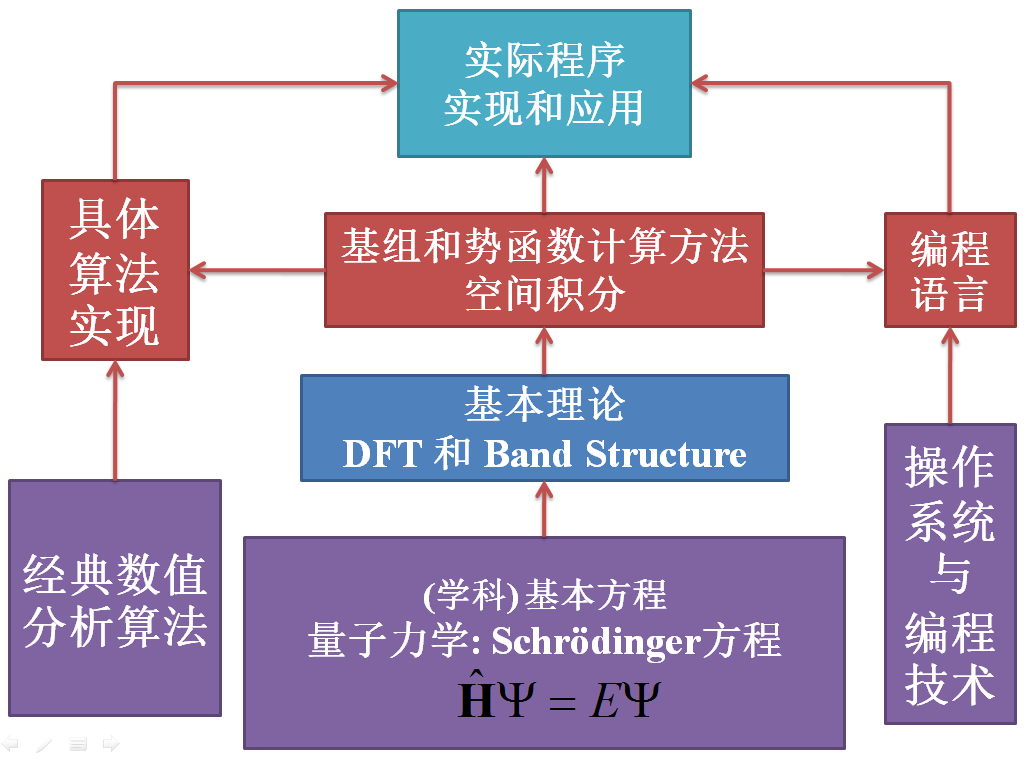
\includegraphics[height=2.80in,width=4.95in,viewport=5 3 1250 780,clip]{Figures/Method_Procedure.png}
%\caption{\small \textrm{Pseudopotential for metallic sodium, based on the empty core model and screened by the Thomas-Fermi dielectric function.}}%(与文献\cite{EPJB33-47_2003}图1对比)
\label{Method-Procedure}
\end{figure}
}

\subsection{密度泛函理论}       %Bookmark
\frame                               %
{
\frametitle{密度泛函理论} %Slide Page Title
%   \secname
\begin{itemize}%[+-| alert@+>]
	\item 密度泛函理论(\textrm{Density Functional Theory, DFT}):~通过体系的电子密度而非波函数确定体系的基态能量。
		密度泛函理论的基石:\textrm{Hohenberg-Kohn}定理\upcite{PR136-B864_1964}
\begin{itemize}%[+-| alert@+>]
	\item \textrm{\small{第一定理:~多电子体系的性质完全由体系的基态密度决定}}
   	\item \textrm{\small{第二定理:~基态总能量泛函在体系基态电子密度处取极小值}}
   \end{itemize}
%\textrm{\small{第二定理指出基态总能量泛函在体系基态电子密度处取极小值}}
 \item 密度泛函理论的优点:用密度($\rho$)代替波函数($\Psi$)描述体系
 \item 密度泛函理论的困难:能量密度泛函的精确形式未知
   \end{itemize}
\textrm{Kohn-Sham}方程\upcite{PR140-A1133_1965}:~无相互作用体系+交换-相关能
$$(T_S+V_{e\!f\!f})|\varphi_i\rangle=\varepsilon_i|\varphi_i\rangle,\quad i=1,\cdots,N,\cdots$$
其中$V_{e\!f\!f}(\vec r)=v(\vec r)+\displaystyle\int w(\vec r,\vec r\,')\rho(\vec r\,')\mathrm{d}\vec r+\dfrac{\delta E_{XC}}{\delta\rho(\vec r)}$
%\textrm{Kohn-Sham}方程是形式上的单粒子方程
%\textrm{Kohn-Sham}方程的
\\实质:~\textcolor{red}{将动能泛函的主要部分分离出来,剩余部分放在交换-相关能中}
}
%  \beamertemplateshadingbackground{blue!10}{yellow!10}
\subsection{固体能带理论}       %Bookmark
\frame
{
%\frametitle{The Bloch theorem}
	\frametitle{固体能带理论}
\begin{itemize}%[+-| alert@+>]
   \setlength{\itemsep}{8pt}
   \item 固体能带理论\upcite{Huang_Han}是固体电子理论的基础,形式上是单电子理论:
    $$\hat H |\psi_i^{\vec k}(\vec r)\rangle=\bigg[-\dfrac{\hbar^2}{2m}\nabla^2+V(\vec r)\bigg]|\psi_i^{\vec k}(\vec r)\rangle=\epsilon_i(\vec k)|\psi_i^{\vec k}(\vec r)\rangle$$
  \item \textrm{Bloch}定理:
%   \item \textrm{periodic potential:} $$V(\vec r)=V(\vec r+\vec R_n)$$
%     \textrm{Here,} $\vec R_n=n\vec R$
%   \item \textrm{Bloch theorem:}$$\psi_{\vec k}(\vec r)=\textrm{e}^{\textrm i\vec k\cdot\vec r}u_{\vec k}(\vec r)$$
%     \textrm{Here, $u_{\vec k}(\vec r)$ is a periodic function with the same periodicity as $V(\vec r)$, i.e., $u_{\vec k}(\vec r)=u_{\vec k}(\vec r+\vec R_n)$, then Bloch theorem could reads as:}
%     $$\psi_{\vec k}(\vec r+\vec R_n)=\textrm{e}^{\textrm i\vec k\cdot\vec R_n}\psi_{\vec k}(\vec r)$$
具有平移周期性的理想晶体,势能$V(\vec r)$满足$$V(\vec r)=V(\vec r+\vec R_n)$$
体系的波函数满足\textrm{Bloch}波函数形式:$$\psi_{\vec k}(\vec r)=\textrm{e}^{i\vec k\cdot\vec r}u_{\vec k}(\vec r)$$
是平面波和周期函数的乘积。$u(\vec r)$与势能有相同的周期。即$$u_{\vec k}(\vec r)=u_{\vec k}(\vec r+\vec R_n)$$
  \item 能带理论相当于分子轨道理论
%   \setlength{\itemsep}{30pt}
\item \textrm{Bloch}函数反映了波函数在周期性势场下的变化规律。
\end{itemize}
}

\frame
{
\frametitle{自由电子气模型}
简并态微扰理论引起的能带裂分
\begin{figure}[h!]
\centering
%\hspace*{-10pt}
%\vspace*{-1.1in}
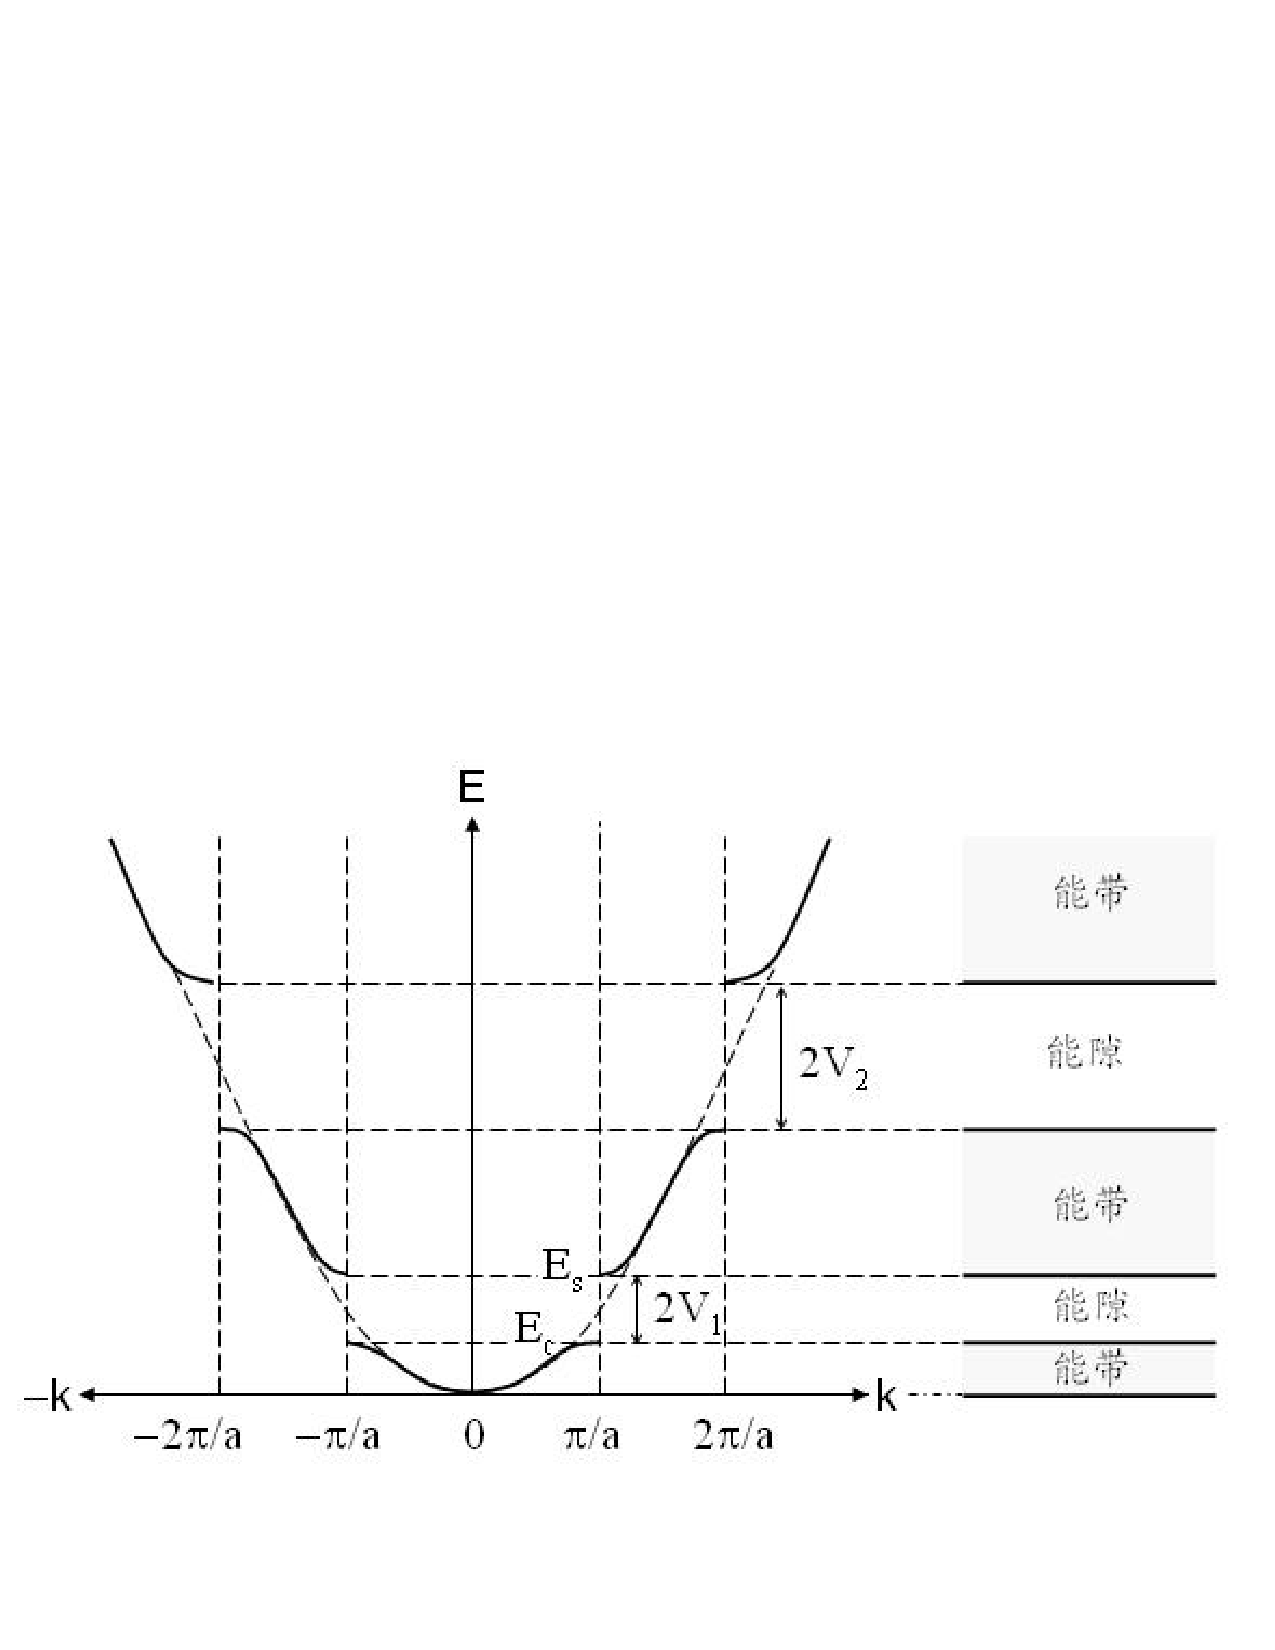
\includegraphics[height=2.1in,width=3.8in,viewport=10 90 570 380,clip]{Figures/Band_Gap.pdf}
\caption{\small \textrm{The Band-structure from free-electron gas.}}%
\label{Band-Structure-1}
\end{figure} 
}

\frame
{
\frametitle{紧束缚模型}
从分子轨道到能带
\begin{figure}[h!]
\centering
\hspace*{-0.29in}
\vspace*{-0.1in}
\subfigure[一维$\mathrm{H}$原子链]{
\label{fig:Hydrogen-1D}
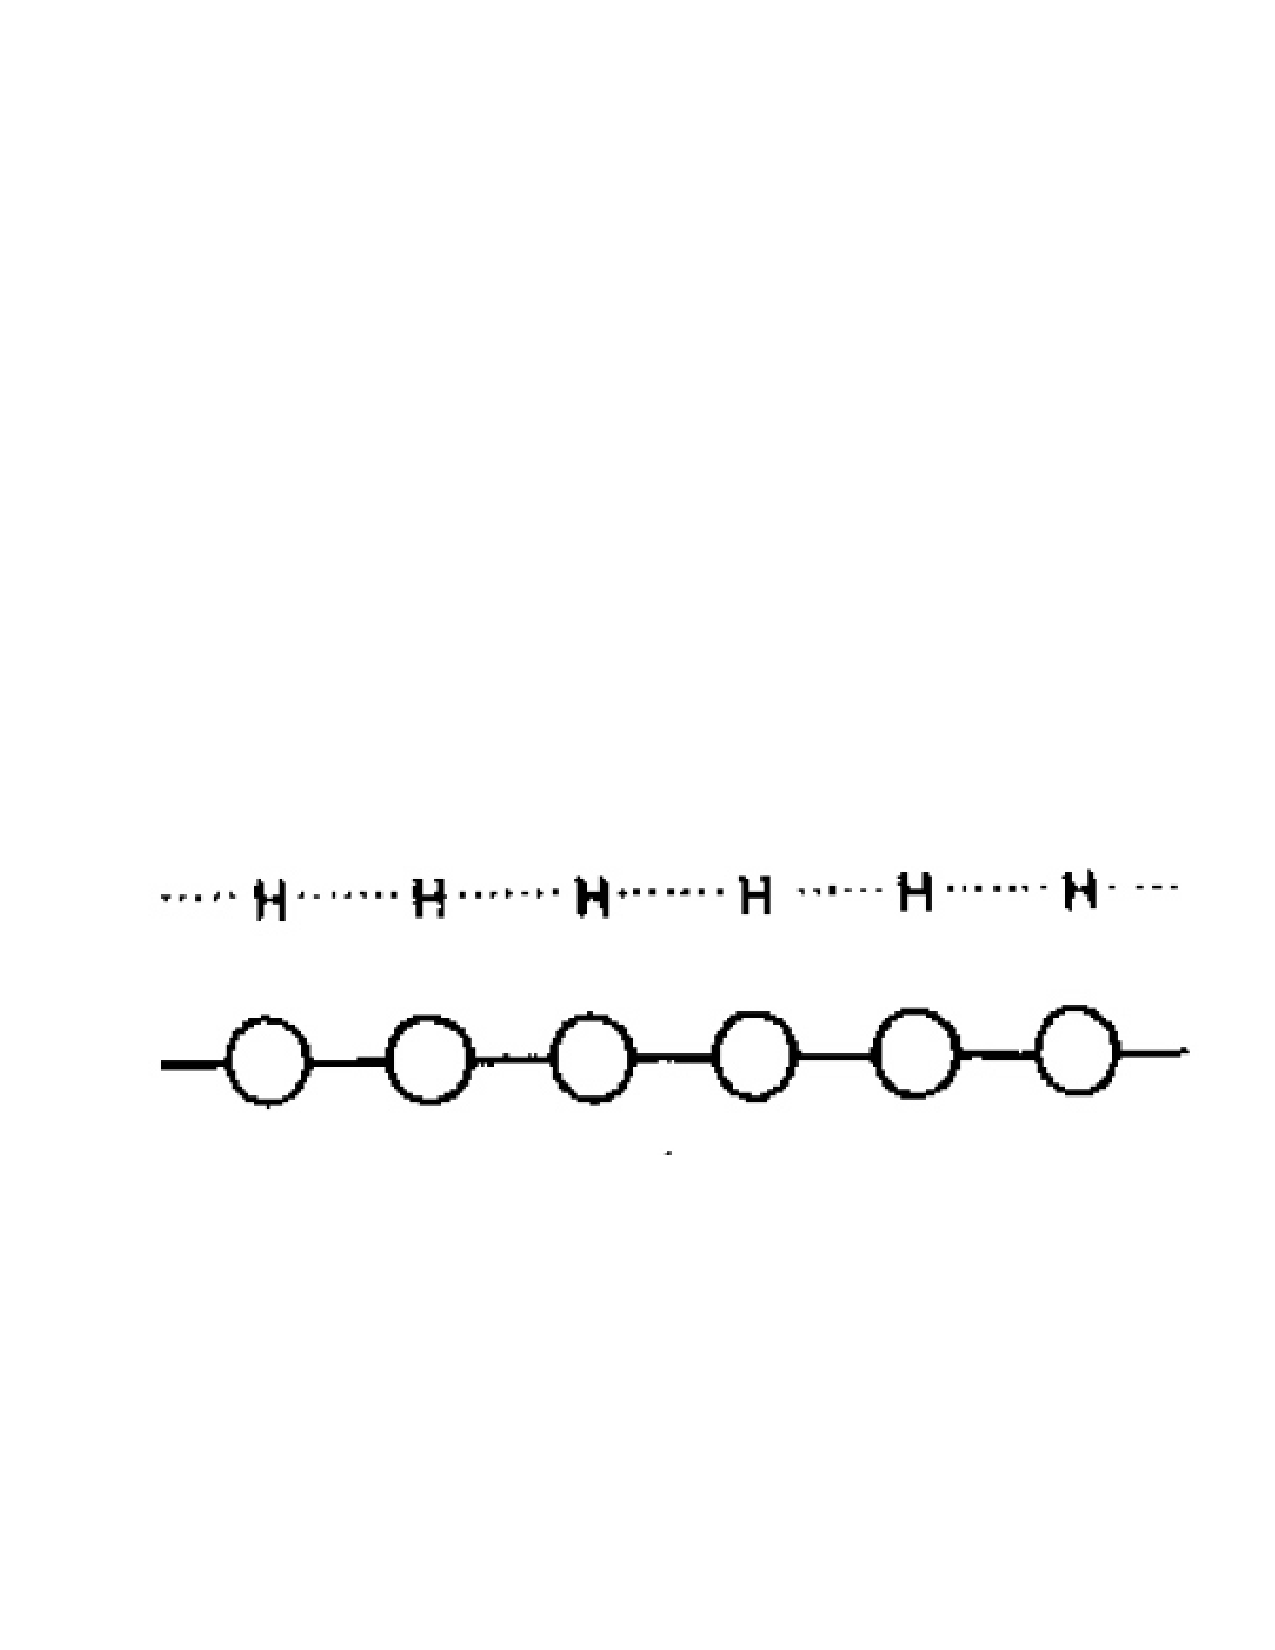
\includegraphics[height=0.25in,width=1.1in,viewport=70 255 570 375,clip]{Figures/Hydrogen-1D.pdf}}
\subfigure[$\mathrm{H}_n$分子轨道]{
\label{fig:Hydrogen-2-n}
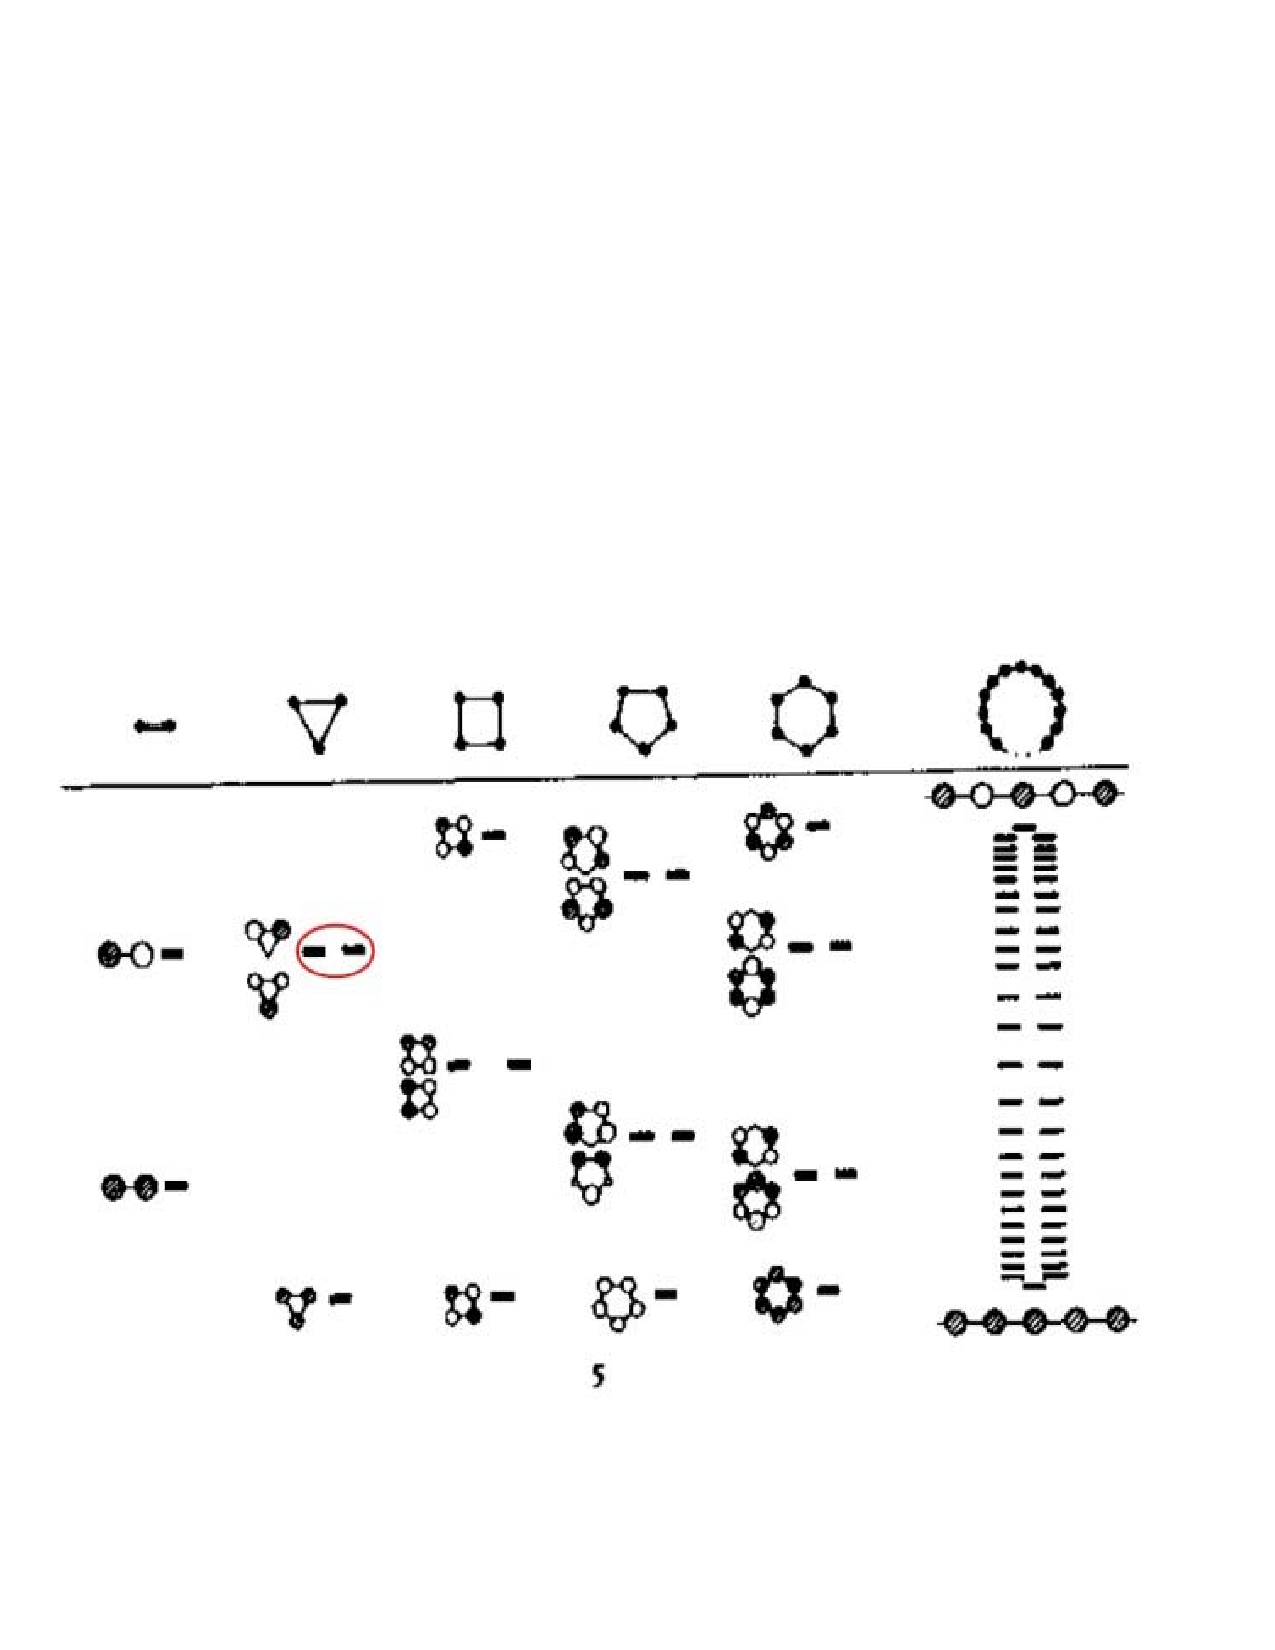
\includegraphics[height=0.8in,width=1.5in,viewport=30 140 545 480,clip]{Figures/Hydrogen-Mol-Orbital.pdf}}
\subfigure[分子波函数]{
\label{fig:Hydrogen-Psi}
\vspace*{-0.2in}
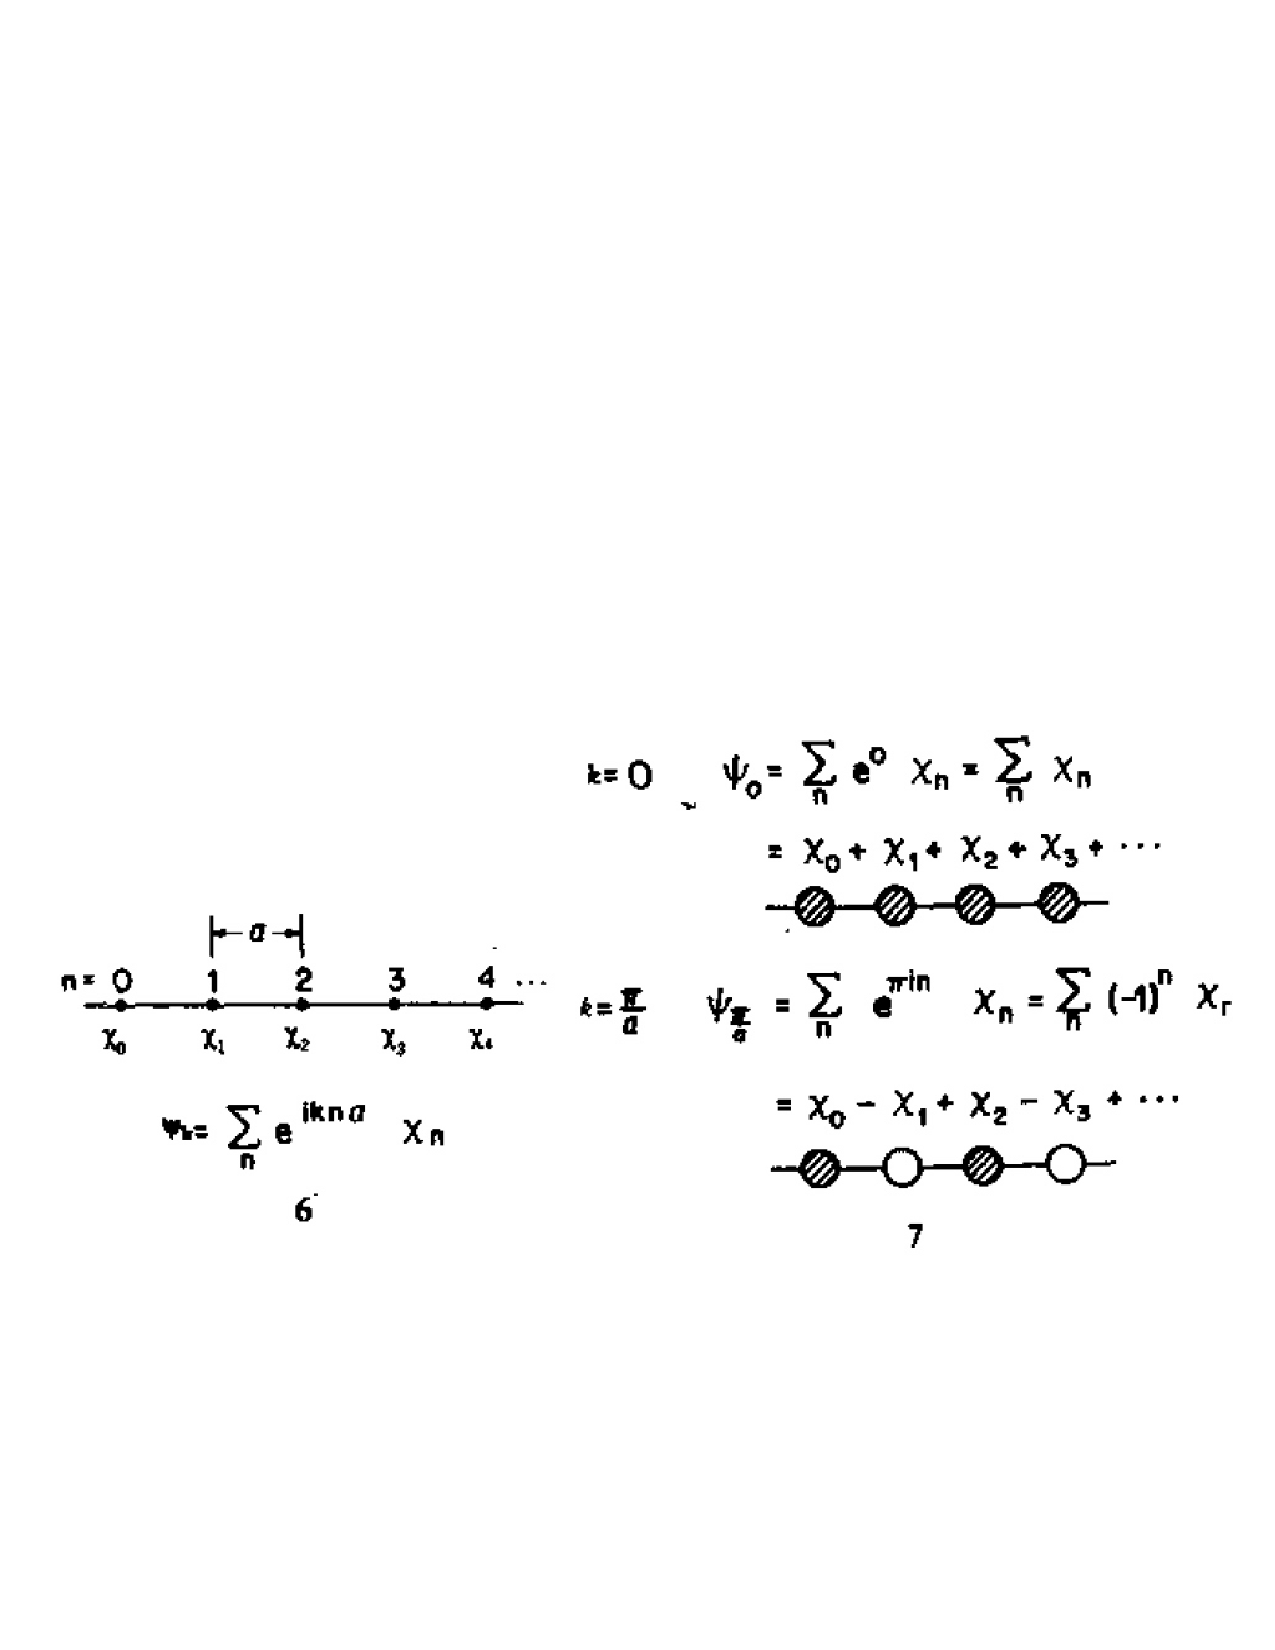
\includegraphics[height=0.5in,width=1.4in,viewport=25 218 595 440,clip]{Figures/Hydrogen-Psi.pdf}}\\
\subfigure[分子轨道与能带]{
\label{fig:Hydrogen-Band-1D}
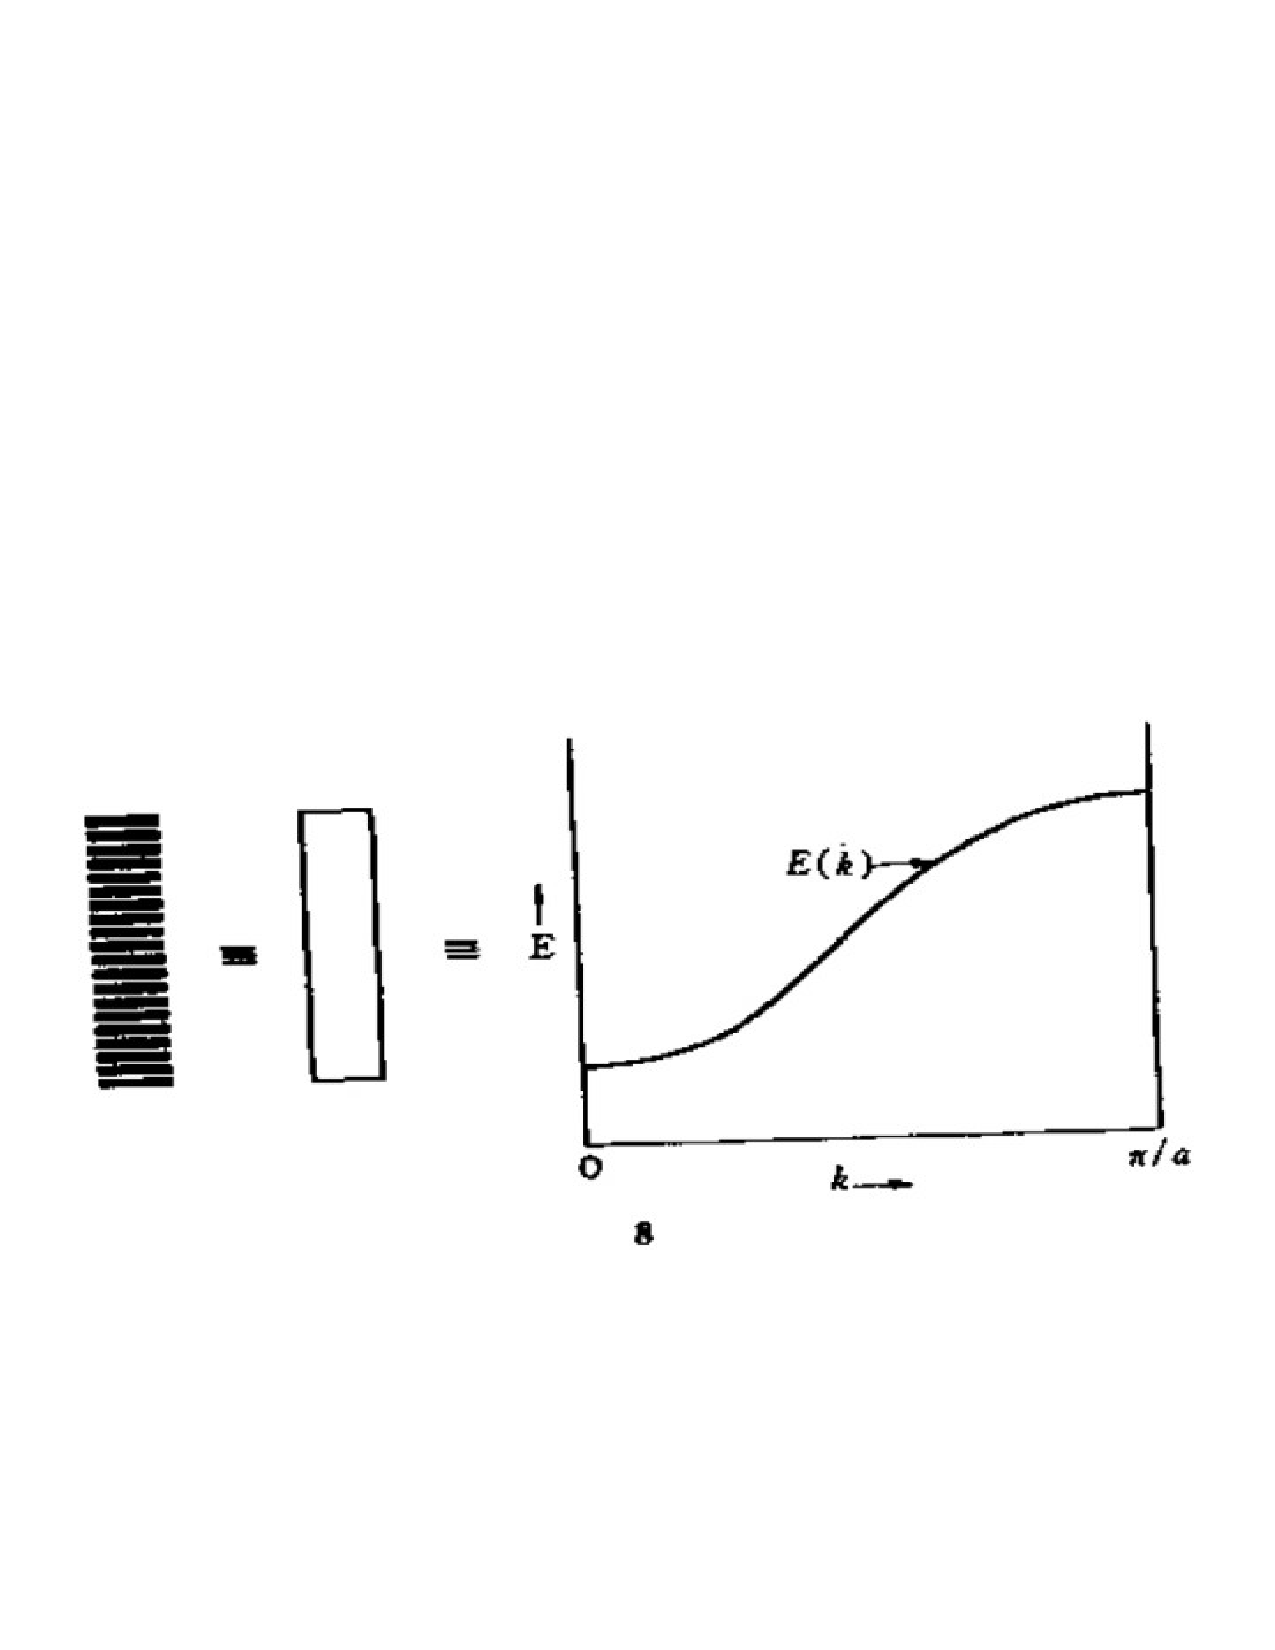
\includegraphics[height=0.6in,width=1.4in,viewport=35 215 575 450,clip]{Figures/Hydrogen-Band-1D.pdf}}
\subfigure[$d$\,轨道]{
\label{fig:Hydrogen-d-Band-1D}
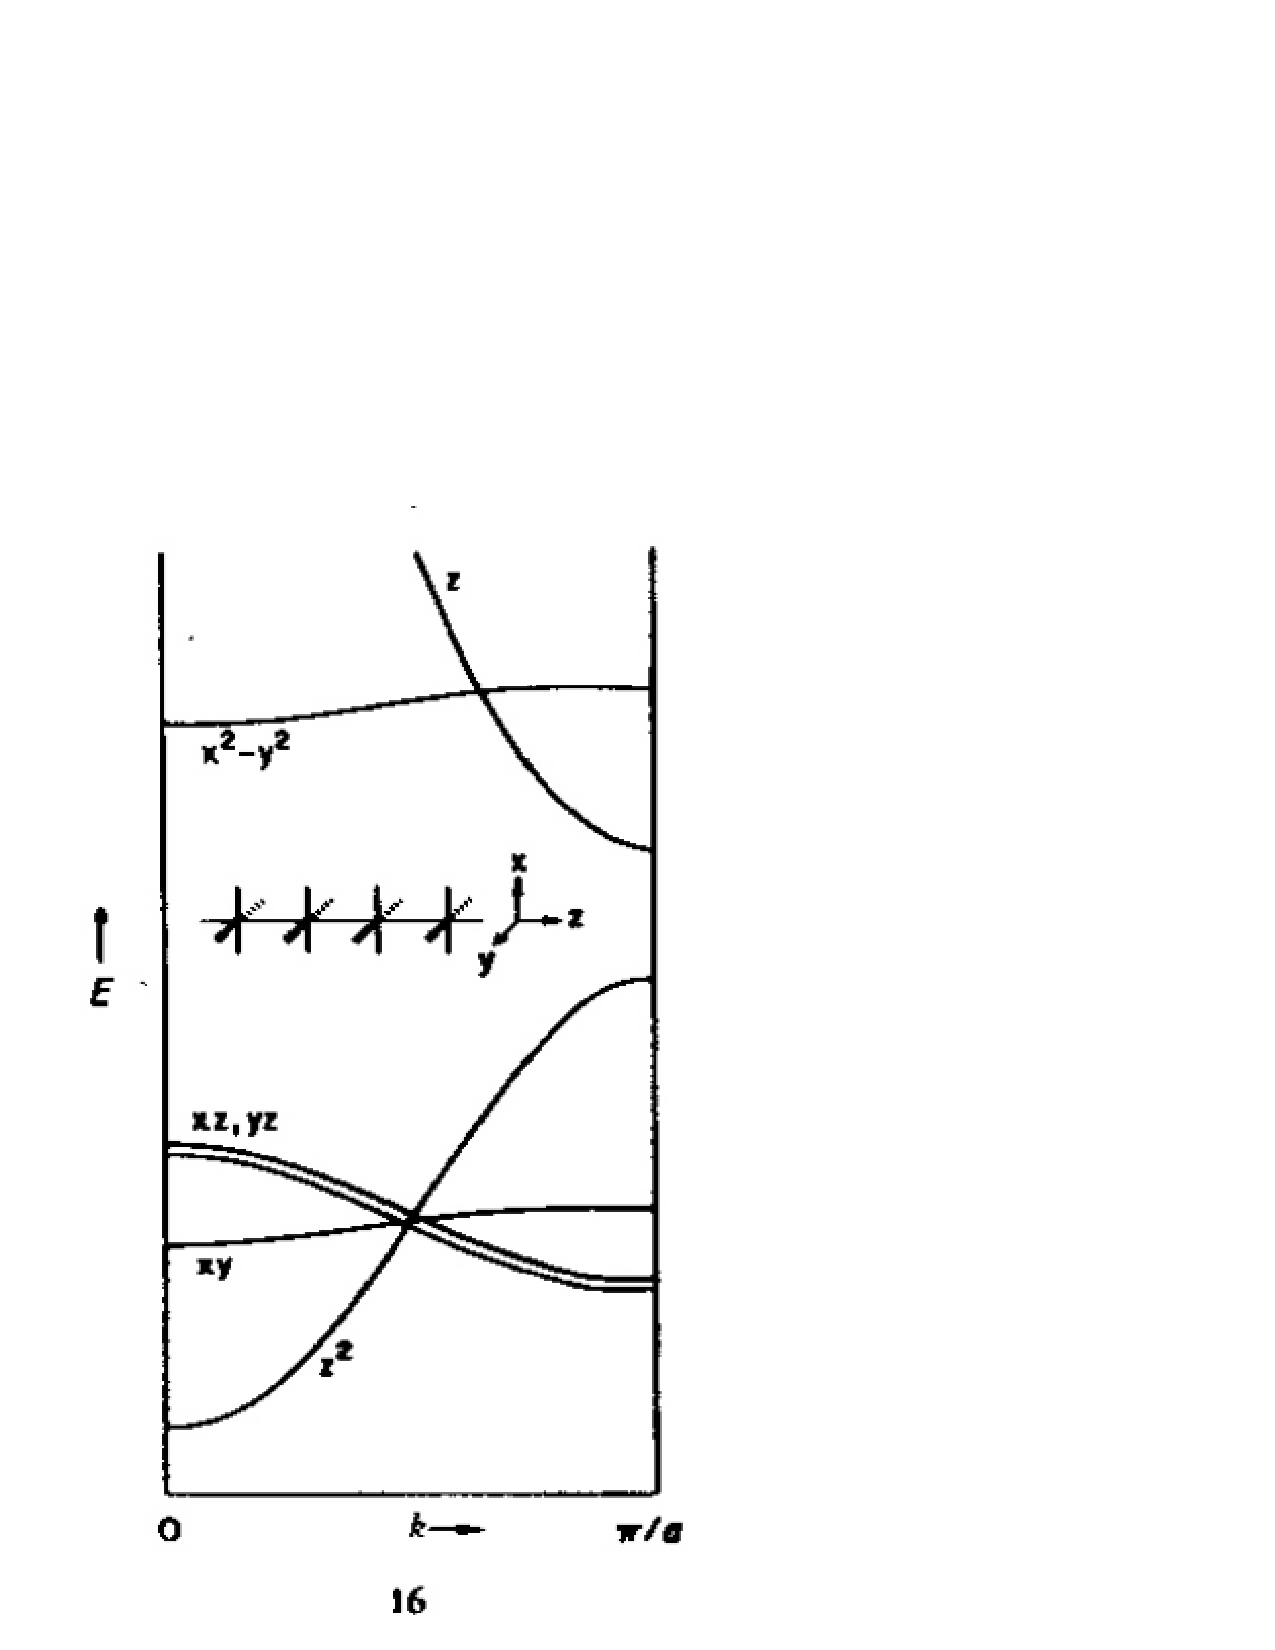
\includegraphics[height=1.0in,width=0.7in,viewport=40 45 330 535,clip]{Figures/Hydrogen-d-Band-1D.pdf}}
\caption{\small \textrm{The Band-structure from Molecular-orbital.}}%
\label{Band-Structure-1}
\end{figure} 
}

\frame
{
\frametitle{能带、$\vec k$空间与\textrm{Fermi}面}
\vspace{30pt}
\begin{figure}[h!]
\centering
\hspace*{-0.30in}
\subfigure[\textrm{Band structure}]{
\label{Band_Gap_Fermi-1}
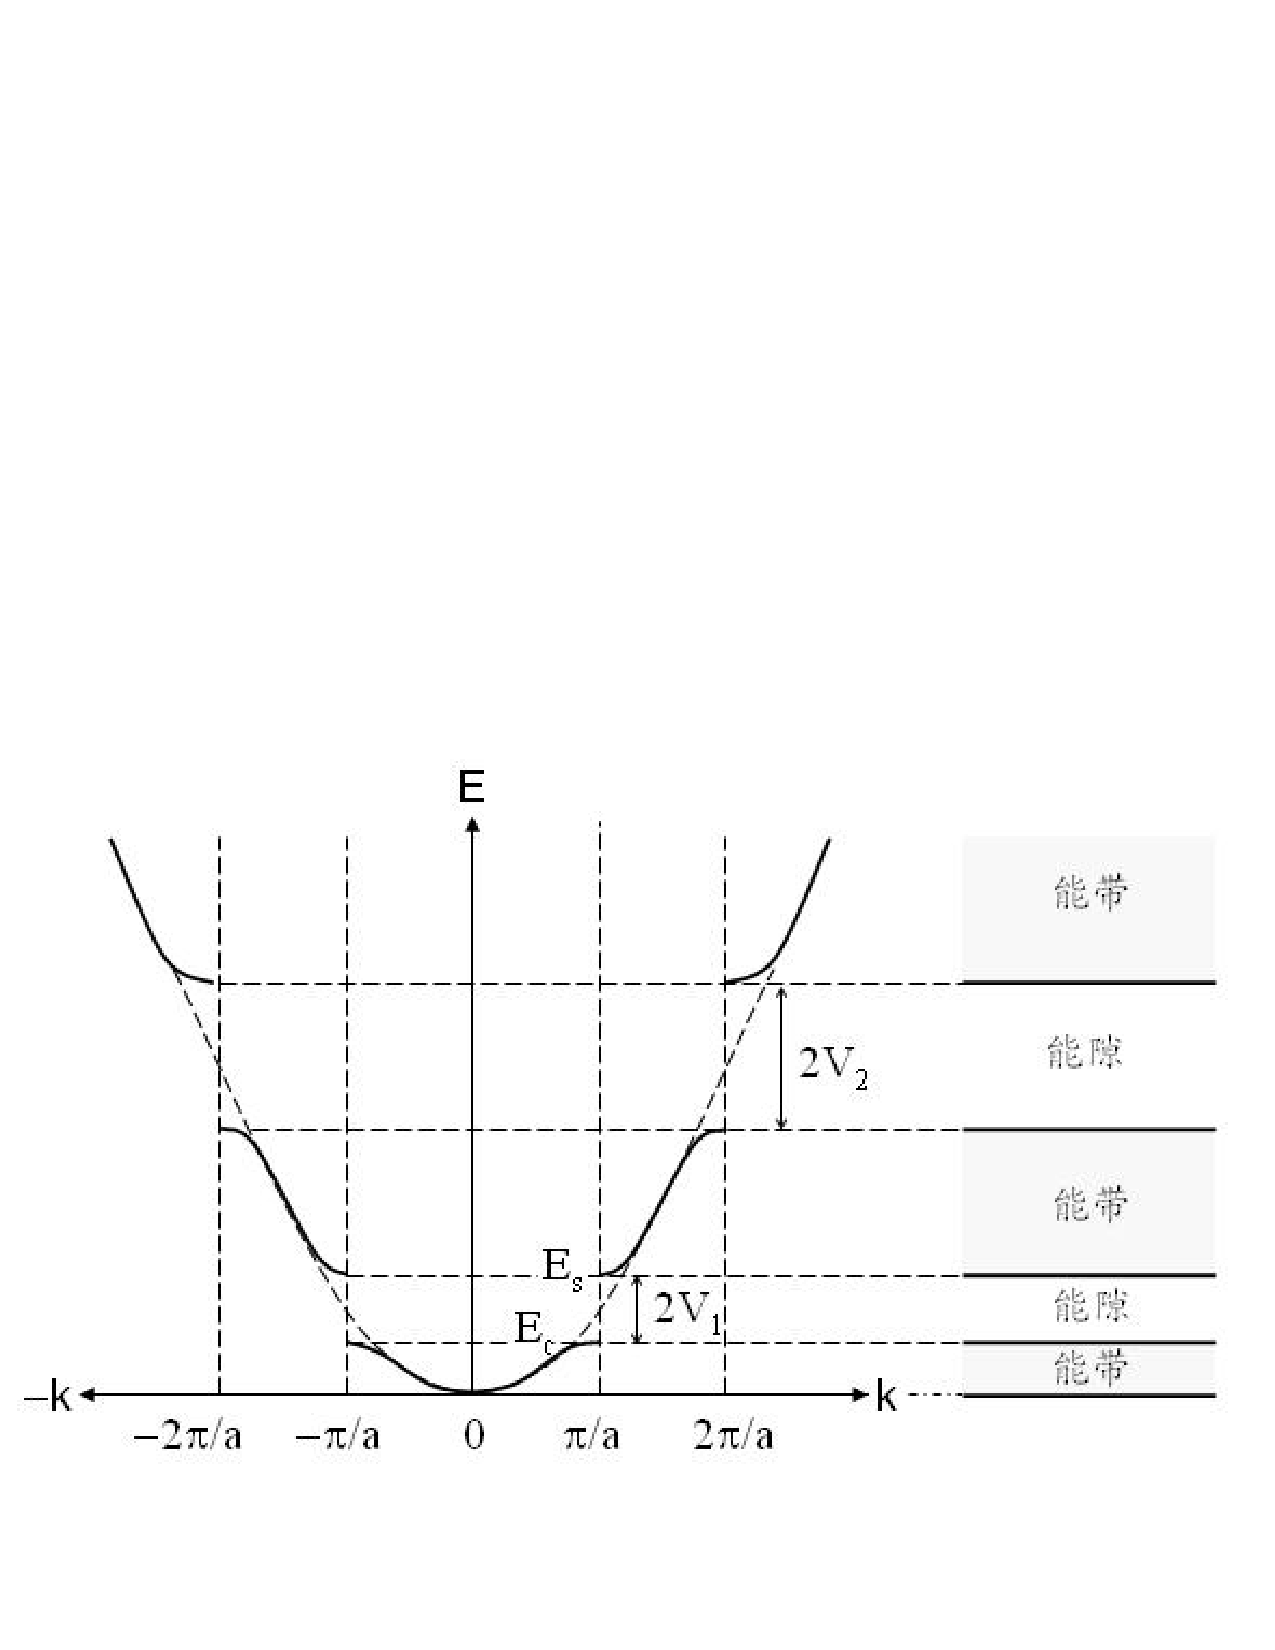
\includegraphics[height=1.3in,width=2.3in,viewport=10 90 570 380,clip]{Figures/Band_Gap.pdf}}
\subfigure[\textrm{Brillouin Zone}]{
\label{Band_Gap_Fermi-2}
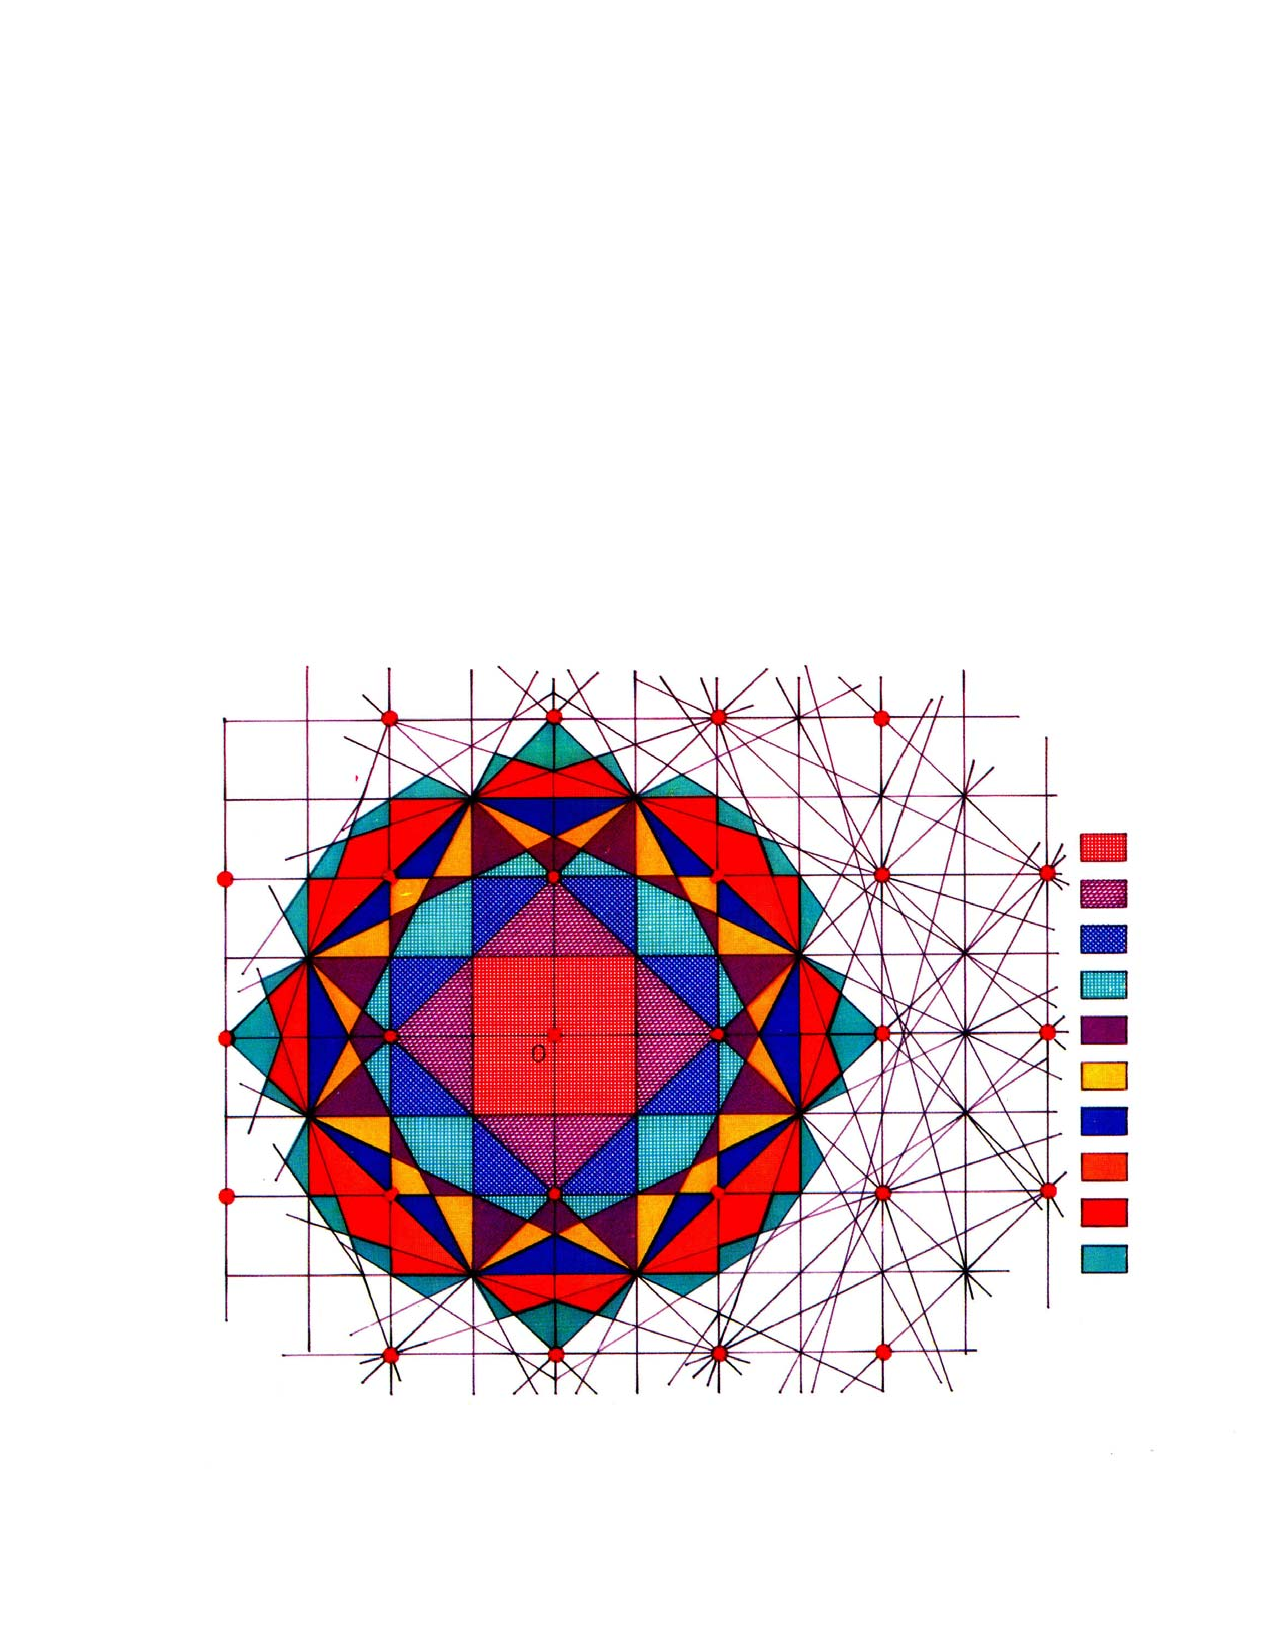
\includegraphics[height=1.28in,width=1.75in,viewport=100 120 545 470,clip]{Figures/2D_Brillouin-Zone.pdf}}
\label{Band_Gap_Fermi}
\end{figure}
}

\frame
{
	\frametitle{体心立方体系的\textrm{Brillouin}区与能带}
\vspace{10pt}
\begin{figure}[h!]
\centering
\hspace*{-0.30in}
\subfigure[\textrm{Brillouin Zone of BCC lattice}]{
\label{Brillouin_Zone_BCC}
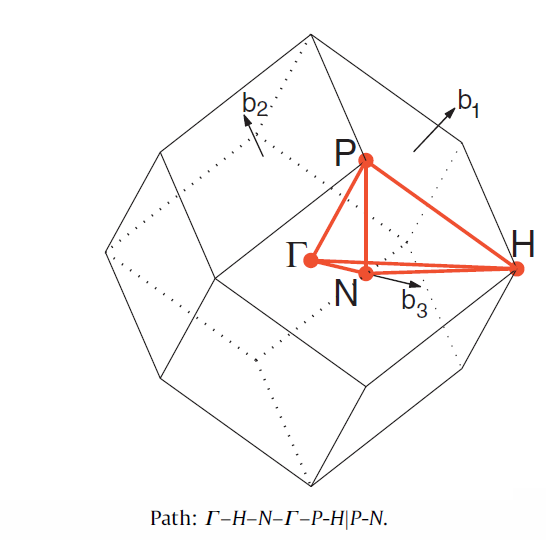
\includegraphics[height=2.1in,width=1.9in,viewport=80 0 550 520,clip]{Figures/Brillouin-Zone_BCC.png}}
\subfigure[\textrm{Band structure of GeF$_4$}]{
\label{Band_Gap_GeF4}
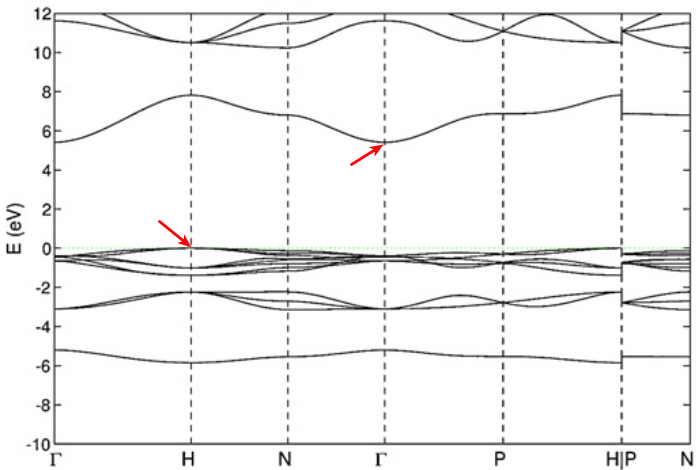
\includegraphics[height=2.10in,width=1.95in,viewport=0 0 700 500,clip]{Figures/Band-Struct_GeF4.png}}
\label{Band_Gap_BCC_GeF4}
\end{figure}
}

\subsection{周期体系基态总能量}
\frame
{
	\frametitle{晶体总能量的一般表示}
周期体系的总能量$E_T$可表示为晶格中的电子能量$E_{e-e}$与离子实排斥能$E_{N-N}$之和:~
	\begin{displaymath}
		E_T=E_{e-e}+E_{N-N}=T[\rho]+E_{ext}+E_{\mathrm{Coul}}+E_{\mathrm{XC}}+E_{N-N}
	\end{displaymath}
根据\textrm{Kohn-Sham}方程,其中动能泛函用单电子能量表示为
\begin{displaymath}
	T[{\rho}]=\sum_in_i\langle\psi_i|\varepsilon_i-V_{\mathrm{KS}}|\psi_i\rangle
\end{displaymath}
$n_i$是$\psi_i$上的电子占据数,$\varepsilon_i$是其能量本征值,因此有
\begin{displaymath}
	\hspace*{-12.0pt}	E_T=\sum_in_i\varepsilon_i-\dfrac12\int\int\mathrm{d}\vec r\mathrm{d}\vec r\dfrac{\rho(\vec r)\rho(\vec r^{\prime})}{|\vec r-\vec r^{\prime}|}+\int\mathrm{d}\vec r\rho(\vec r)[\epsilon_{\mathrm{XC}}(\vec r)-V_{\mathrm{XC}}(\vec r)]+E_{N-N}
\end{displaymath}
}

\frame
{
	\frametitle{晶体总能量倒空间的表示}
周期体系的总能量表达式在动量空间($\vec K$空间)计算更方便
\begin{displaymath}
	\hspace*{-15.0pt}	E_T=\textcolor{red}{\sum_in_i\varepsilon_i}-\dfrac{\Omega}2\sum_{\textcolor{red}{\vec k\neq 0}}\rho^{\ast}(\vec k)V_{\mathrm{Coul}}(\vec k)+\Omega\sum_{\vec k}\rho^{\ast}(\vec k)[\epsilon_{\mathrm{XC}}(\vec k)-V_{\mathrm{XC}}(\vec k)]+E_{N-N}
\end{displaymath}
其中$V_{\mathrm{Coul}}(\vec k)$、$\epsilon_{\mathrm{XC}}(\vec k)$与$\rho^{\ast}(\vec k)$分别是\textrm{Coulomb}相互作用、单个电子的交换-相关能、交换-相关势和电子密度的\textrm{Fourier}分量。

由\textrm{Poisson}方程
\begin{displaymath}
	\nabla^2V_{\mathrm{Coul}}(\vec r)=-4\pi\rho(\vec r)
\end{displaymath}
的\textrm{Fourier}展开有
\begin{displaymath}
	V_{\mathrm{Coul}}(\vec k)=\dfrac{4\pi\rho^{\ast}(\vec k)}{|\vec k|^2}
\end{displaymath}
交换-相关势和交换-相关能的计算一般先在实空间计算$\epsilon_{\mathrm{XC}}(\vec r)$和$V_{\mathrm{XC}}(\vec r)$后,再通过\textrm{Fourier}变换到动量空间,得到$\epsilon_{\mathrm{XC}}(\vec k)$和$V_{\mathrm{XC}}(\vec k)$
}

\frame
{
	\frametitle{晶体相互作用的计算}
	离子间\textrm{Coulomb}相互作用能之和
	{\fontsize{6.5pt}{4.2pt}\selectfont{
	\begin{displaymath}
		E_{N-N}=\dfrac12\sum_{\vec R,s}\sideset{}{^{\prime}}\sum_{\vec R^{\prime},\vec s^{\prime}}\dfrac{Z_sZ_{s^{\prime}}}{|\vec R+\vec r_s-\vec R^{\prime}-\vec r_s^{\prime}|}
	\end{displaymath}
这里$Z_s$是离子实的电荷数,$\vec R$表示晶格点的位矢,$\vec r_s$代表元胞内原子的相对位矢。}}
	
	能量本征值求和中包含$V_{ext}$的贡献:~在不存在其他外场时,$V_{ext}$只考虑离子-电子的\textrm{Coulomb}相互作用:
	{\fontsize{6.5pt}{4.2pt}\selectfont{
	\begin{displaymath}
		\begin{aligned}
			V_{ext}(\vec r)&=\sum_{\vec R,s}\dfrac{-Z_s}{|\vec r-\vec R-\vec r_s|}\\
			&\equiv\sum_{\vec R,s}v_{ext}^s(\vec r-\vec R-\vec r_s)
		\end{aligned}
	\end{displaymath}}}
\textcolor{red}{\textbf{注意}}:~总能量在动量空间求和时,
\begin{itemize}
	\item 离子相互作用$E_{N-N}$求和包含无穷多项,是发散的
	\item 电子相互作用$V_{\mathrm{Coul}}(\vec k=0)$是发散的
	\item 离子-电子相互作用$V_{\mathrm{ext}}(\vec k=0)$是发散的
\end{itemize}
}

\frame
{
	\frametitle{晶体总能量计算的奇点排除}
为了克服总能量求和的发散问题,考虑到体系呈电中性,发散项之和应为常数,因此求解\textrm{Kohn-Sham}方程时,先将$V_{\mathrm{Coul}}(\vec k=0)$和$V_{ext}(\vec k=0)$同时置为零,这相当于\textcolor{red}{将势能作一平移,或者说重新定义势能零点,而在总能量计算中补偿这一平移。}

{\fontsize{6.5pt}{4.2pt}\selectfont{
	发散项之和为:
	\begin{displaymath}
		\begin{aligned}
			\lim_{\vec k\rightarrow0}\Omega&\bigg[\dfrac12V_{\mathrm{Coul}}(\vec k)+\sum_sv_{ext}^s(\vec k)\bigg]\rho^{\ast}(\vec k)+\dfrac12\sum_{\vec R,s}\sideset{}{^{\prime}}\sum_{\vec R^{\prime},\vec s^{\prime}}\dfrac{Z_sZ_{s^{\prime}}}{|\vec R+\vec r_s-\vec R^{\prime}-\vec r_s^{\prime}|}\\
			=&\sum_s\alpha_s\sum_sZ_s+\textcolor{magenta}{E_{\mathrm{Ewald}}}
		\end{aligned}
	\end{displaymath}}}
由此得到的总能量表达式是
\begin{displaymath}
	\begin{aligned}
		E_T=&\sum_i\varepsilon_i-\dfrac{\Omega}2\sum_{\vec k\neq0}\rho^{\ast}(\vec k)V_{\mathrm{Coul}}(\vec k)\\
		&+\Omega\sum_{\vec k}\rho^{\ast}(\vec k)[\epsilon_{\mathrm{XC}}(\vec k)-V_{\mathrm{XC}}(\vec k)]\\
		&+\sum_s\alpha_s\sum_sZ_s+E_{\mathrm{Ewald}}
	\end{aligned}
\end{displaymath}
}

\frame
{
	\frametitle{离子间相互作用的\textrm{Ewald}求和}
	\begin{displaymath}
		\begin{aligned}
			E_{\textrm{Ewald}}=&\dfrac12\sum_{\vec R,s}\sideset{}{^{\prime}}\sum_{\vec R^{\prime},\vec s^{\prime}}\dfrac{Z_sZ_{s^{\prime}}}{|\vec R+\vec r_s-\vec R^{\prime}-\vec r_{s^{\prime}}|}-\lim_{\vec k\rightarrow0}\dfrac12\times\dfrac{4\pi(\sum_sZ_s)^2}{\Omega|\vec k|^2}\\
			=&\dfrac12\sum_{\vec R,s}\sideset{}{^{\prime}}\sum_{\vec R^{\prime},\vec s^{\prime}}\dfrac{Z_sZ_{s^{\prime}}}{|\vec R+\vec r_s-\vec R^{\prime}-\vec r_{s^{\prime}}|}-\dfrac1{2\Omega}\sum_{s,s^{\prime}}\int\mathrm{d}\vec r\dfrac{Z_sZ_{s^{\prime}}}r\\
			=&\sum_{s,s^{\prime}}Z_sZ_{s^{\prime}}\bigg\{\dfrac{2\pi}{\Omega}\sum_{\vec k\neq 0}\cos[\vec k\cdot(\vec r_s-\vec r_{s^{\prime}})]\dfrac{\mathrm{e}^{-|\vec k|^2/4\eta^2}}{|\vec k|^2}\\
			&-\dfrac{\pi}{2\eta^2\Omega}+\dfrac12\sum_{\vec R}\dfrac{\mathrm{erf}(\eta x)}x\bigg|_{\vec R+\vec r_s-\vec r_s^{\prime}\neq0}-\dfrac{\eta}{\sqrt{\pi}}\delta_{s,s^{\prime}}\bigg\}
		\end{aligned}
	\end{displaymath}
	$\mathrm{erf}(x)$是误差函数,$\eta$原则上是任意参数。$\alpha_s$由$v_{ext}^s(\vec r)$确定:
	\begin{displaymath}
		\alpha_s=\lim_{\vec k\rightarrow0}\bigg[v_{ext}^s(\vec k)+\dfrac{4\pi Z_s}{\Omega|\vec k|^2}\bigg]=\dfrac1{\Omega}\int\mathrm{d}\vec r\bigg[v_{ext}^s(\vec r)+\dfrac{Z_s}r\bigg]
	\end{displaymath}
}

\frame
{
	\frametitle{总能量表达式}
\begin{figure}[h!]
\centering
\vspace*{-0.18in}
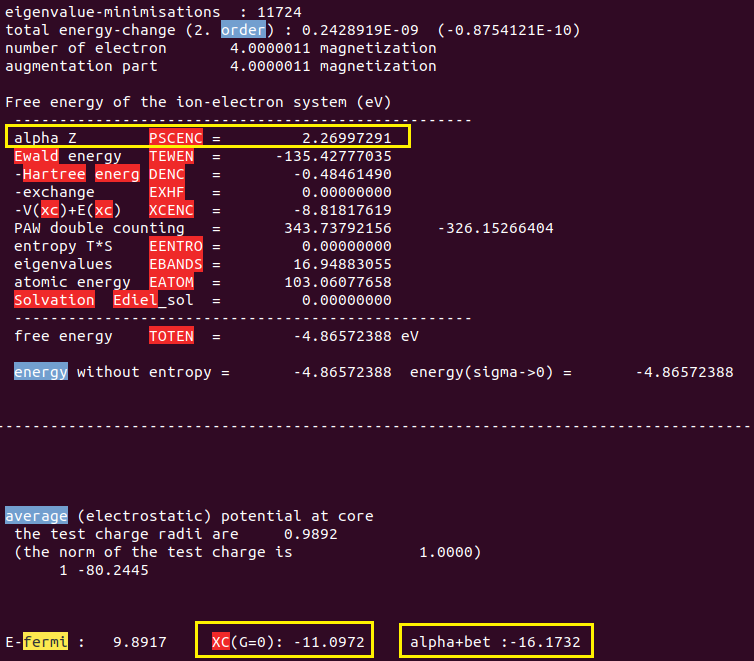
\includegraphics[height=1.95in,width=2.3in,viewport=0 0 600 495,clip]{Figures/VASP_Total_ENE.png}
\caption{\small \textrm{The Total-E calculated by VASP.}}%(与文献\cite{EPJB33-47_2003}图1对比)
\label{TOTEN_VASP}
\end{figure}
}

\frame
{
	\frametitle{\textrm{DFT-SCF}}
\begin{figure}[h!]
\centering
\vspace*{-0.25in}
\hspace*{-0.80in}
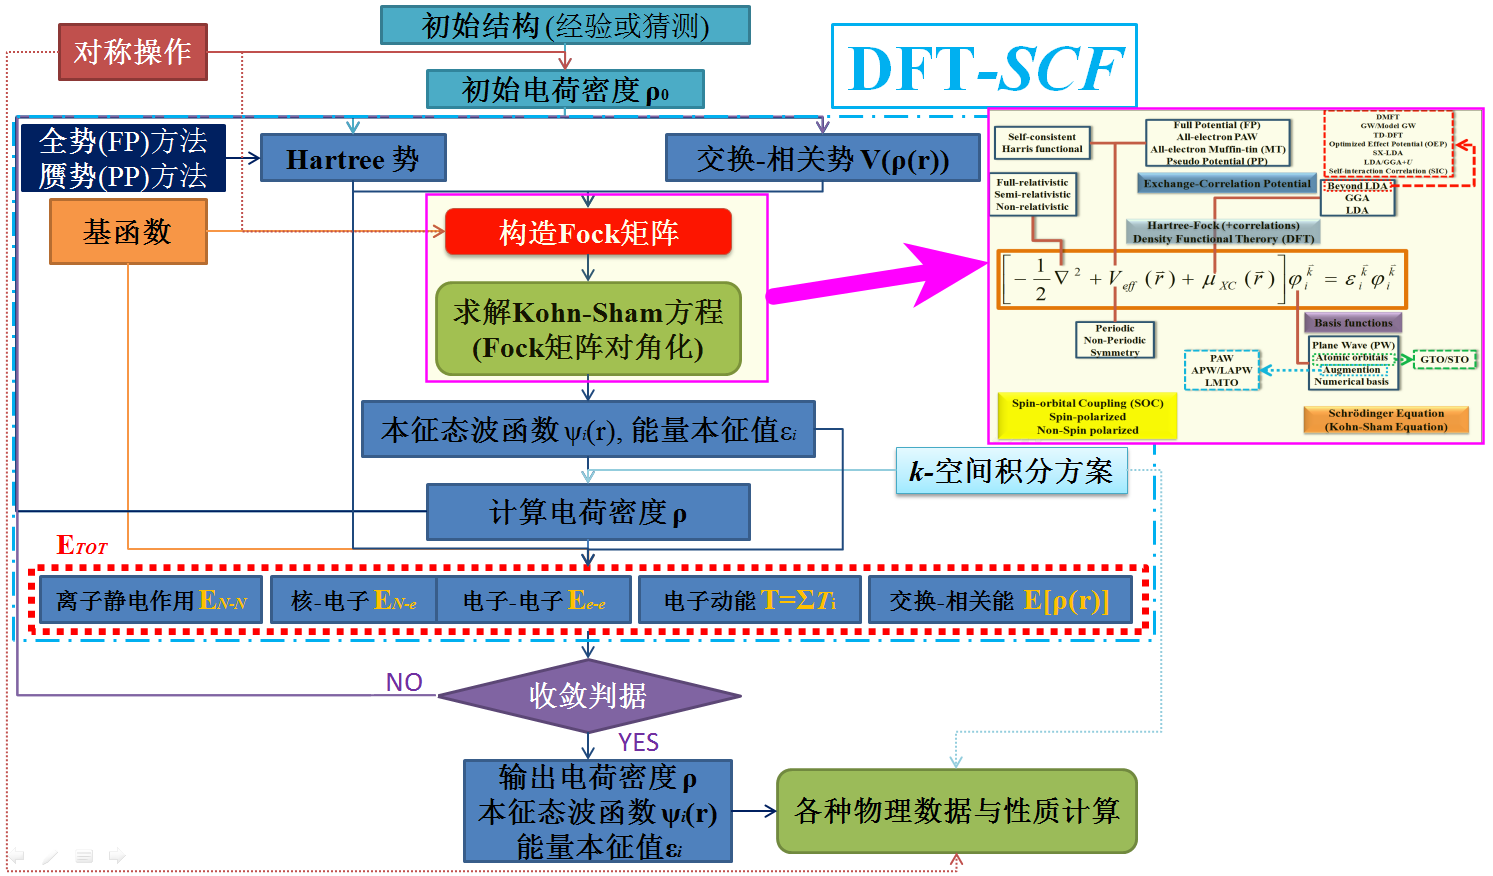
\includegraphics[height=2.80in,width=4.95in,viewport=5 3 1490 870,clip]{Figures/DFT-SCF_2.png}
%\caption{\small \textrm{Pseudopotential for metallic sodium, based on the empty core model and screened by the Thomas-Fermi dielectric function.}}%(与文献\cite{EPJB33-47_2003}图1对比)
\label{Pseudo-NC}
\end{figure}
}

\section{材料电子结构计算方法}       %Bookmark
\frame
{
\frametitle{周期体系的波函数}
物质的电子体系,可分为芯层分子和价层电子。芯电子能量低,受周围化学环境影响很小,基本保持原子属性;价层电子相互作用较强,对化学环境较为敏感。一般地,价电子波函数在原子间区域(\textrm{Interstitial}区)的变化平缓,在临近原子核附近区域(\textrm{Muffin-tin}球内),会出现剧烈振荡(与芯层波函数正交)。
\begin{figure}[h!]
\centering
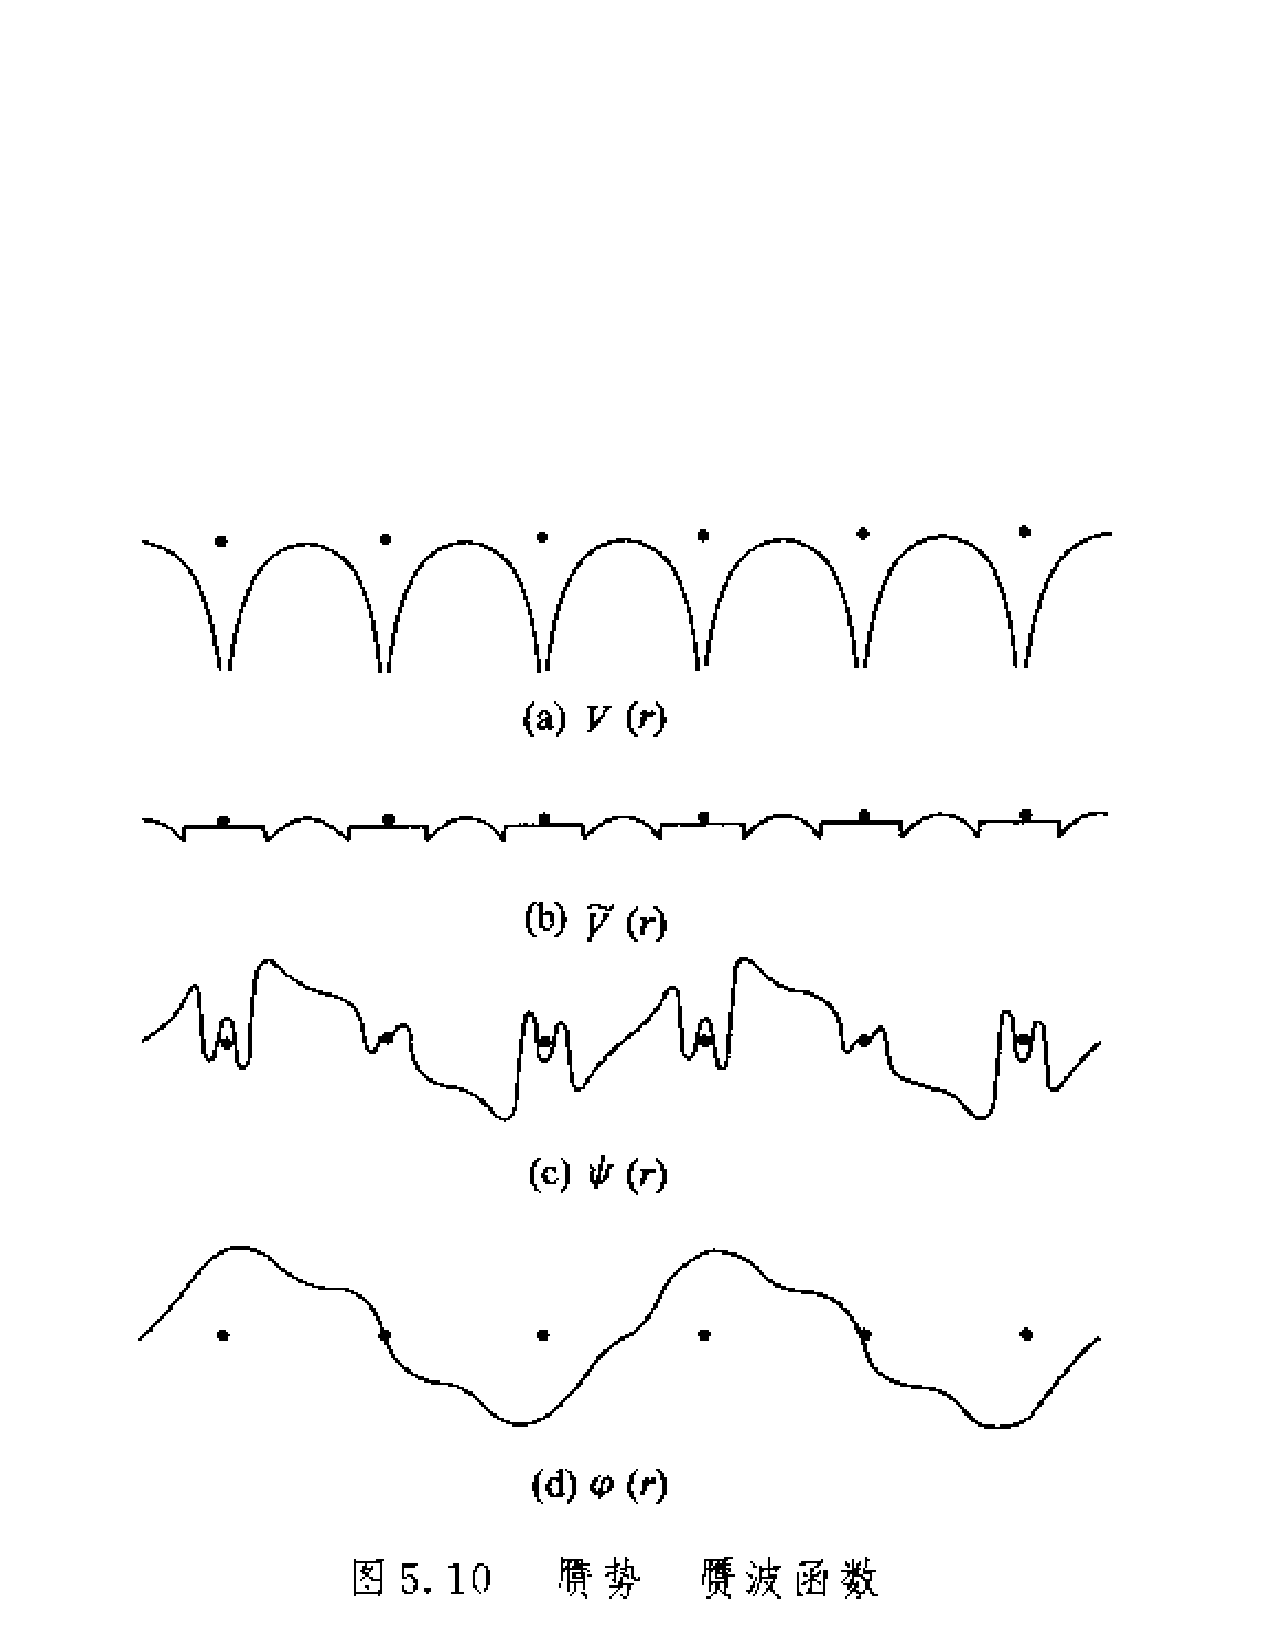
\includegraphics[height=0.8in,width=4.in,viewport=41 433 539 546,clip]{Figures/Pseudo_wave.pdf}\\
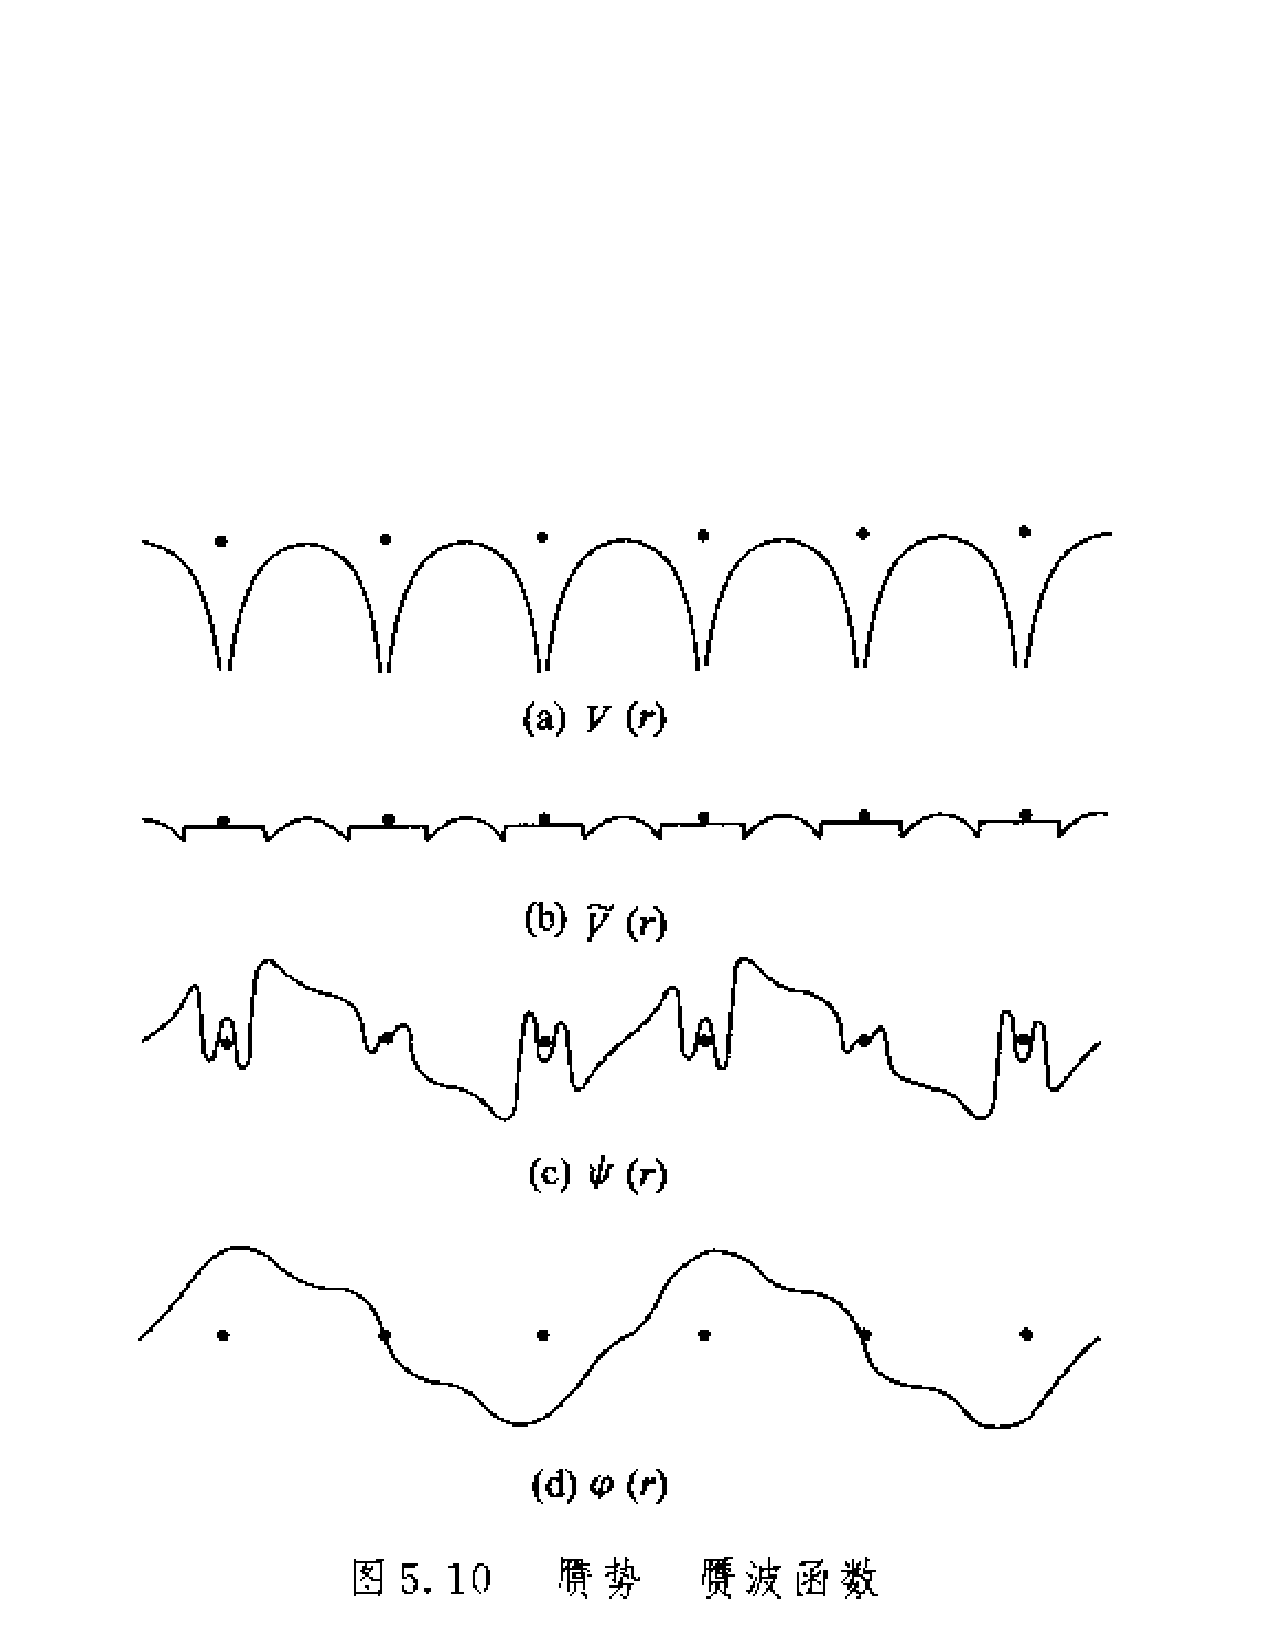
\includegraphics[height=0.8in,width=4.in,viewport=41 210 539 339,clip]{Figures/Pseudo_wave.pdf}
\caption{\small \textrm{The periodic Potential and the wave functions in crystal.}}%(与文献\cite{EPJB33-47_2003}图1对比)
\label{Potential-Wave}
\end{figure}
}

\frame
{
%\frametitle{The methods on band structure calculation}
\frametitle{能带计算方法}
%\vskip 10pt
%\textrm{The mainly difference of all these methods below: the basis sets and the construction of the potential}
\vskip 10pt
常用的计算方法
\begin{itemize}%[+-| alert@+>]
%\begin{enumerate}%[+-| alert@+>]
\setlength{\itemsep}{12pt}
%  \item \textrm{Plane wave and the pseudo-potential}
	\item	平面波方法
	\item	正交平面波\textrm{(The orthogonalized plane wave, OPW)}和赝势\textrm{(Pseudo-potential, PP)}方法\upcite{Singh_Book,PRB41-7892_1990,JPCM6-8245_1994}
	\item	缀加平面波\textrm{(Augmented plane wave, APW)}方法
	\item	\textrm{MT}轨道\textrm{(Muffin-tin orbitals, MTO)}方法
	\item	投影子缀加波\textrm{(Projector Augmented Wave, PAW)}方法\upcite{PRB50-17953_1994,PRB59-1758_1999}
\end{itemize}
\vskip 5pt 各种方法的\textcolor{red}{主要区别}:~\textcolor{blue}{势函数的处理}与\textcolor{blue}{所选基函数类型}不同
}

\frame
{
	\frametitle{能带计算方法}
\begin{figure}[h!]
\centering
\vspace*{-0.25in}
%\hspace*{-0.80in}
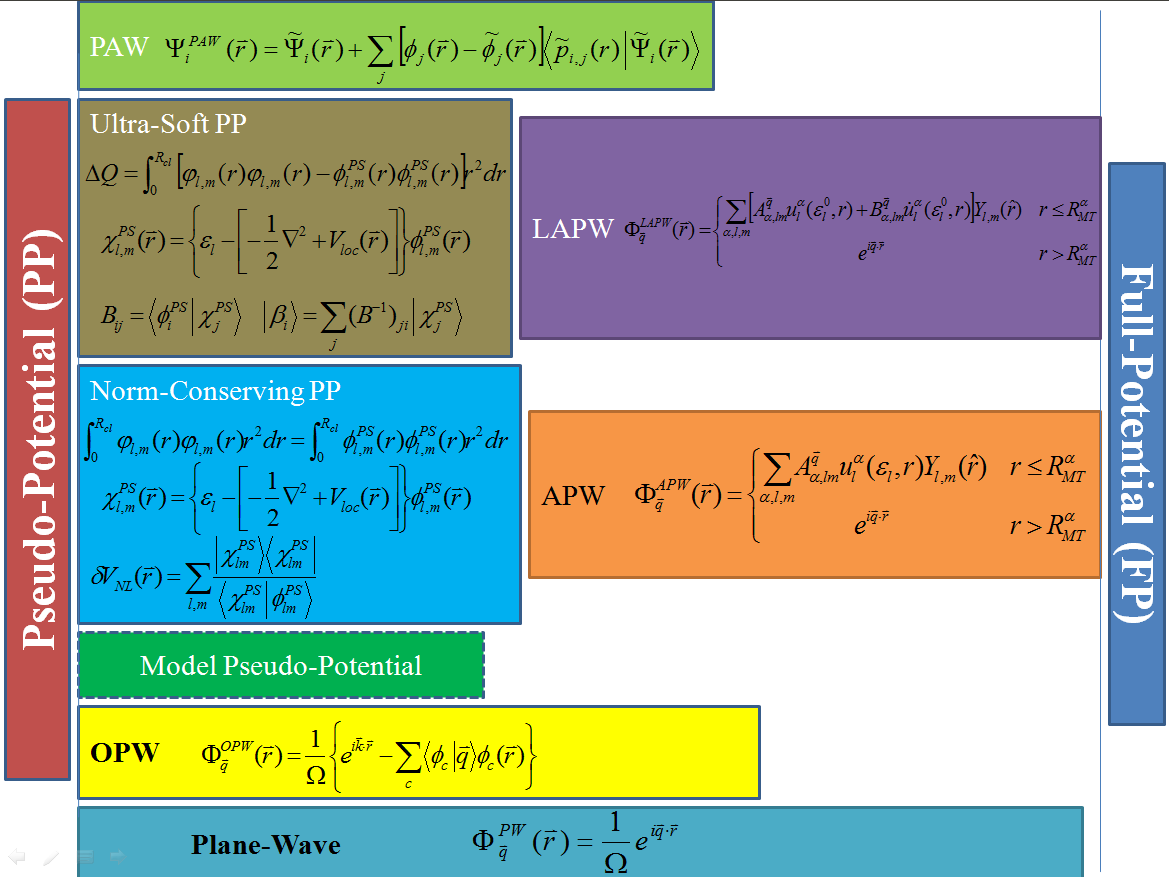
\includegraphics[height=2.80in,width=4.10in,viewport=0 0 1190 876,clip]{Figures/Pseudo-Full_Potential.png}
%\caption{\small \textrm{Pseudopotential for metallic sodium, based on the empty core model and screened by the Thomas-Fermi dielectric function.}}%(与文献\cite{EPJB33-47_2003}图1对比)
\label{Pseudo-Full_Poential}
\end{figure}
}

%\section{Induction on DFT and solid-state physics}       %Bookmark
\frame
{
	\frametitle{球形势对平面波的散射与相移}
\begin{figure}[h!]
\centering
\vspace*{-0.26in}
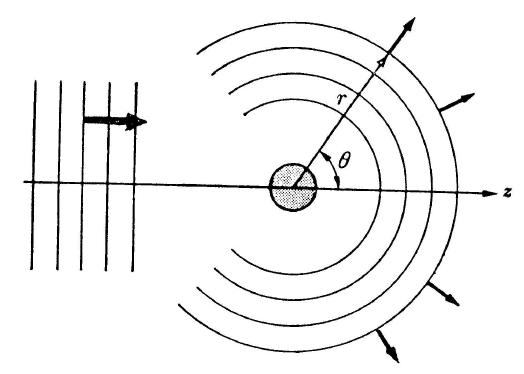
\includegraphics[height=0.90in,width=1.24in,viewport=0 0 400 300,clip]{Figures/Pseudo-scatter.jpg}
\caption{\small \textrm{Schematic illustration of scattering of a plane wave by a spherical potential.}}%(与文献\cite{EPJB33-47_2003}图1对比)
\label{Pseudo-scatter}
\end{figure}
$$\mathrm{e}^{\mathrm{i}\vec q\cdot\vec r}=4\pi\sum_{lm}\mathrm{i}^lj_l(\vec q\cdot\vec r)Y_{lm}^{\ast}(\hat{\vec q})Y_{lm}(\hat{\vec r})=\sum_{l}(2l+1)\mathrm{i}^lj_l(qr)P_{l}(\cos\theta)$$
%$$\mathrm{e}^{\mathrm{i}\vec q\cdot\vec r}=\mathrm{e}^{\mathrm{i}qr\cos(\theta)}=\sum_{l}(2l+1)\mathrm{i}^lj_l(qr)P_{l}[\cos(\theta)]$$
$$\Psi_l^{>}(\varepsilon,r)=C_l\bigg[j_l(\kappa r)-\tan\eta_l(\varepsilon)n_l(\kappa r)\bigg]\quad\text{其中}\kappa^2=\varepsilon$$
$$D_l(\varepsilon,r)\equiv r\psi_l^{\prime}(r)/\psi_l(r)=r\dfrac{\mathrm{d}}{\mathrm{d}r}\ln\psi_l(r)$$
$$\tan\eta_l(\varepsilon)=\dfrac{R\frac{\mathrm{d}}{\mathrm{d}r}j_l(\kappa r)|_R-D_l(\varepsilon)j_l(\kappa R)}{R\frac{\mathrm{d}}{\mathrm{d}r}n_l(\kappa r)|_R-D_l(\varepsilon)n_l(\kappa R)}$$
%$$t(\theta)=\dfrac{4\pi}{\sqrt\varepsilon}\sum_l(2l+1)\bigg[\mathrm{e}^{2\mathrm{i}\eta_l}-1\bigg]P_l(\cos\theta)$$
%$$\eta_l(\varepsilon)=p_l\pi+\delta_l(\varepsilon)$$
}

\frame
{
\frametitle{赝势方法}
%赝势(\textrm{Pseudo Potential, PP})方法是在正交平面波的基础上发展起来的,构造出平缓的势函数代替核的强吸引作用和芯层电子的排斥作用,用平缓的函数取代波函数近核时的震荡。
\begin{itemize}
\setlength{\itemsep}{5pt}
	\item 赝势-平面波方法,只需要少量平面波可展开赝波函数,大大提升了计算效率;但是赝波函数不能很好地反映与电子近核行为有关的性质。
	\item 赝势的构造并不唯一,考核构造赝势的两大指标:~\\“柔软程度”\textrm{(Soft)}与“可移植性”\textrm{(transferability)}
\end{itemize}
\begin{figure}[h!]
\centering
\vspace*{-0.10in}
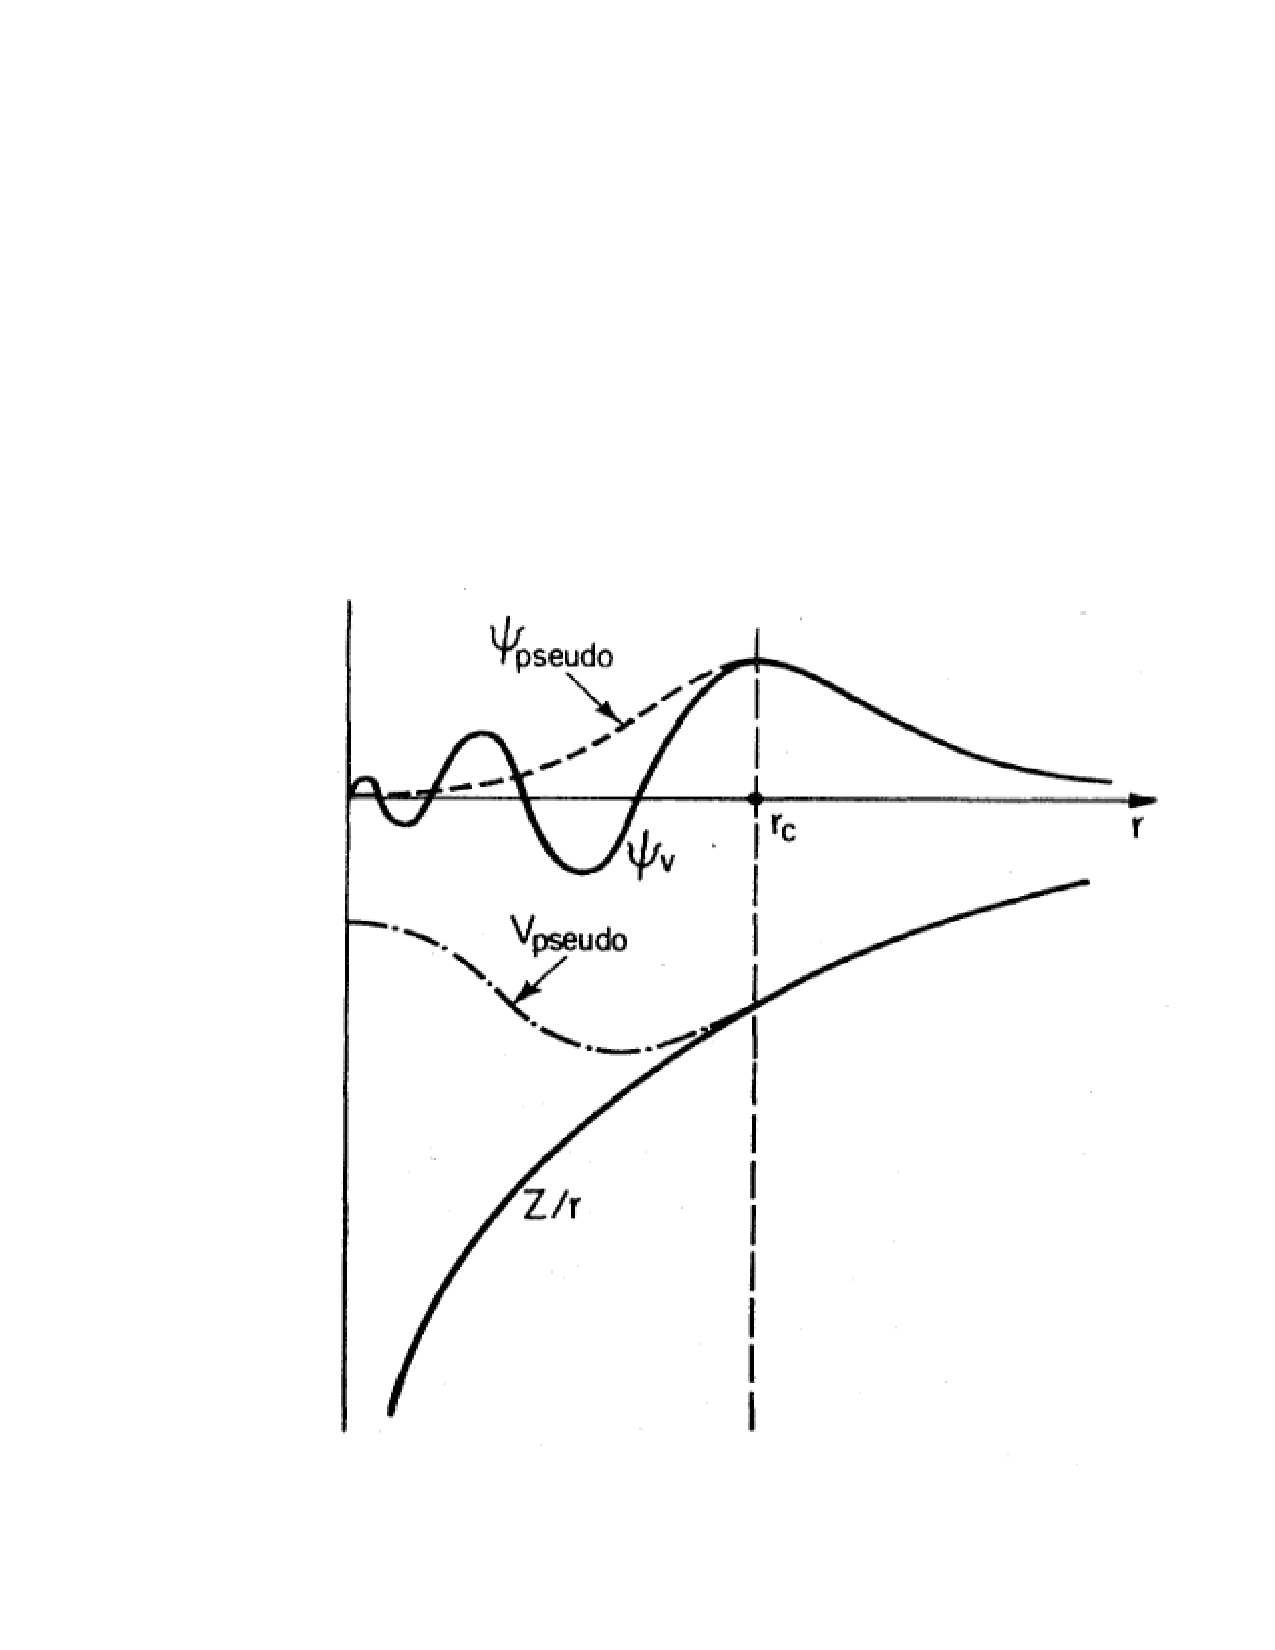
\includegraphics[height=1.35in,width=1.42in,viewport=154 100 562 508,clip]{Figures/Pseudo.pdf}
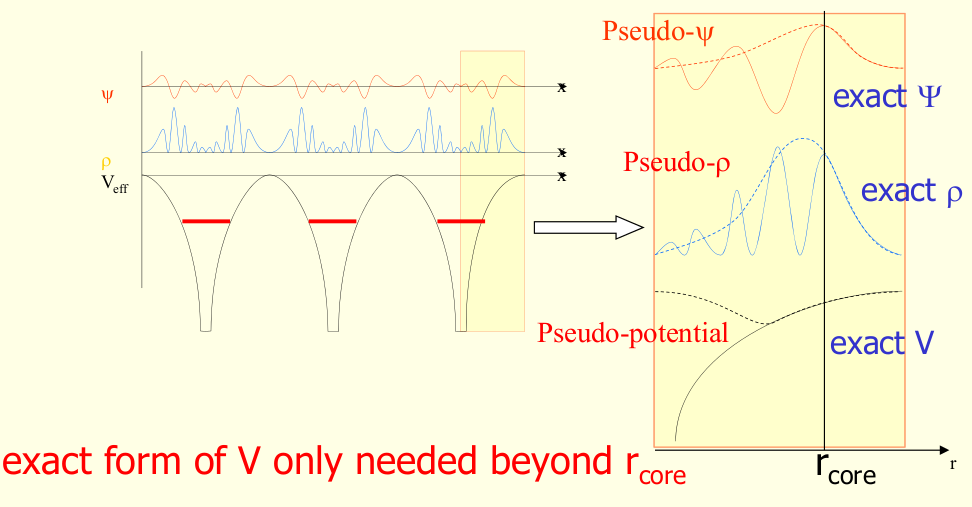
\includegraphics[height=1.35in,width=2.57in,viewport=1 1 980 500,clip]{Figures/Pseudo-2.png}
\caption{\small \textrm{The Pseudo wave function and Pseudo potential.}}%(与文献\cite{EPJB33-47_2003}图1对比)
\label{Pseudo_Potential-Wave}
\end{figure}
}

%\subsection{模守恒赝势与超软赝势}
\frame
{
	\frametitle{模守恒\textrm{(Norm-conserving)}条件}
%	构造赝势确定参数的边界(构造条件)
	\begin{enumerate}
		\item 价电子赝波函数的能量本征值与对应全电子波函数能量本征值相等:~$\varepsilon_l^{\mathrm{PP}}=\varepsilon_l^{\mathrm{AE}}$
		\item 价电子赝波函数与真实电子波函数的径向部分在截断半径$r_{c,l}$外相同:~$\psi_l^{\mathrm{PP}}(r)=\psi_l^{\mathrm{AE}}(r),\quad r>r_{cl}$
		\item 价电子赝波函数与真实电子波函数的对数导数在截断半径$r_{c,l}$处相等:~$D_l^{\mathrm{PP}}(r)=D_l^{\mathrm{AE}}(r),\quad r\geqslant r_{cl}$\\
		这里$D_l(\varepsilon,r)=r\frac{\psi_l^{\prime}(\varepsilon,r)}{\psi_l(\varepsilon,r)}=r\dfrac{\mathrm{d}}{\mathrm{d}r}\ln\psi_l(\varepsilon,r)$
		\item 价电子赝波函数与真实电子波函数在截断半径$r_{c,l}$内的积分电荷相等(\textcolor{red}{模守恒条件})
			$$Q_l=\int_0^{r_{cl}}\mathrm{d}rr^2|\psi_l^{\mathrm{PP}}(r)|^2=\int_0^{r_{cl}}\mathrm{d}rr^2|\psi_l^{\mathrm{AE}}(r)|^2$$
		\item 价电子赝波函数与真实电子波函数的对数导数一阶能量导数$\mathrm{d}D_l(\varepsilon,r)/\mathrm{d}\varepsilon$在截断半径$r_{c,l}$处及以外相等
	\end{enumerate}
}

\frame
{
\frametitle{超软赝势}
\begin{itemize}
\setlength{\itemsep}{5pt}
	\item 赝势构造的模守恒条件
%		\begin{displaymath}
%			\int_0^{r_c}\mathrm{d}\vec r\varphi^{\ast PS}(\vec r)\varphi^{PS}(\vec r)=\int_0^{r_c}\mathrm{d}\vec r\varphi^{\ast}(\vec r)\varphi(\vec r)
%		\end{displaymath}
	很好地解决了赝势可移植性问题,但对$1s$、$2p$、$3d$等轨道,模守恒方案构造的赝势过于“硬”,所需平面波基组依然非常大
	\item 超软\textrm{(Ultra-soft)}赝势,解除模守恒条件,实现对第一、第二周期元素的高效计算
\end{itemize}
\begin{figure}[h!]
\vspace*{-0.10in}
\centering
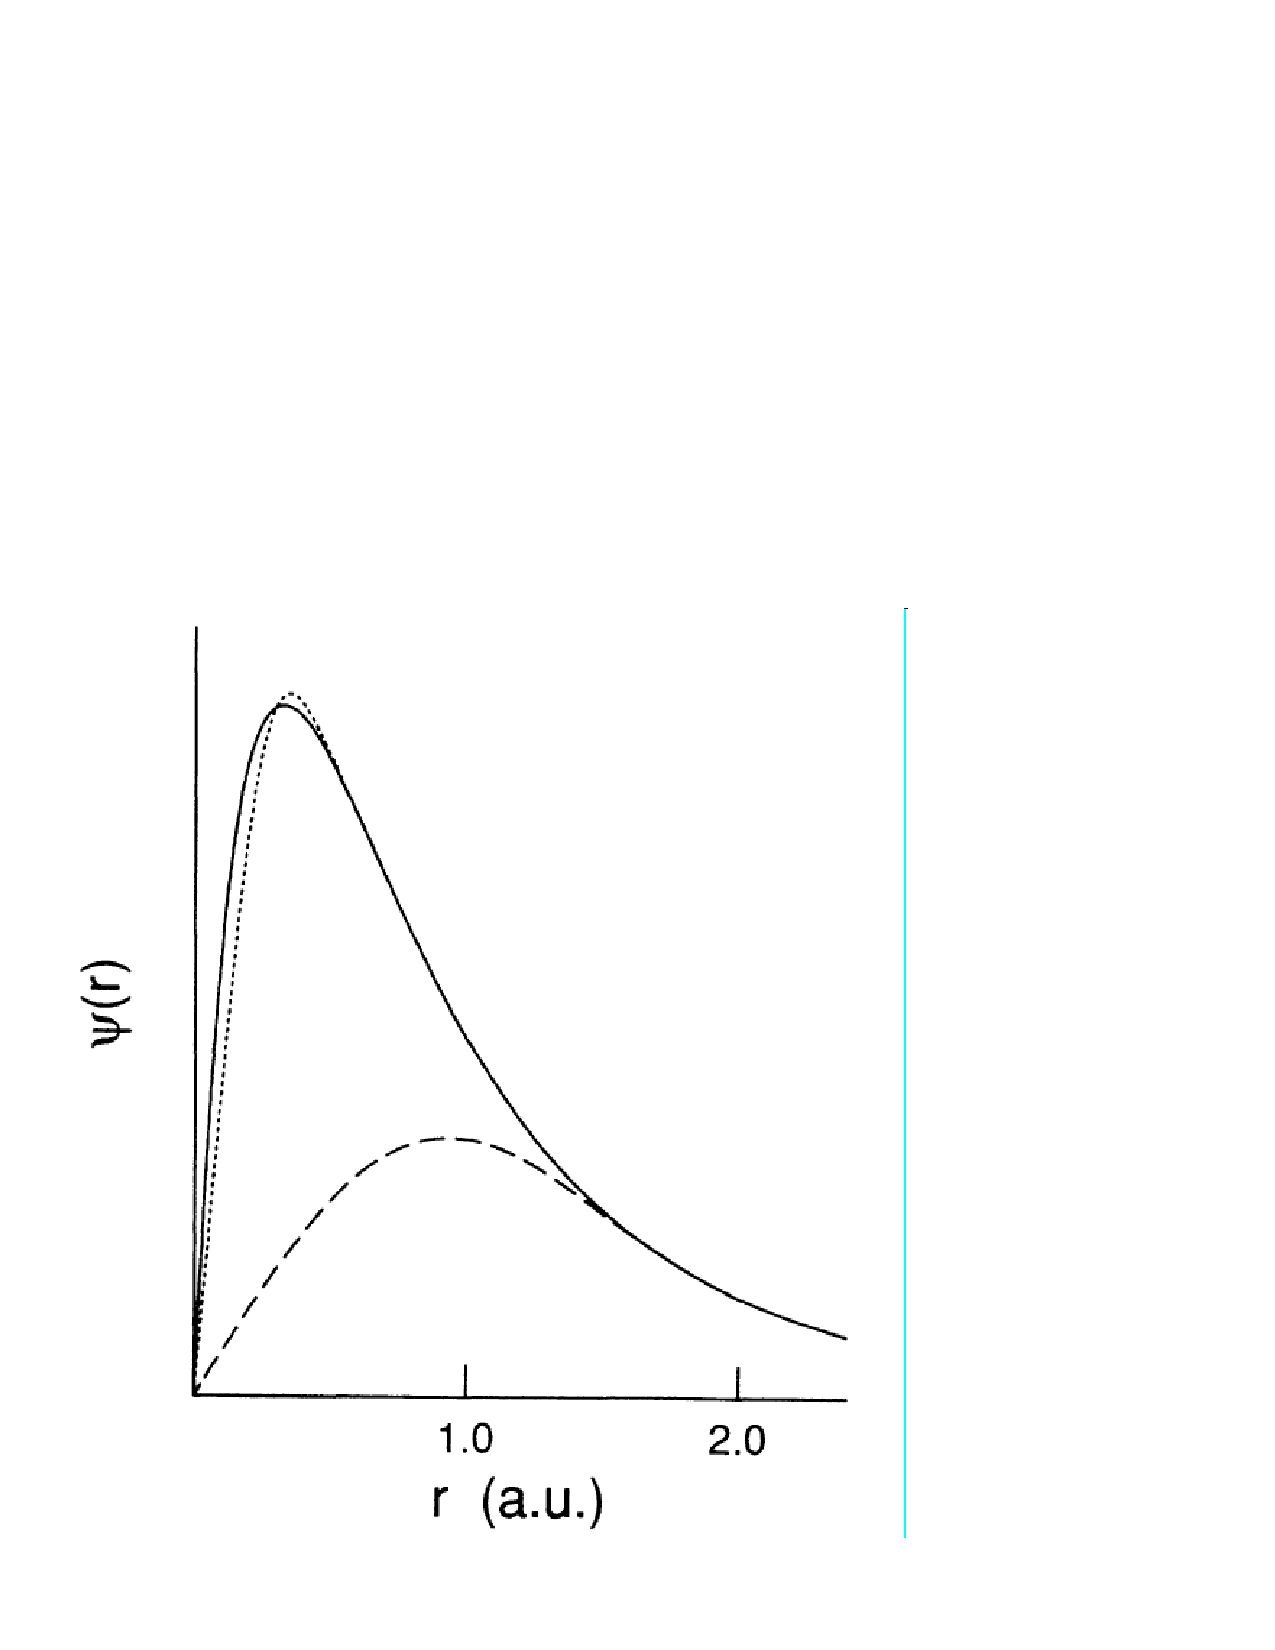
\includegraphics[height=1.35in,width=1.40in,viewport=30 55 415 500,clip]{Figures/Norm-US-wave.pdf}
\caption{\small \textrm{Oxygen 2} \textit{p} \textrm{radical wave function (solid), NC-pseudo-wave (dottde) and US-pseudo-wave (dashed).}}%(与文献\cite{EPJB33-47_2003}图1对比)
\label{Norm-US-wave}
\end{figure}
}

\frame
{
	\frametitle{补偿电荷的表示}
	\textcolor{magenta}{超软赝势的核心思想}:~解除模守恒条件,通过引入补偿电荷$\hat n$保持了赝势的可移植性
	
	一般要求局域在缀加区(\textrm{Augmentation region}),补偿电荷表示为
	$$\hat n=\sum_R\hat n_R$$
	其中$\hat n_R$是单个原子截断区间的补偿电荷,可以表示为广义的\textrm{Gaussian}函数的求和
	$$\hat n_R(r)=\sum_{L=(l,m)}g_{RL}(r)Q_{RL}$$
	其中$g_{RL}(r)$表示为
	$$g_{RL}(r)=C_l|r-R|^lY_L(r-R)\mathrm{e}^{-(|r-R|/r_c)^2}$$
	系数$C_l$是归一化系数,由条件
	$\int\mathrm{d}rr^lY_L(r)g_L(r)=1$
	确定

	$Q_{RL}$是补偿电荷要满足的多极矩
	$$Q_{RL}=\int\mathrm{d}r|r-R|^l\big[n_R(r)+n_R^Z(r)-\tilde n_R(r)\big]Y_L^{\ast}(r-R)$$
}

\section{\rm{PAW~}方法}
\subsection{\rm{PAW}方法的基本思想}
\frame
{
	\frametitle{\textrm{PAW}方法的基本思想}
	\vspace{10pt}
\begin{figure}[h!]
\centering
\includegraphics[height=1.8in,width=4.in,viewport=30 210 570 440,clip]{Figures/PAW_projector.eps}
\caption{\small \textrm{The analysis of PAW basic function.}}%(与文献\cite{EPJB33-47_2003}图1对比)
\label{PAW_baisc}
\end{figure}
}

\frame
{
	\frametitle{\textrm{PAW}方法概要}
\begin{itemize}
	\item 与芯层态正交的全部价电子构成的\textrm{Hilbert}空间%,价电子彼此的正交使得波函数在\textrm{Muffin-tin}球内振荡
	\item 作\textcolor{red}{线性空间变换},全电子波函数$|\Psi\rangle$与赝波函数$|\tilde\Psi\rangle$满足:
		$$|\Psi\rangle=\mathbf{\tau|}\tilde\Psi\rangle$$
%	$$\tau=\mathbf{1}+\sum_{\mathrm R}\hat\tau_{\mathrm R}$$
	\item 在原子核附近的$r_c$范围内,波函数用原子分波函数展开:
	$$|\Psi\rangle=|\tilde\Psi\rangle+\sum_i(|\phi_i\rangle-|\tilde\phi_i\rangle)\langle\tilde p_i|\tilde\Psi\rangle$$
	\item 在$r_c$外$|\tilde\Psi\rangle$与$|\Psi\rangle$变换前后保持不变,因此线性变换$\mathbf{\tau}$可表示为:
	$$\mathbf{\tau}=\mathbf{1}+\sum_i(|\phi_i\rangle-|\tilde\phi_i\rangle)\langle\tilde p_i|$$
\end{itemize}
其中$|\tilde p_i\rangle$是\textrm{MT}球内的投影函数\\
$i$表示原子位置$\vec R$、原子轨道($l,m$)和能级$\epsilon_k$的指标。
}

\frame
{
\frametitle{\textrm{PAW}方法的基本思想}
	在赝波函数$|\tilde\Psi\rangle$表象下,算符期望值计算满足$$\langle A \rangle=\langle\Psi|\mathbf{A}|\Psi\rangle=\langle\tilde\Psi|\mathbf{\tau}^{\dag}\mathbf{A}\mathbf{\tau}|\tilde\Psi\rangle=\langle\tilde\Psi|\tilde{\mathrm{A}}|\tilde\Psi\rangle$$
\begin{itemize}
	\item 一般赝算符$\tilde A$表示为
		$$\tilde A=\mathbf{A}+\sum_i|\tilde p_i\rangle(\langle\phi_i|\mathbf{A}|\phi_i\rangle-\langle\tilde\phi_i|\mathbf{A}|\tilde\phi_i\rangle)\langle\tilde p_i|$$
	\item 赝重叠算符$\tilde O$表示为
		$$\tilde O=\mathbf{1}+\sum_i|\tilde p_i\rangle(\langle\phi_i|\phi_i\rangle-\langle\tilde\phi_i|\tilde\phi_i\rangle)\langle\tilde p_i|$$
\end{itemize}
}

\frame
{
\frametitle{\textrm{PAW}方法密度和总能计算}
在\textrm{PAW}框架下,将密度算符$|\vec r\rangle\langle\vec r|$代入,可知密度表达式为
$$n(\vec r)=\tilde n(\vec r)+n^1(\vec r)-\tilde n^1(\vec r)$$
这里
$$\tilde n(\vec r)=\sum_nf_n\langle\tilde\Psi_n|\vec r\rangle\langle\vec r|\tilde\Psi_n\rangle$$ 
$$n^1(\vec r)=\sum_{n,(i,j)}f_n\langle\tilde\Psi_n|\tilde p_i\rangle\langle\phi_i|\vec r\rangle\langle\vec r|\phi_j\rangle\langle\tilde p_j|\tilde\Psi_n\rangle$$
$$\tilde n^1(\vec r)=\sum_{n,(i,j)}f_n\langle\tilde\Psi_n|\tilde p_i\rangle\langle\tilde\phi_i|\vec r\rangle\langle\vec r|\tilde\phi_j\rangle\langle\tilde p_j|\tilde\Psi_n\rangle$$
总能量泛函
$$E=\tilde E+E^1-\tilde E^1$$
}

\frame
{
	\frametitle{重叠矩阵和\textrm{Hamiltonian}矩阵}
重叠算符:
$$\tilde O=1+\sum_{i,j}|\tilde p_i\rangle\bigg[\langle\phi_i|\phi_j\rangle-\langle\tilde\phi_i|\tilde\phi_j\rangle\bigg]\langle\tilde p_j|$$
\textrm{Hamilitonian}算符:
%\begin{itemize}
%	\item 动能算符:
%		$$\tilde T=-\dfrac12\nabla^2+\sum_{i,j}|\tilde p_i\rangle[\langle\phi_i|-\dfrac12\nabla^2|\phi_j\rangle-\langle\tilde\phi_i|-\dfrac12\nabla^2|\tilde\phi_j\rangle]\langle\tilde p_j|$$
%	\item 完全势\textrm{(full-potential)}算符:
%$$v(\vec r)=\tilde v(\vec r)+v^1(\vec r)-\tilde v^1(\vec r)$$
%	\item \textrm{Hamilton}算符:
\begin{displaymath}
	\begin{aligned}
		\tilde H=&-\dfrac12\nabla^2+\tilde v+\sum_{i,j}|\tilde p_i\rangle\bigg[\langle\phi_i|-\dfrac12\nabla^2+v^1|\phi_j\rangle\\
			&-\langle\tilde\phi_i|-\dfrac12\nabla^2+\tilde v^1|\tilde\phi_j\rangle\bigg]\langle\tilde p_j| 
	\end{aligned}
\end{displaymath}
%\end{itemize}
	完整的势函数\textrm{(full-potential)}算符:
$$v(\vec r)=\tilde v(\vec r)+v^1(\vec r)-\tilde v^1(\vec r)$$
因此可以有
$$\left.\dfrac{\partial E[\tilde\Psi, R]}{\partial\langle\tilde\Psi_n|}\right|_R=\tilde H|\tilde\Psi_n\rangle f_n$$
}

%\subsection{\rm{PAW}的实现}
%\frame
%{
%%	\frametitle{\textrm{PAW}原子数据集}
%	\frametitle{\textrm{PAW Augmentation}}
%\begin{figure}[h!]
%\centering
%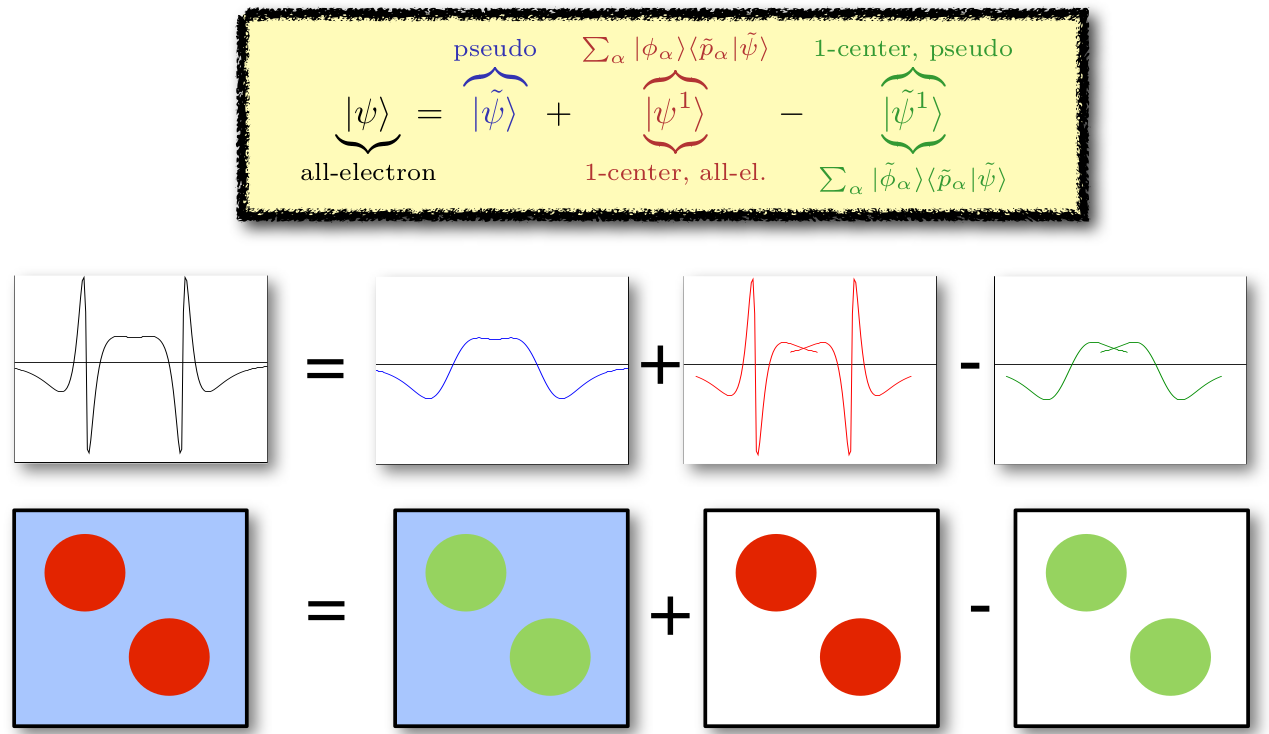
\includegraphics[height=2.3in,width=4.0in,viewport=0 0 1280 745,clip]{Figures/PAW-baseset.png}
%\caption{\small \textrm{The Augmentation of PAW.}}%(与文献\cite{EPJB33-47_2003}图1对比)
%\label{PAW_baiseset}
%\end{figure}
%}

%\frame
%{
%	\frametitle{\textrm{PAW Augmentation}}
%\begin{figure}[h!]
%\centering
%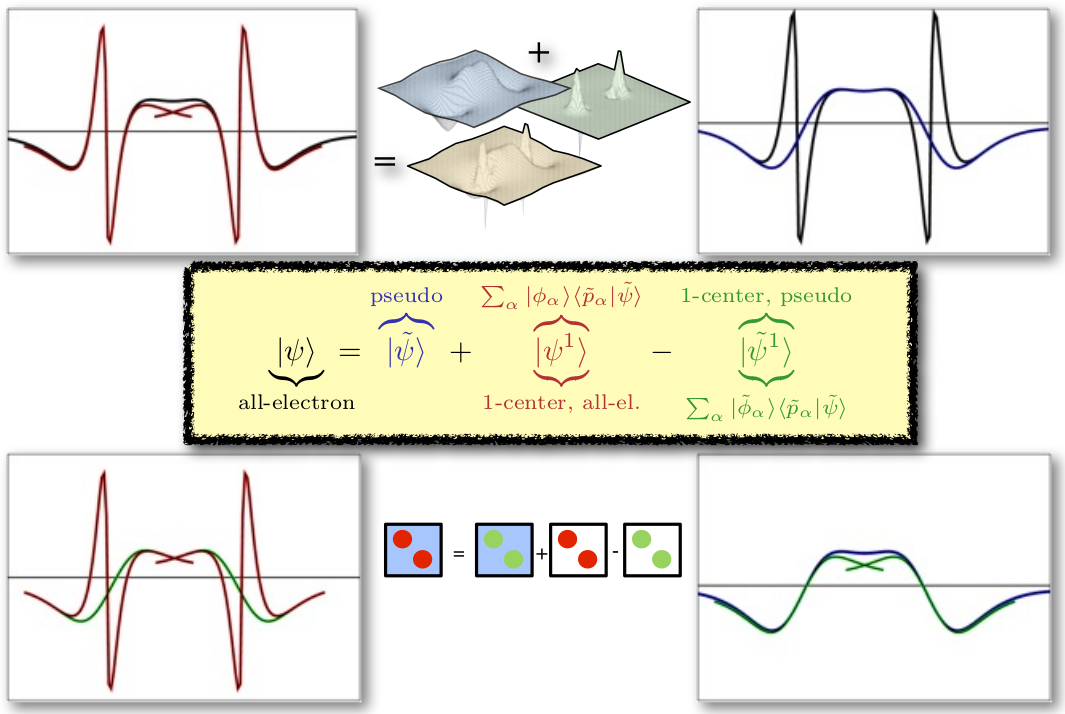
\includegraphics[height=2.3in,width=4.0in,viewport=0 0 1100 745,clip]{Figures/PAW-projector.png}
%\caption{\small \textrm{The projector of PAW.}}%(与文献\cite{EPJB33-47_2003}图1对比)
%\label{PAW_projector}
%\end{figure}
%}

\subsection{\rm{VASP~}软件中\rm{PAW~}实现}
\frame
{
%	\frametitle{\textrm{PAW}原子数据集}
	\frametitle{\textrm{PAW Augmentation}}
\begin{figure}[h!]
\centering
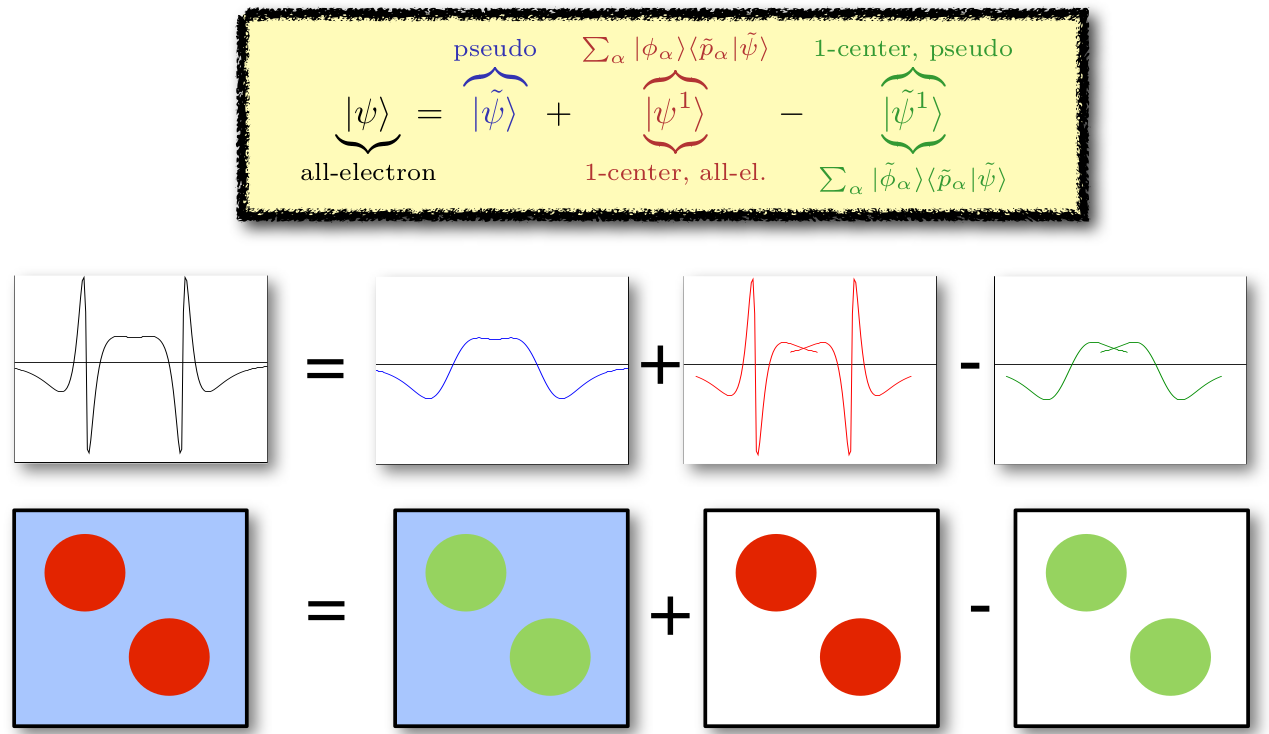
\includegraphics[height=2.3in,width=4.0in,viewport=0 0 1280 745,clip]{Figures/PAW-baseset.png}
\caption{\small \textrm{The Augmentation of PAW.}}%(与文献\cite{EPJB33-47_2003}图1对比)
\label{PAW_baiseset}
\end{figure}
}

%\frame
%{
%	\frametitle{\textrm{PAW Augmentation}}
%\begin{figure}[h!]
%\centering
%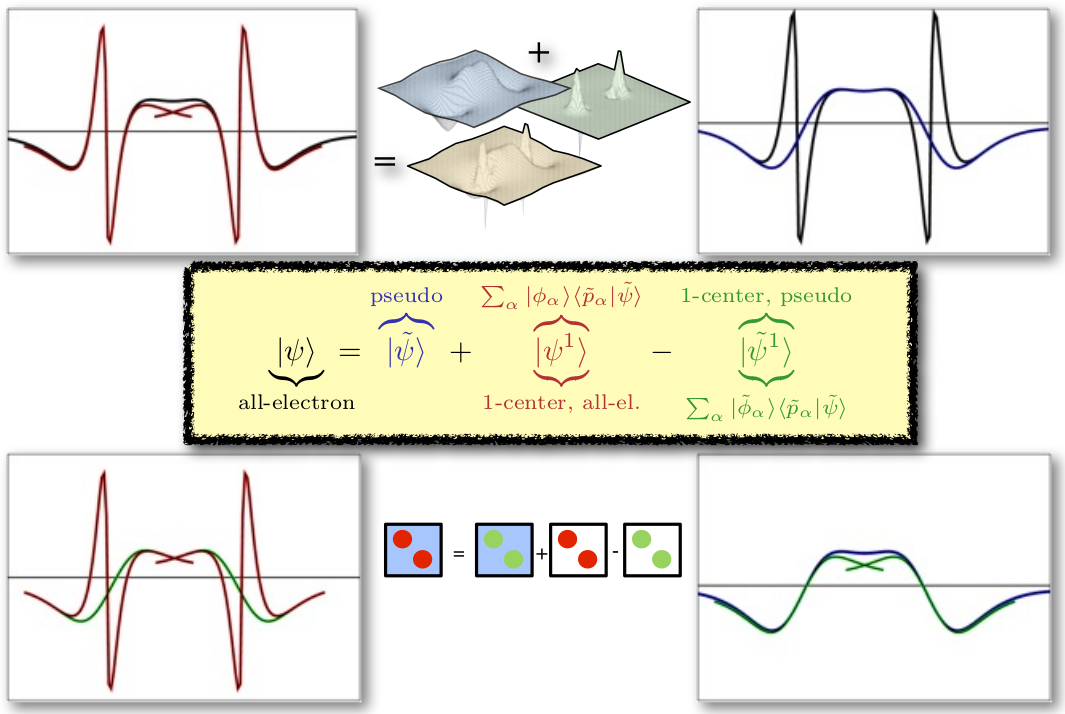
\includegraphics[height=2.3in,width=4.0in,viewport=0 0 1100 745,clip]{Figures/PAW-projector.png}
%\caption{\small \textrm{The projector of PAW.}}%(与文献\cite{EPJB33-47_2003}图1对比)
%\label{PAW_projector}
%\end{figure}
%}

\frame
{
\frametitle{电荷密度的重新分解}
\textrm{PAW}方法提出后有很长一段时间没有能够得到广泛应用,直到\textrm{G. Kresse}等将\textrm{Bl\"ochl}的原始方案中电荷密度计算方案重新组合后,明确了\textrm{PAW}方法与\textrm{USPP}方法的内在联系。
\begin{itemize}
	\item 芯层电荷与核电荷构成离子实电荷:$n_{Zc}=n_Z+n_c$
	\item 赝离子实电荷的构造$$\int_{\Omega_c}n_{Zc}(\vec r)\mathrm{d}^3\vec r=\int_{\Omega_c}\tilde n_{Zc}(\vec r)\mathrm{d}^3\vec r$$
\end{itemize}
在此基础上,\textrm{Bl\"ochl}方案中的电荷可以分解为:
\begin{displaymath}
	\begin{aligned}
		n_T=n+n_{Zc}\equiv&\underbrace{(\tilde n+\hat n+\tilde n_{Zc})}\\
				 		&\quad\qquad\tilde n_T\\
				  &+\underbrace{(n^1+\hat n+n_{Zc})}-\underbrace{(\tilde n^1+\hat n+\tilde n_{Zc})}\\
				                  &\quad\qquad n_T^1\qquad\qquad\qquad\tilde n_T^1
	\end{aligned}
\end{displaymath}
\textcolor{red}{注意}:\textrm{G. Kresse}方案中补偿电荷$\hat n$局域在每个缀加球内。
}

\frame
{
	\frametitle{\textrm{Hartree~}势的分解}
\begin{displaymath}
	\begin{aligned}
		\dfrac12(n_T)(n_T)=&\dfrac12(\tilde n_T)(\tilde n_T)+(n_T^1-\tilde n_T^1)(\tilde n_T)\\
				&+\dfrac12(n_T^1-\tilde n_T^1)(n_T^1-\tilde n_T)
	\end{aligned}
\end{displaymath}
这里$$(a)(b)=\int\mathrm{d}\vec r\mathrm{d}\vec r^{\prime}\dfrac{a(\vec r)b(\vec r\,^{\prime})}{|\vec r-\vec r\,^{\prime}|}$$
\textcolor{red}{近似}:$\tilde n_T$用$\tilde n_T^1$替换:
\begin{displaymath}
	\dfrac12(n_T)(n_T)=\dfrac12(\tilde n_T)(\tilde n_T)-\dfrac12\overline{(n_T^1(\tilde n_T^1)}+\dfrac12\overline{(n_T^1)(n_T^1)}
\end{displaymath}
}

\frame
{
\frametitle{交换-相关能泛函的处理}
由于交换-相关能泛函是非线性的,\textrm{G. Kresse}方案中电荷密度分解为
\begin{displaymath}
	n_c+n=(\tilde n+\hat n+\tilde n_c)+(n^1+n_c)-(\tilde n^1+\hat n+\tilde n_c)
\end{displaymath}
原始的\textrm{Bl\"ochl}方案中电荷分解为
\begin{displaymath}
	n_c+n=(\tilde n)+(n^1+n_c)-(\tilde n^1)
\end{displaymath}
\textcolor{blue}{两种不同的电荷密度分解方案根源}:\\\textrm{G. Kresse}方案中赝离子实电荷$\tilde n_{Zc}$与\textrm{Bl\"ochl}方案中$\tilde n_c$的约束条件不同!
\begin{displaymath}
	E_{\mathrm{XC}}[\tilde n+\hat n+\tilde n_c]+\overline{E_{\mathrm{XC}}[n^1+n_c]}-\overline{E_{\mathrm{XC}}[\tilde n^1+\hat n+\tilde n_c]}
\end{displaymath}
}

\frame
{
	\frametitle{总能量表达式}
	根据总能量表达式$$E=\tilde E+E^1-\tilde E^1$$其中
	\begin{displaymath}
		\begin{aligned}
			\tilde E=&\sum_nf_n\langle\tilde\Psi_n|-\frac12\nabla^2|\tilde\Psi_n\rangle+E_{\mathrm{XC}}[\tilde n+\hat n+\tilde n_c]+E_H[\tilde n+\hat n]\\
			&+\int v_H[\tilde n_{Zc}][\tilde n(\vec r)+\hat n(\vec r)]\mathrm{d}\vec r+U(\vec R,Z_{\mathrm{ion}})\\
			\tilde E^1=&\sum_{(i,j)}\rho_{ij}\langle\tilde\phi_i|-\frac12\nabla^2|\tilde\phi_j\rangle+\overline{E_{\mathrm{XC}}[\tilde n^1+\hat n+\tilde n_c]}+\overline{E_H[\tilde n^1+\hat n]}\\
			&+\int_{\Omega_r}v_H[\tilde n_{Zc}][\tilde n^1(\vec r)+\hat n(\vec r)]\mathrm{d}\vec r
		\end{aligned}
	\end{displaymath}
}

\frame
{
	\frametitle{总能量表达式}
	\begin{displaymath}
		\begin{aligned}
			E^1=&\sum_{(i,j)}\rho_{ij}\langle\phi_i|-\frac12\nabla^2|\phi_j\rangle+\overline{E_{\mathrm{XC}}[n^1+n_c]}+\overline{E_H[n^1]}\\
			&+\int_{\Omega_r}v_H[n_{Zc}]n^1(\vec r)\mathrm{d}\vec r
		\end{aligned}
	\end{displaymath}
	$v_H$是电荷密度$n$产生的静电势
	$$v_H[n](\vec r)=\int\dfrac{n(\vec r\,^{\prime})}{|\vec r-\vec r\,^{\prime}|}\mathrm{d}\vec r\,^{\prime}$$
	$E_H[n]$是对应的静电能
	$$E_H[n]=\dfrac12(n)(n)=\dfrac12\int\mathrm{d}\vec r\mathrm{d}\vec r\,^{\prime}\dfrac{n(\vec r)n(\vec r\,^{\prime})}{|\vec r-\vec r\,^{\prime}|}$$ 
	$U(\vec R,Z_{\mathrm{ion}})$\textcolor{blue}{由\textrm{Ewald}求和计算}
}

\frame
{
	\frametitle{补充电荷的构造}
	根据约束条件
	\begin{displaymath}
		\int_{\Omega_c}(n^1-\tilde n^1-\hat n)|\vec r-\vec R|^lY_{lm}^{\ast}(\widehat{\vec r-\vec R})\mathrm{d}\vec r=0
	\end{displaymath}
	定义电荷密度差
	\begin{displaymath}
		Q_{ij}(\vec r)=\phi_i^{\ast}(\vec r)\phi_j(\vec r)-\tilde\phi_i^{\ast}(\vec r)\tilde\phi_j(\vec r)
	\end{displaymath}
	电荷密度差的多极矩为
	\begin{displaymath}
		q_{ij}^L(\vec r)=\int_{\Omega_r}Q_{ij}(\vec r)|\vec r-\vec R|^lY_{lm}^{\ast}(\widehat{\vec r-\vec R})\mathrm{d}\vec r
	\end{displaymath}
	因此,补充电荷的计算为:
	\begin{displaymath}
		\begin{aligned}
			\hat n=\sum_{(i,j),L}\sum_n f_n\langle\tilde\Psi_n|\tilde p_i\rangle\langle\tilde p_j|\Psi_n\rangle\hat Q_{ij}^L(\vec r)\\
			\hat Q_{ij}^L(\vec r)=q_{ij}^Lg_l(|\vec r-\vec R|)Y_{lm}(\widehat{\vec r-\vec R})
		\end{aligned}
	\end{displaymath}
}

\frame
{
	\frametitle{重叠矩阵和\textrm{Hamiltonian~}的构造}
重叠矩阵
	\begin{displaymath}
		\langle\tilde\Psi_n|\mathbf{S}|\tilde\Psi_m\rangle=\delta_{nm}
	\end{displaymath}
	其中重叠矩阵$$S[\{\mathbf{R}\}]=1+\sum_i|\tilde p_i\rangle q_{ij}\langle\tilde p_j|$$
	而$$q_{ij}=\langle\phi_i|\phi_j\rangle-\langle\tilde\phi_i|\tilde\phi_j\rangle$$
	\textrm{Hamiltonian}的计算
	\begin{displaymath}
		H[\rho,\{\mathbf{R}\}]=-\dfrac12\nabla^2+\tilde v_{eff}+\sum_{(i,j)}|\tilde p_i\rangle(\hat D_{ij}+D_{ij}^1-\tilde D_{ij}^1)\langle\tilde p_j|	
	\end{displaymath}
	$$\tilde v_{eff}=v_H[\tilde n+\hat n+\tilde n_{Zc}]+v_{\mathrm{XC}}[\tilde n+\hat n+\tilde n_{Zc}]$$
}

\frame
{
	\frametitle{重叠矩阵和\textrm{Hamiltonian~}的构造}
	$$\hat D_{ij}=\dfrac{\partial\tilde E}{\partial\rho_{ij}}=\int\dfrac{\delta\tilde E}{\delta\hat n(\vec  r)}\dfrac{\partial\hat n(\vec r)}{\partial\rho_{ij}}\mathrm{d}\vec r=\sum_{L}\int\tilde v_{eff}\hat Q_{ij}^L(\vec r)\mathrm{d}\vec r$$
	$$D_{ij}^1=\dfrac{\partial E^1}{\partial\rho_{ij}}=\langle\phi_i|-\dfrac12\nabla^2+v_{eff}^1|\phi_j\rangle$$
	其中$$v_{eff}^1[n^1]=v_H[n^1+n_{Zc}]+v_{\mathrm{XC}}[n^1+n_c]$$
	$$\tilde D_{ij}^1=\dfrac{\partial\tilde E^1}{\partial\rho_{ij}}=\langle\tilde\phi_i|-\dfrac12\nabla^2+\tilde v_{eff}^1|\tilde\phi_j\rangle+\sum_L\int_{\Omega_r}\mathrm{d}\vec r\tilde v_{eff}^1(\vec r)\hat Q_{ij}^L$$
	其中$$\tilde v_{eff}^1[\tilde n^1]=v_H[\tilde n^1+\hat n+\tilde n_{Zc}]+v_{\mathrm{XC}}[\tilde n^1+\hat n+\tilde n_c]$$
}

\frame
{
	\frametitle{\textrm{Double counting correlations}}
	能带计算中,总能量可通过\textrm{Kohn-Sham}本征值求和扣除\textrm{Double counting}计算更方便,其中修正项
	\begin{displaymath}
		\begin{aligned}
			\tilde E_{dc}=&-E_H[\tilde n+\hat n]+E_{\mathrm{XC}}[\tilde n+\hat n+\tilde n_c]\\
			&-\int v_{\mathrm{XC}}[\tilde n+\hat n+\tilde n_c](\tilde n+\hat n)\mathrm{d}\vec r\\
			E_{dc}^1=-\overline{E_H[n^1]}&+\overline{E_{\mathrm{XC}}[n^1+n_c]}-\int_{\Omega_r}v_{\mathrm{XC}}[n^1+n_c]n^1\mathrm{d}\vec r\\
			\tilde E_{dc}^1=&-\overline{E_H[\tilde n^1+\hat n]}+\overline{E_{\mathrm{XC}}[\tilde n^1+\hat n+\tilde n_c]}\\
			&-\int v_{\mathrm{XC}}[\tilde n^1+\hat n+\tilde n_c](\tilde n^1+\hat n)\mathrm{d}\vec r
		\end{aligned}
	\end{displaymath}
	因此总能量的计算表达式是
	$$E=\sum_nf_n\langle\tilde\Psi_n|H|\tilde\Psi_n\rangle+\tilde E_{dc}+E_{dc}^1-\tilde E_{dc}^1+U(\vec R,Z_{\mathrm{ion}})$$
}

\frame
{
	\frametitle{双网格技术}
\begin{figure}[h!]
	\vspace{-0.2in}
\centering
%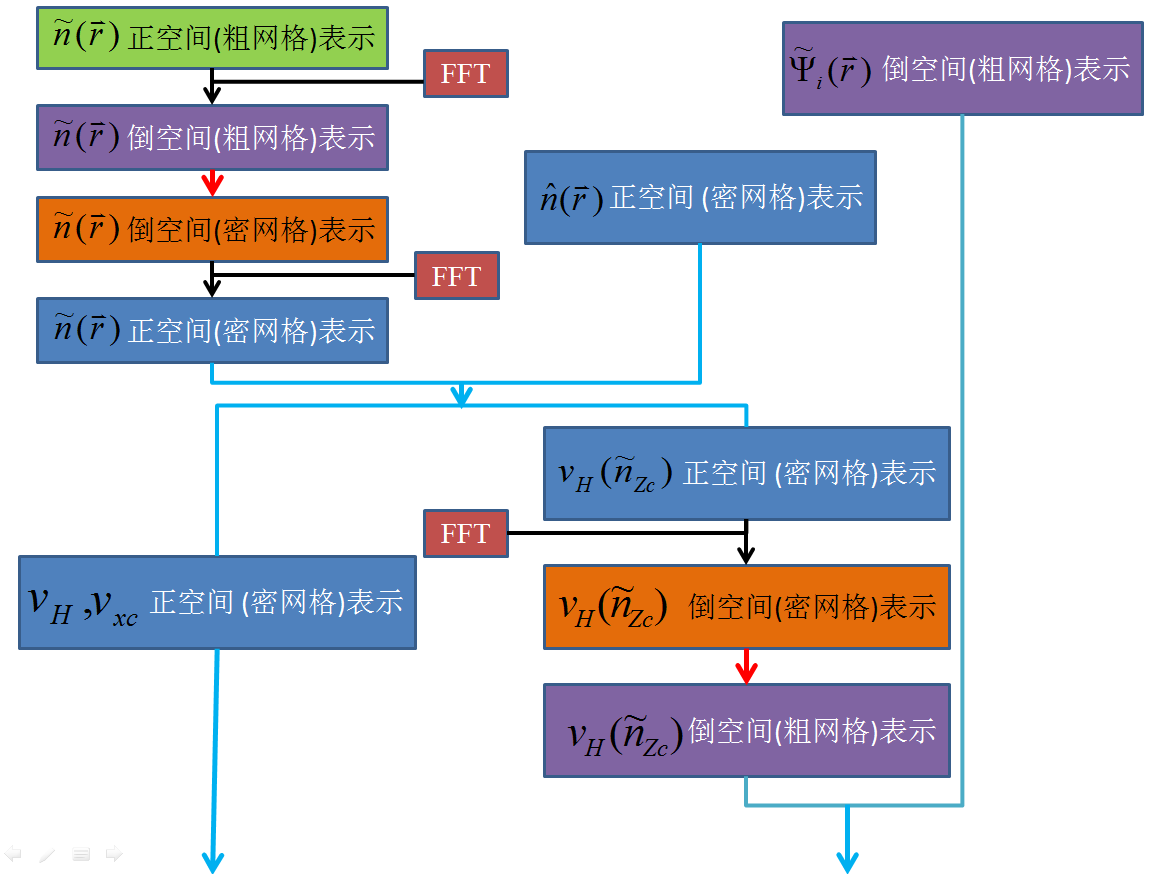
\includegraphics[height=2.7in,width=4.0in,viewport=0 0 1180 875,clip]{Figures/dual_grid.png}
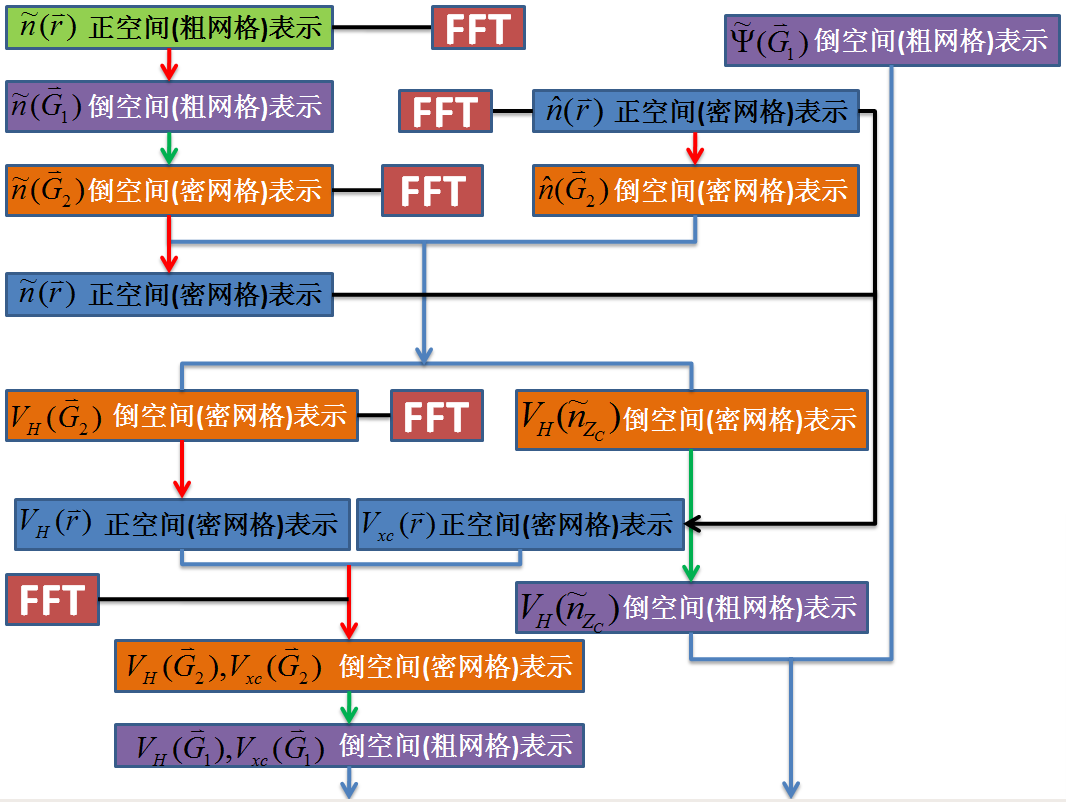
\includegraphics[height=2.7in,width=4.0in,viewport=0 0 800 600,clip]{Figures/dual_grid-2.png}
\caption{\small \textrm{The Schematic description of the dual grid technique.}}%(与文献\cite{EPJB33-47_2003}图1对比)
\label{PAW_baiseset}
\end{figure} 
}

\frame
{
	\frametitle{双网格技术}
\begin{figure}[h!]
	\vspace{-0.2in}
\centering
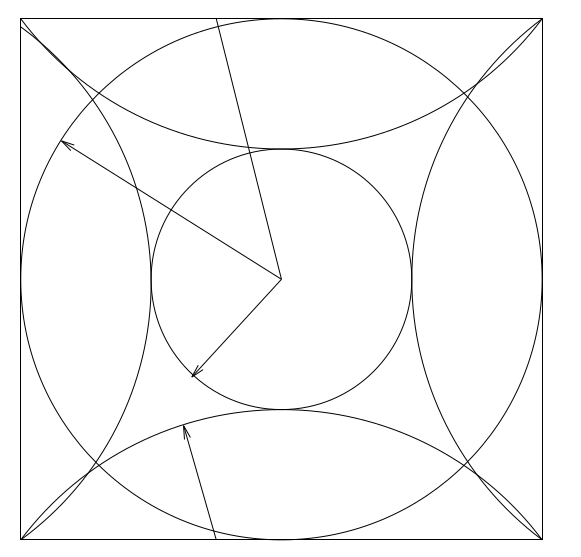
\includegraphics[height=2.3in,width=2.3in,viewport=0 0 420 420,clip]{Figures/VASP_G_max.png}
\caption{\fontsize{5.2pt}{3.9pt}\selectfont{\textrm{The small sphere contains all plane waves included in the basis set $\vec G<\vec G_\mathrm{cut}$. The charge density contains components up to $2\vec G$ cut (second sphere), and the acceleration a components up to $3\vec G$ cut , which are reflected in (third sphere) because of the finite size of the FFT-mesh. Nevertheless the components a $\vec G$ with $|\vec G|<\vec G$ cut are correct i.e. the small sphere does not intersect with the third large sphere.}}}%(与文献\cite{EPJB33-47_2003}图1对比)
\label{VASP_G_max}
\end{figure} 
}

%\frame
%{
%\frametitle{发展统一理论框架下的材料计算程序}
%\begin{itemize}
%	\item
%\end{itemize}
%}

\subsection{\rm{PAW}方法与\rm{US-PP}的关系}
\frame
{
	\frametitle{\textrm{PAW}与\textrm{US-PP}近似}
	\textrm{G. Kresse}指出只要总能量表达式中$E^1$和$\tilde E^1$在原子构象附近作线性化即可得到\textrm{US-PP}的表达式。
	
	如果原子构象由占据数$\rho_{ij}^a$、电荷密度分布$n_a^1$、$\tilde n_a^1$和$\hat n_a$确定,$E^1$中的\textcolor{blue}{\underline{\textrm{Hartree}能和交换-相关能项}}在$n_a^1$附近线性化得
	\begin{displaymath}
		E_{\mathrm{XC}}(\textcolor{red}{n_a^1+n_c})+E_H(\textcolor{red}{n_a^1})+\int(v_{\mathrm{XC}}[n_a^1+n_c]+v_H[n_a^1])\underline{\textcolor{red}{[n^1(\vec r)-n_a^1(\vec r)]}\mathrm{d}\vec r}
	\end{displaymath}
	在\textrm{PAW}方法中,电子密度$n^1(\vec r)$%和$\tilde n^1(\vec r)$
	的表达式
	\begin{displaymath}
		\begin{aligned}
			n^1(\vec2 r)=&\sum_{(i,j)}\rho_{ij}\langle\phi_i|\vec r\rangle\langle\vec r|\phi_j\rangle\\
	%		\tilde n^1(\vec r)=&\sum_{(i,j)}\rho_{ij}\langle\tilde\phi_i|\vec r\rangle\langle\vec r|\tilde\phi_j\rangle 
		\end{aligned}
	\end{displaymath}
	因此,\textrm{Hartree}能和交换-相关能项为
	$$\textcolor{blue}{C}+\sum_{(i,j)}\rho_{ij}\langle\phi_i|\textcolor{red}{v_{\mathrm{XC}}[n_a^1+n_c]+v_H[n_a^1]}|\phi_j\rangle$$
	这里\textcolor{blue}{\textrm{C}}是常数
}

\frame
{
	\frametitle{\textrm{PAW}与\textrm{US-PP}近似}
	因此$E^1$用占据数$\rho_{ij}$近似到一阶可有
	\begin{displaymath}
		E^1\approx\textcolor{blue}{C}+\sum_{(i,j)}\langle\phi_i|-\frac12\nabla^2+v_{eff}^a|\phi_j\rangle
	\end{displaymath}
	其中
	\begin{displaymath}
		v_{eff}^a=\textcolor{red}{v_H[n_a^1+}\textcolor{blue}{n_{Zc}}\textcolor{red}{]+v_{\mathrm{XC}}[n_a^1+n_c]}
	\end{displaymath}
	这里\textcolor{red}{$v_{eff}^a$}是\textcolor{blue}{原子构象下的全电子有效势}

	类似地可有
	\begin{displaymath}
		\tilde E^1\approx\textcolor{blue}{\tilde C}+\sum_{(i,j)}\left[\langle\tilde\phi_i|-\frac12\nabla^2+\tilde v_{eff}^a|\tilde\phi_j\rangle+\underline{\int\tilde Q_{ij}^L(\vec r)\tilde v_{eff}^a(\vec r)\mathrm{d}\vec r}\right]
	\end{displaymath}
	其中$$\tilde v_{eff}^a=v_H[\tilde n_a^1+\textcolor{blue}{\hat n_a}+\tilde n_{Zc}]+v_{\mathrm{XC}}[\tilde n_a^1+\textcolor{blue}{\hat n_a}+\tilde n_c]$$
	这里\textcolor{red}{$\tilde v_{eff}^a$}是\textcolor{blue}{原子构象下的局域原子赝势}
}

\frame
{
	\frametitle{\textrm{PAW}与\textrm{US-PP}近似}
	在此近似下,包含$\tilde E$可得体系总能量$E$:
	\begin{displaymath}
		\begin{aligned}
			E=&\sum_nf_n\langle\tilde\Psi_n|-\frac12\nabla^2+\sum_{(ij)}|\tilde p_i\rangle\langle\tilde p_j|G_{ij}^{\mathrm{US}}|\tilde\Psi_n\rangle\\
			&+E_{\mathrm{XC}}[\tilde n+\hat n+\tilde n_c]+E_H[\tilde n+\hat n]\\
			&+\int v_H[\tilde n_{Zc}][\tilde n(\vec r)+\hat n(\vec r)]\mathrm{d}\vec r+U(\vec R,Z_{\mathrm{ion}})
		\end{aligned}
	\end{displaymath}
	其中
	\begin{displaymath}
		\begin{aligned}
			G_{ij}^{\mathrm{US}}=&\langle\phi_i|-\frac12\nabla^2+v_{eff}^a|\phi_j\rangle-\langle\tilde\phi_i|-\frac12\nabla^2+\tilde v_{eff}^a|\tilde\phi_j\rangle\\
			&-\int\hat Q_{ij}^L(\vec r)\tilde v_{eff}^a(\vec r)\mathrm{d}\vec r
		\end{aligned}
	\end{displaymath}
	\textcolor{red}{当补偿电荷$\hat n$用\textrm{US-PP}方案的赝化补偿电荷表示时,$E\rightarrow E_{\mathrm{tot}}$}
}

\frame
{
	\frametitle{\textrm{PAW}与\textrm{US-PP}近似}
	在$G_{ij}^{\mathrm{US}}$中,
	\begin{displaymath}
		\begin{aligned}
			&\textcolor{blue}{\langle\phi_i|-\frac12\nabla^2+v_{eff}^a|\phi_j\rangle-\langle\tilde\phi_i|-\frac12\nabla^2+\tilde v_{eff}^a|\tilde\phi_j\rangle}\\
			\rightarrow&\textcolor{red}{D_{nm}=B_{nm}+\varepsilon_mq_{nm}}
		\end{aligned}
	\end{displaymath}
	\begin{displaymath}
		\textcolor{blue}{\int\hat Q_{ij}^L(\vec r)\tilde v_{eff}^a(\vec r)\mathrm{d}\vec r}\rightarrow\textcolor{red}{D_{nm}^{(0)}=D_{nm}-\int\mathrm{d}\vec r\,^{\prime}V_{loc}(\vec r\,^{\prime})n(\vec r\,^{\prime})}
	\end{displaymath}

	在\textrm{PAW}方法能量泛函中,如果缀加区补偿电荷$\hat n$满足$$\hat n=n^1-\tilde n^1$$
	并且如果满足$\tilde n_{Zc}=n_{Zc}$和$\tilde n_c=n_c$,则“在位”(\textrm{on-site})动能对总能的贡献
	\begin{displaymath}
		E^1-\tilde E^1=\sum_{(i,j)}\rho_{ij}\big(\langle\phi_i|-\frac12\nabla^2|\phi_j\rangle-\langle\tilde\phi_i|-\frac12\nabla^2|\tilde\phi_j\big)
	\end{displaymath}
}

\frame
{
	\frametitle{\textrm{PAW}与\textrm{US-PP}近似}
	\textcolor{red}{在这种极限情况下\textrm{PAW}与\textrm{US-PP}完全等价}

	在\textrm{US-PP}中,\textcolor{orange}{缀加函数}满足条件
	$$\hat Q_{ij}^L(\vec r)=Q_{ij}(\vec r)=\phi_i^{\ast}(\vec r)\phi_j(\vec r)-\tilde\phi_i^{\ast}(\vec r)\tilde\phi_j(\vec r)$$
	上述推导表明:~\textcolor{blue}{在\textrm{US-PP}方案中,可以通过提高\underline{赝化缀加函数}的精度,系统提升总能量的计算精度}
}

\section{迭代优化算法}
\frame
{
	\frametitle{\textrm{VASP~}计算流程}
\begin{figure}[h!]
	\vspace{-0.2in}
\centering
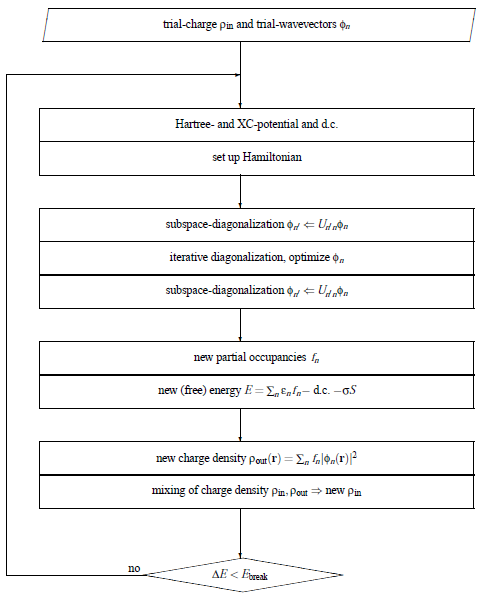
\includegraphics[height=2.1in,width=1.6in,viewport=0 0 480 630,clip]{Figures/VASP_procedure.png}
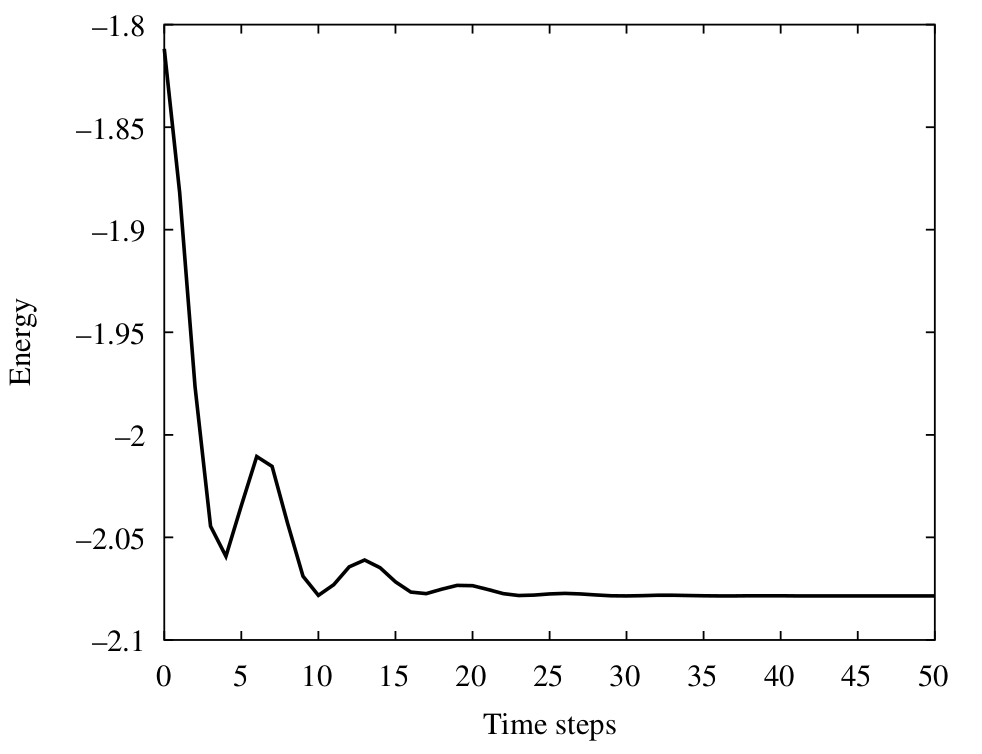
\includegraphics[height=2.1in,width=2.3in,viewport=0 0 740 600,clip]{Figures/Ab-initio-Ene.png}
\caption{\small \textrm{The Flow of calculation for the KS-ground states.}}%(与文献\cite{EPJB33-47_2003}图1对比)
\label{PAW_baiseset}
\end{figure} 
}

\subsection{第一原理分子动力学的基本思想}
%\subsection{电子态能量的最小化}
\frame
{
	\frametitle{电子态能量最小化}
	\textrm{Car-Parinello~}方法基本思想
	\begin{itemize}
		\item 只对原子核位置考虑受力$-\dfrac{\partial E_{\mathrm{tot}}}{\partial\vec R_n}$作用
		\item 电子结构是通过某种最小化方法确定能量泛函$E_{\mathrm{tot}}[\rho(\vec r)]$的极值得到,而非\textrm{Born-Oppenheimer}近似下的自洽迭代
		\item \textrm{Verlet}算法确定核位移过程中,并不要求在每一步核位移时,电子步充分弛豫到当前结构的基态
	\end{itemize}
	在\textrm{Car-Parinello}方法中,电子结构的计算变成经典的优化问题:~电子密度迭代过程中,约束条件下最小化问题
	\begin{itemize}
		\item 电子本征态波函数彼此正交约束下迭代对角化(内循环):\\
			\textcolor{blue}{子空间旋转}:~不同的正交化方法对迭代计算的影响
		\item 电荷密度混合过程中电荷数守恒约束(外循环)
			\begin{displaymath}
				\sum\limits_{j=0}^i a_j=1
			\end{displaymath}
	\end{itemize}
}


\frame
{
	\frametitle{能量泛函的直接优化}
	根据\textrm{Car-Parrinello~}定义的经典\textrm{Lagrangian~}量
	{\fontsize{9.0pt}{5.2pt}\selectfont
	\begin{displaymath}
		L(\{\psi_k\},\{\vec R_n\})=\frac{\mu}2\sum_k\dot{\psi}_k^2+\sum_n\frac{M_n}2\dot{\vec R}_n^2-E_{\mathrm{tot}}(\{\psi_k\},\{\vec R_n\})+\sum_{kl}\Lambda_{kl}\langle\psi_k|\psi_l\rangle
	\end{displaymath}}
	多粒子体系的\textrm{Euler-Lagrange~}运动方程可以表示为
	\begin{displaymath}
		\begin{aligned}
			\mu\ddot{\psi}_k=&-\dfrac{\partial E_{\mathrm{tot}}}{\partial\psi_k}+2\sum_i\Lambda_{kl}\psi_l(\vec r)\\
			M_n\ddot{\vec R}_n&=-\dfrac{\partial E_{\mathrm{tot}}}{\partial\vec R_n}+\sum_{kl}\Lambda_{kl}\dfrac{\partial\langle\psi_k|\psi_l\rangle}{\partial\vec R_n}
		\end{aligned}
	\end{displaymath}
	\textcolor{purple}{电子基态可以通过求解\textrm{Verlet~}运动方程得到}\\
	在\textrm{DFT~}框架下,有
	{\fontsize{9.0pt}{5.2pt}\selectfont
	\begin{displaymath}
		\psi_k(t+h)=2\psi_k(t)-\psi_k(t-h)-\dfrac{2h^2}{\mu}(H\psi_k-\sum_l\Lambda_{kl}\psi_l)
	\end{displaymath}}
%	该方程表明:~\textcolor{blue}{电子基态也可通过各种优化方法直接求解}
	每个时间步$t$,\textrm{Car-Parrinello~}采用\textrm{SHAKE~}算法迭代确定$\psi_k(t)$
}

\frame
{
	\frametitle{波函数正交与\rm{SHAKE~}迭代算法}
	为确保电子轨道波函数正交,
	{\fontsize{9.0pt}{5.2pt}\selectfont
	\begin{displaymath}
		|\tilde\psi_k(t+h)\rangle=2|\psi_k(t)\rangle-|\psi_k(t-h)\rangle-\dfrac{2h^2}{\mu}H|\psi_k(t)\rangle
	\end{displaymath}}
	为计算\textrm{Langrage}乘子,可有
	{\fontsize{9.0pt}{5.2pt}\selectfont
	\begin{displaymath}
		|\psi_k(t+h)\rangle=|\tilde\psi_k(t+h)\rangle+\sum_lX_{kl}|\psi_l(t)\rangle
	\end{displaymath}}
	其中,{\fontsize{9.0pt}{5.2pt}\selectfont$X_{kl}=\dfrac{2h^2}{\mu}\Lambda_{kl}$},由此$|\psi_k(t+h)\rangle$正交\\
	$X_{ij}$要求关于$\mathbf{X}$的矩阵方程
	{\fontsize{9.0pt}{5.2pt}\selectfont
	\begin{displaymath}
		\mathbf{X}\mathbf{X}^{\dag}+\mathbf{X}\mathbf{B}+\mathbf{B}^{\dag}\mathbf{X}^{\dag}=\mathbf{I}-\mathbf{A}
	\end{displaymath}}
	能通过以下迭代快速收敛,这里{\fontsize{9.0pt}{5.2pt}\selectfont$A_{kl}=\langle\tilde\psi_k(t+h)|\tilde\psi_l(t+h)\rangle$},{\fontsize{9.0pt}{5.2pt}\selectfont$B_{kl}=\langle\psi_k(t)|\tilde\psi_l(t+h)\rangle$}
	{\fontsize{9.0pt}{5.2pt}\selectfont
	\begin{displaymath}
		\mathbf{X}^{(n+1)}=\frac12[\mathbf{I}-\mathbf{A}+\mathbf{X}^{(n)}(\mathbf{I}-\mathbf{B})+\mathbf{X}^{(n)}(\mathbf{I}-\mathbf{B}^{\dag})-\mathbf{X}^{n}\mathbf{X}^{(n){\dag}}]
		\end{displaymath}}
	取初始{\fontsize{9.0pt}{5.2pt}\selectfont$\mathbf{X}=\frac12(\mathbf{I}-\mathbf{A})$}
}

\subsection{迭代收敛算法与极值最小化}
   \frame
   {
	   \frametitle{矩阵迭代对角化:~残矢与预处理}
	   \begin{itemize}
		   \item 残矢(\textrm{residual vector})
			   \begin{displaymath}
				   |R(\phi_n)\rangle=(\mathbf{H}-\varepsilon_{\mathrm{app}}\mathbf{S})|\phi_n\rangle
			   \end{displaymath}
			   由此得到\underline{近似本征态波函数校正}的计算方法
			   \begin{displaymath}
				   \begin{aligned}
				   	|\delta\phi_n\rangle=&-\dfrac1{\mathbf{H}-\varepsilon_{\mathrm{app}}\mathbf{S}}|R(\phi_n)\rangle\\
					   |\bar\phi_n\rangle=&|\phi_n\rangle+|\delta\phi_n\rangle
				   \end{aligned}
			   \end{displaymath}
		   \item 预处理(\textrm{preconditioning}):~简化$|\delta\phi_n\rangle$求解
			   \begin{displaymath}
				   |\delta\phi_n\rangle=\mathbf{K}|R(\phi_n)\rangle
			   \end{displaymath}
			   预处理矩阵$\mathbf{K}$的计算
			   \begin{displaymath}
				   \mathbf{K}=-\sum_{\vec q}\dfrac{|\vec q\rangle\langle\vec q|}{\langle\vec q|\mathbf{H}-\varepsilon_{\mathrm{app}}\mathbf{S}|\vec q\rangle}
			   \end{displaymath}
	   \end{itemize}
   }

%\frame
%{
%	\frametitle{矩阵的迭代对角化}
%	根据迭代求本征值的基本思想,有
%	\begin{displaymath}
%		\begin{aligned}
%			\varepsilon^n=&\dfrac{\langle\psi^n|\mathbf{H}|\psi^n\rangle}{\langle\psi^n|\psi^n\rangle}\\
%			\delta\psi^{n+1}=&\mathbf{D}^{-1}(\mathbf{H}-\varepsilon^n)\psi^n\\
%			\psi^{n+1}=&\psi^n+\delta\psi^{n+1}
%		\end{aligned}
%	\end{displaymath}
%		因此可有
%		\begin{displaymath}
%			\mathbf{D}\delta\psi^{n+1}=\mathbf{R}^{n}\quad \mathrm{or}\quad \psi^{n+1}=\mathbf{D}^{-1}\mathbf{R}^n\equiv\mathbf{K}\mathbf{R}^n
%		\end{displaymath}
%		这里$\mathbf{R}^n$是$n$次迭代后的残矢量,$\mathbf{K}\equiv\mathbf{D}^{-1}$
%		\begin{itemize}
%			\item \textcolor{purple}{矩阵$\mathbf{D}$求逆应该比原始矩阵$(\mathbf{H}-\varepsilon)$求逆更容易}
%			\item 矩阵$\mathbf{D}$能使$\psi^{n+1}$比$\psi^{n}$更逼近真实的本征态
%		\end{itemize}
%		\textcolor{blue}{由微扰的角度:~}如果$\mathbf{H}$已接近对角元,\textcolor{red}{$\mathbf{D}$可以选成$\mathbf{H}$的对角元}
%}
%
\frame
{
	\frametitle{\textrm{Preconditioning}}
	迭代对角化中引入的矩阵$\mathbf{D}$,应该使\textcolor{red}{函数(泛函)对变量的依赖趋于“同质”(\textrm{isotropic})},即函数曲线与不同变量的依赖关系趋同

	具体到电子结构求解:~
	\begin{itemize}
		\item \textcolor{blue}{平面波基}\\
			基函数$\mathrm{e}^{\mathrm{i}\vec G_m\cdot\vec r}$对波函数$\psi_{\vec k_i+\vec G}^n(\vec r)$的贡献为$c_{i,m}^n(\vec k)$,在能量泛函表达式中,高频(大的$\vec G_m$)部分比低频(小的$\vec G_m$)贡献大得多,\textrm{preconditioning}\textcolor{blue}{要使不同频率对能量泛函贡献趋同}:~\textcolor{red}{不同本征矢的修正项趋同,而与相应的能量本征值无关。}取
	\begin{displaymath}
		K(x)=\dfrac{27+18x+12x^2+8x^3}{27+18x+12x^2+8x^3+16x^4}
	\end{displaymath}
	这里定义
	\begin{displaymath}
		x_i^n(\vec G_m)=\dfrac12\dfrac{|\vec k+\vec G_m|^2}{E^{\mathrm{kin}}(\mathbf{R}^n)}
	\end{displaymath}
	\textcolor{purple}{$x_i^n(\vec G_m)$表示对$n$次迭代后本征态$i$中平面波组分$|\vec k_i+\vec G_m|$动能贡献的调整比例}
	\end{itemize}
}

\frame
{
	\frametitle{\textrm{Preconditioning}}
	\begin{itemize}
		\item \textcolor{blue}{实空间基}\\
		与平面波基类似,可以定义
	\begin{displaymath}
		x_i^n(\vec r)=A\dfrac12\dfrac{\lambda_i^m-V(\vec r)}{E^{\mathrm{kin}}(\mathbf{R}^n)}
	\end{displaymath}
		\textcolor{purple}{$x_i^n(\vec r)$表示对$n$次迭代后本征态$i$中局部动能$|\lambda_i-V(\vec r)|$对总动能贡献的调整比例}
	\end{itemize}
	完成\textrm{preconditioning}得到矩阵$\mathbf{K}(x_i^n)$后,由
	\begin{displaymath}
		\psi^{n+1}\equiv\mathbf{K}\mathbf{R}^n
	\end{displaymath}
	可根据残矢量$\mathbf{R}^n$选择方式的不同,将\textcolor{blue}{\textrm{SD}、\textrm{CG}}、\textcolor{blue}{\textrm{RMM-DIIS}}等多种算法应用于矩阵迭代对角化计算
}

\frame
{
	\frametitle{电荷密度混合收敛算法}
%	类似地,电荷密度混合的关键是\textrm{Preconditioning~}函数的选择
	\begin{itemize}
		\item \textrm{Kerker~}混合方法:~倒空间中取\textrm{Preconditioning~}函数选为
			\begin{displaymath}
				G_q^1=A\dfrac{q^2}{q^2+q_0^2}\quad\mbox{一般取$A=0.8$,$q_0$根据体系优化}
			\end{displaymath}
		\item \textrm{Pulay/Broyden~}混合方法\\
			电荷密度迭代收敛过程中,取
	\begin{displaymath}
		a_i=\sum_j\dfrac{\sum\limits_{j}A_{j,i}^{-1}}{\sum\limits_{j,k}a_ja_kA_{j,k}^{-1}}\qquad A_{j,k}=\langle R[\mathbf{x}_{j}]|R[\mathbf{x}_{k}]\rangle
	\end{displaymath}
	该迭代过程本质上等效于\textrm{Jacobian~}矩阵的迭代
	\end{itemize}
}

\frame
{
	\frametitle{\textrm{Broyden Jacobian update Method}}
	\textrm{Broyden~}方法:~\textcolor{blue}{设计迭代方案求\textrm{Jacobian~}矩阵的逆}
	\begin{itemize}
		\item 给定初始的\textrm{Jacobian~}矩阵逆$\mathbf{J}_0^{-1}$(如$\mathbf{J}_0^{-1}=\alpha\mathbf{I}$)
		\item 根据线性近似
			\begin{displaymath}
				\delta\mathbf{x}_{i}=-\mathbf{J}_i^{-1}\delta R[\mathbf{x}_{i}]
			\end{displaymath}
		得到\textrm{Jacobian~}矩阵逆的递推关系
			\begin{displaymath}
				\mathbf{J}_{i}^{-1}=\mathbf{J}_{i-1}^{-1}\dfrac{(\delta\mathbf{x}_i-\mathbf{J}_{i-1}^{-1}\delta R[\mathbf{x}_{i}])\delta R[\mathbf{x}_{i}]}{\langle\delta R[\mathbf{x}_{i}]|\delta R[\mathbf{x}_{i}]\rangle}
			\end{displaymath}
		\item 在电荷数守恒约束下,最小化模量$Q=\left\|\mathbf{J}_i^{-1}-\mathbf{J}_{i-1}^{-1}\right\|$
	\end{itemize}
	\textcolor{purple}{\textrm{Broyde~}方案最小化只考虑了最近邻两次迭代间的\textrm{Jacobian~}矩阵}\\
	一个全面考虑迭代过程的改进\textrm{Broyde~}方案,将最小化模量定义为
	\begin{displaymath}
		Q^{\mathrm{modified}}=\sum_{j=1}^{i}w_j|\delta\mathbf{x}_j-\mathbf{J}_i^{-1}\delta\mathbf{R}_j|^2+w_0\left\|\mathbf{J}_i^{-1}-\mathbf{J}_{0}^{-1}\right\|
	\end{displaymath}
}

\frame
{
	\frametitle{\textrm{Pulay DIIS full-subspace Method}}
	\textrm{DIIS(Direct inversion in the iterative subspace)}的基本思想:~\\
	\textcolor{blue}{迭代中,将此前每一步迭代得到的$\mathbf{x}_i$组合,实现当前残量最小化}
	\begin{displaymath}
		\mathbf{x}_{i+1}=\sum_{j=0}^ia_j\mathbf{x}_{j}=c_0\mathbf{x}_0+\sum_{j=1}^ic_j\delta\mathbf{x}_{j}
	\end{displaymath}
	假设残量可以线性化表示
	\begin{displaymath}
		R[\mathbf{x}_{i+1}]=R[\sum_{j=0}^ia_j\mathbf{x}_{j}]=\sum_{j=0}^ia_jR[\mathbf{x}_{j}]
	\end{displaymath}
	最小化残量模的平方
	\begin{displaymath}
		\langle R[\mathbf{x}_{i+1}]|R[\mathbf{x}_{i+1}]\rangle=\sum_{j,k}a_ja_k\langle R[\mathbf{x}_{j}]|R[\mathbf{x}_{k}]\rangle
	\end{displaymath}
}
%\frame
%{
%\frametitle{发展统一理论框架下的材料计算程序}
%\begin{itemize}
%	\item
%\end{itemize}
%}

\frame
{
	\frametitle{\textrm{VASP}的主程序}
\begin{figure}[h!]
\centering
\vspace*{-0.45in}
%\hspace*{-10pt}
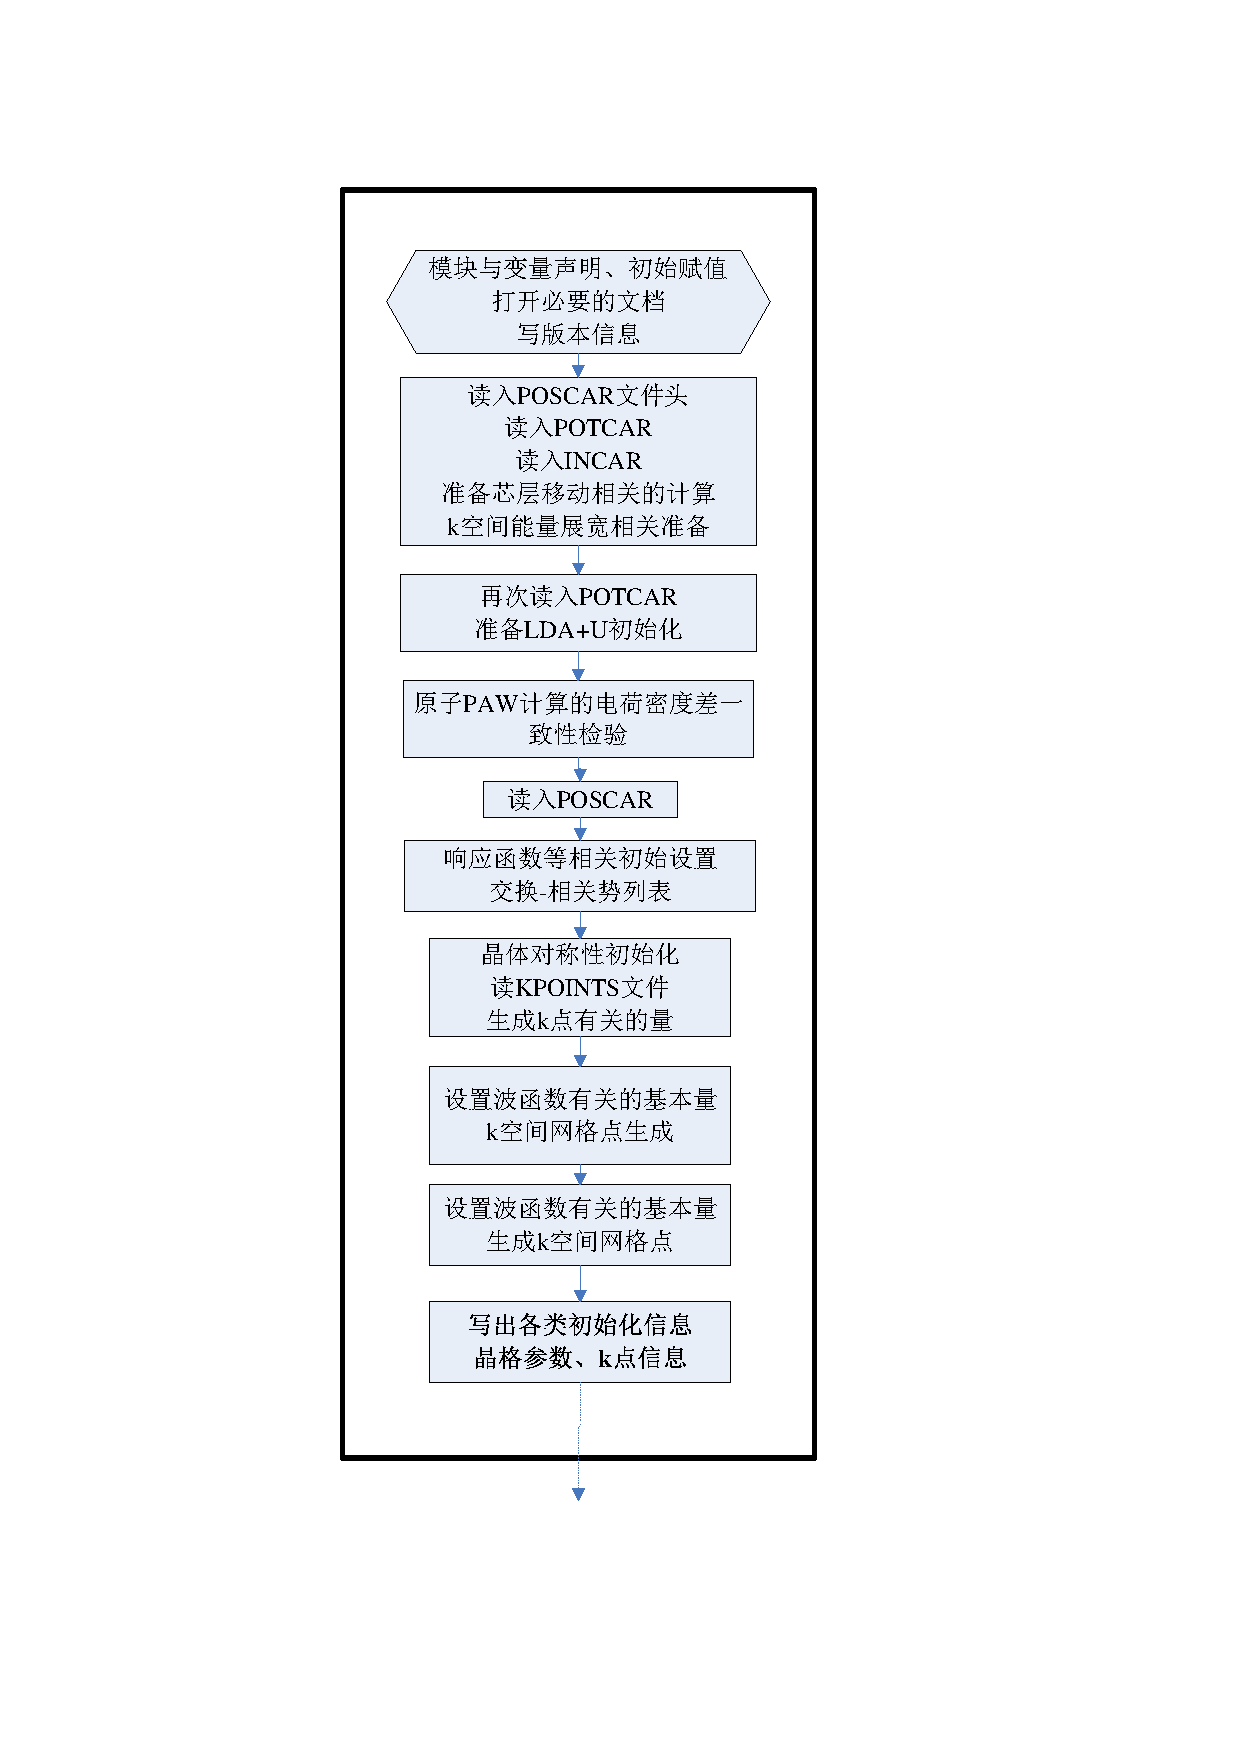
\includegraphics[height=3.62in,width=2.45in,viewport=160 118 395 755,clip]{Figures/VASP_main_Flow-1.pdf}
\caption{\small \textrm{Calculation of the K-S ground-states.}}%
\label{VASP_Follow}
\end{figure}
}

\frame
{
\frametitle{}
\begin{figure}[h!]
\centering
\vspace*{-0.65in}
%\hspace*{-10pt}
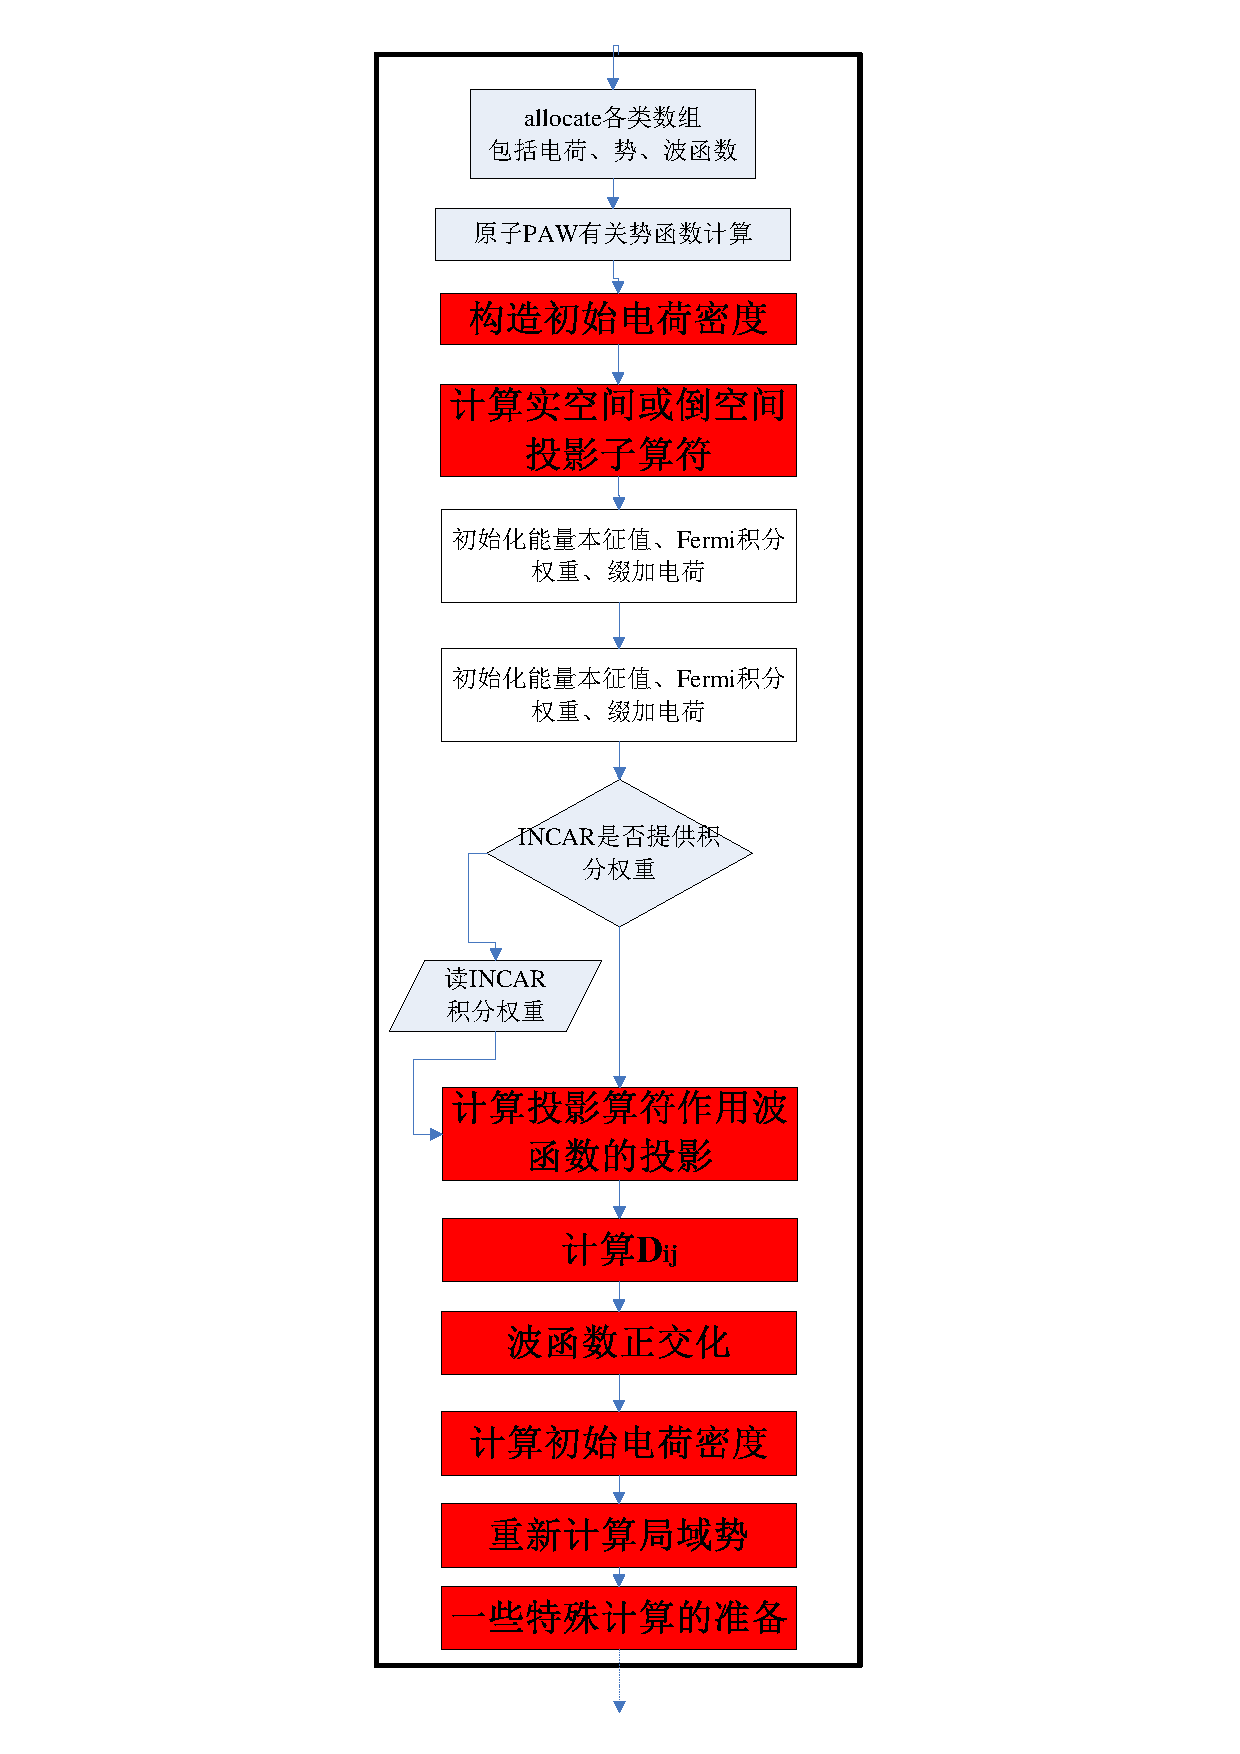
\includegraphics[height=3.62in,width=2.45in,viewport=176 16 416 819,clip]{Figures/VASP_main_Flow-2.pdf}
\caption{\small \textrm{Calculation of the K-S ground-states.}}%
\label{VASP_Follow}
\end{figure}
}

\frame
{
\frametitle{}
\begin{figure}[h!]
\centering
\vspace*{-0.65in}
%\hspace*{-10pt}
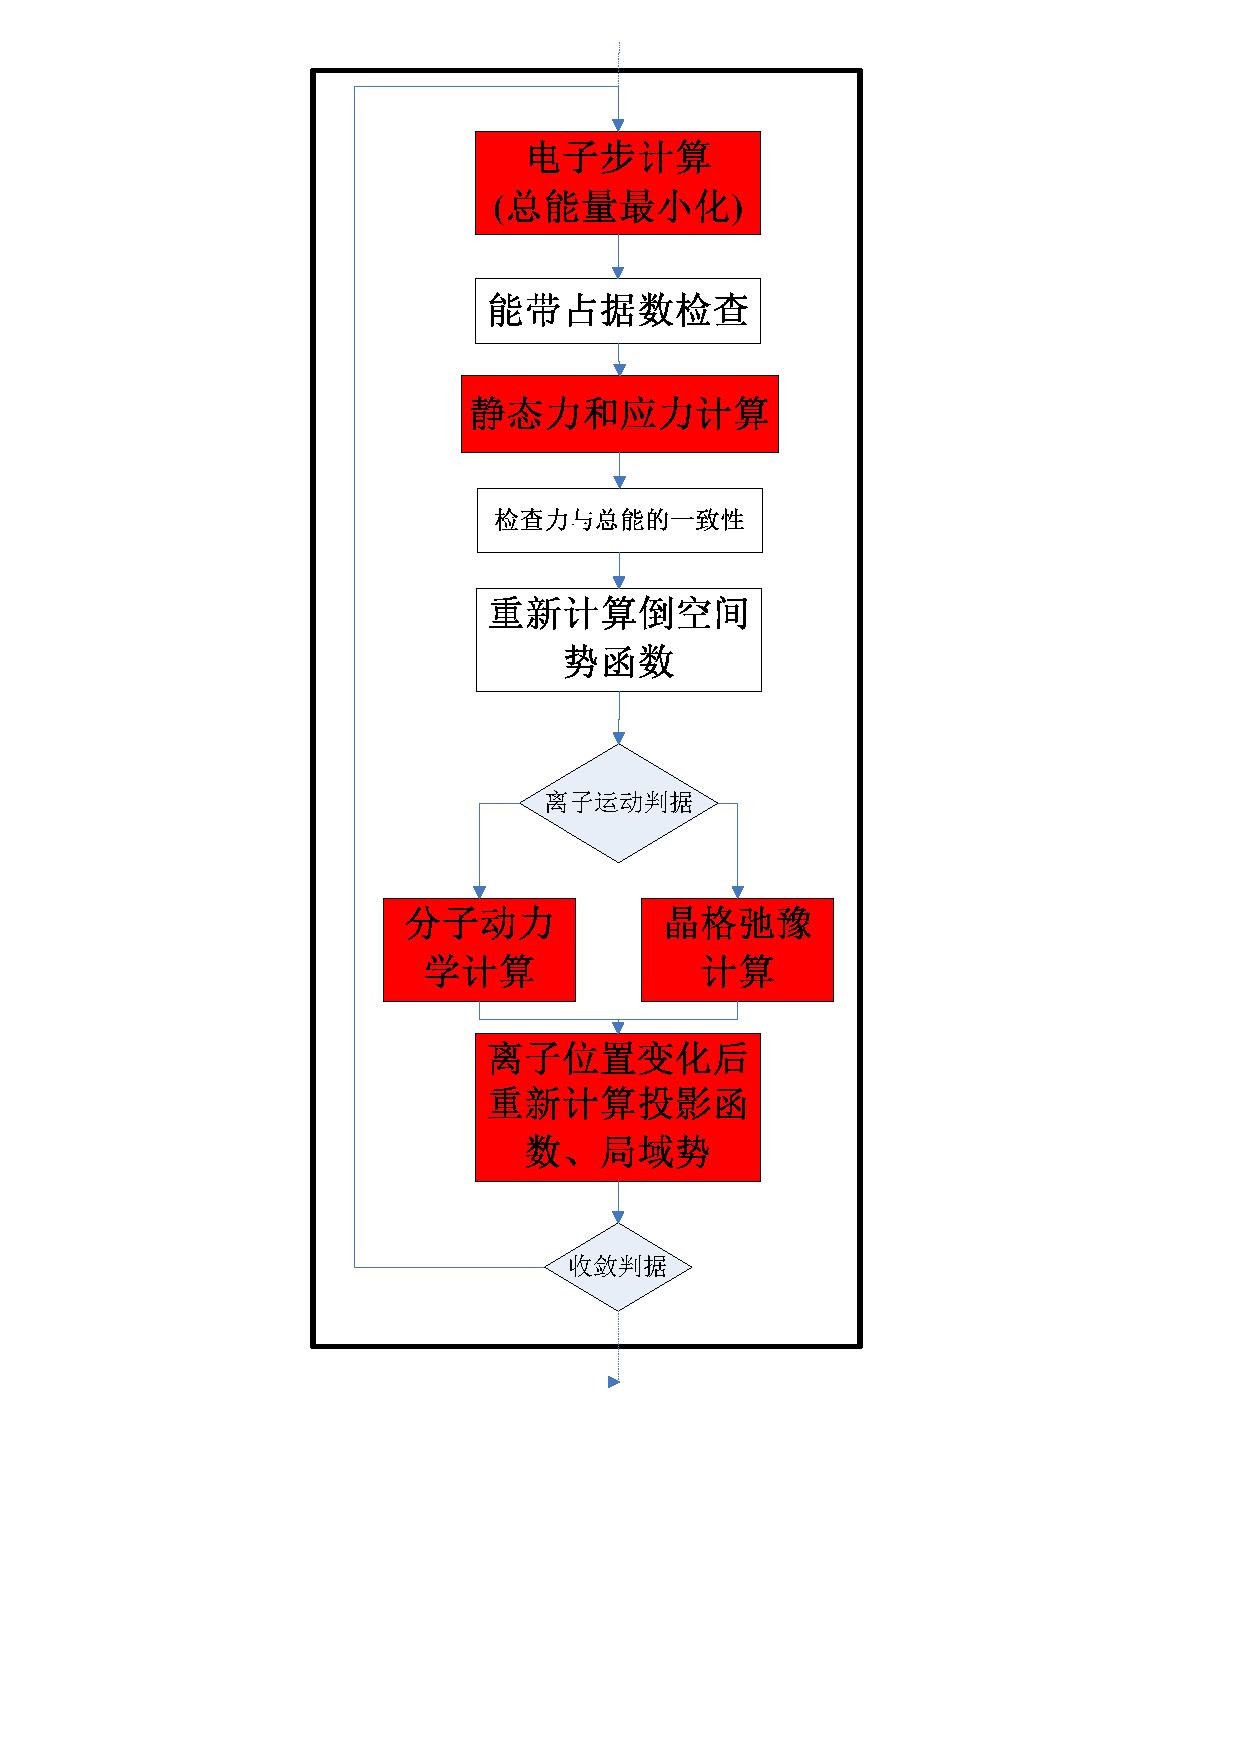
\includegraphics[height=3.62in,width=2.45in,viewport=146 173 416 812,clip]{Figures/VASP_main_Flow-3.pdf}
\caption{\small \textrm{Calculation of the K-S ground-states.}}%
\label{VASP_Follow}
\end{figure}
}

\frame
{
\frametitle{}
\begin{figure}[h!]
\centering
\vspace*{-0.65in}
%\hspace*{-10pt}
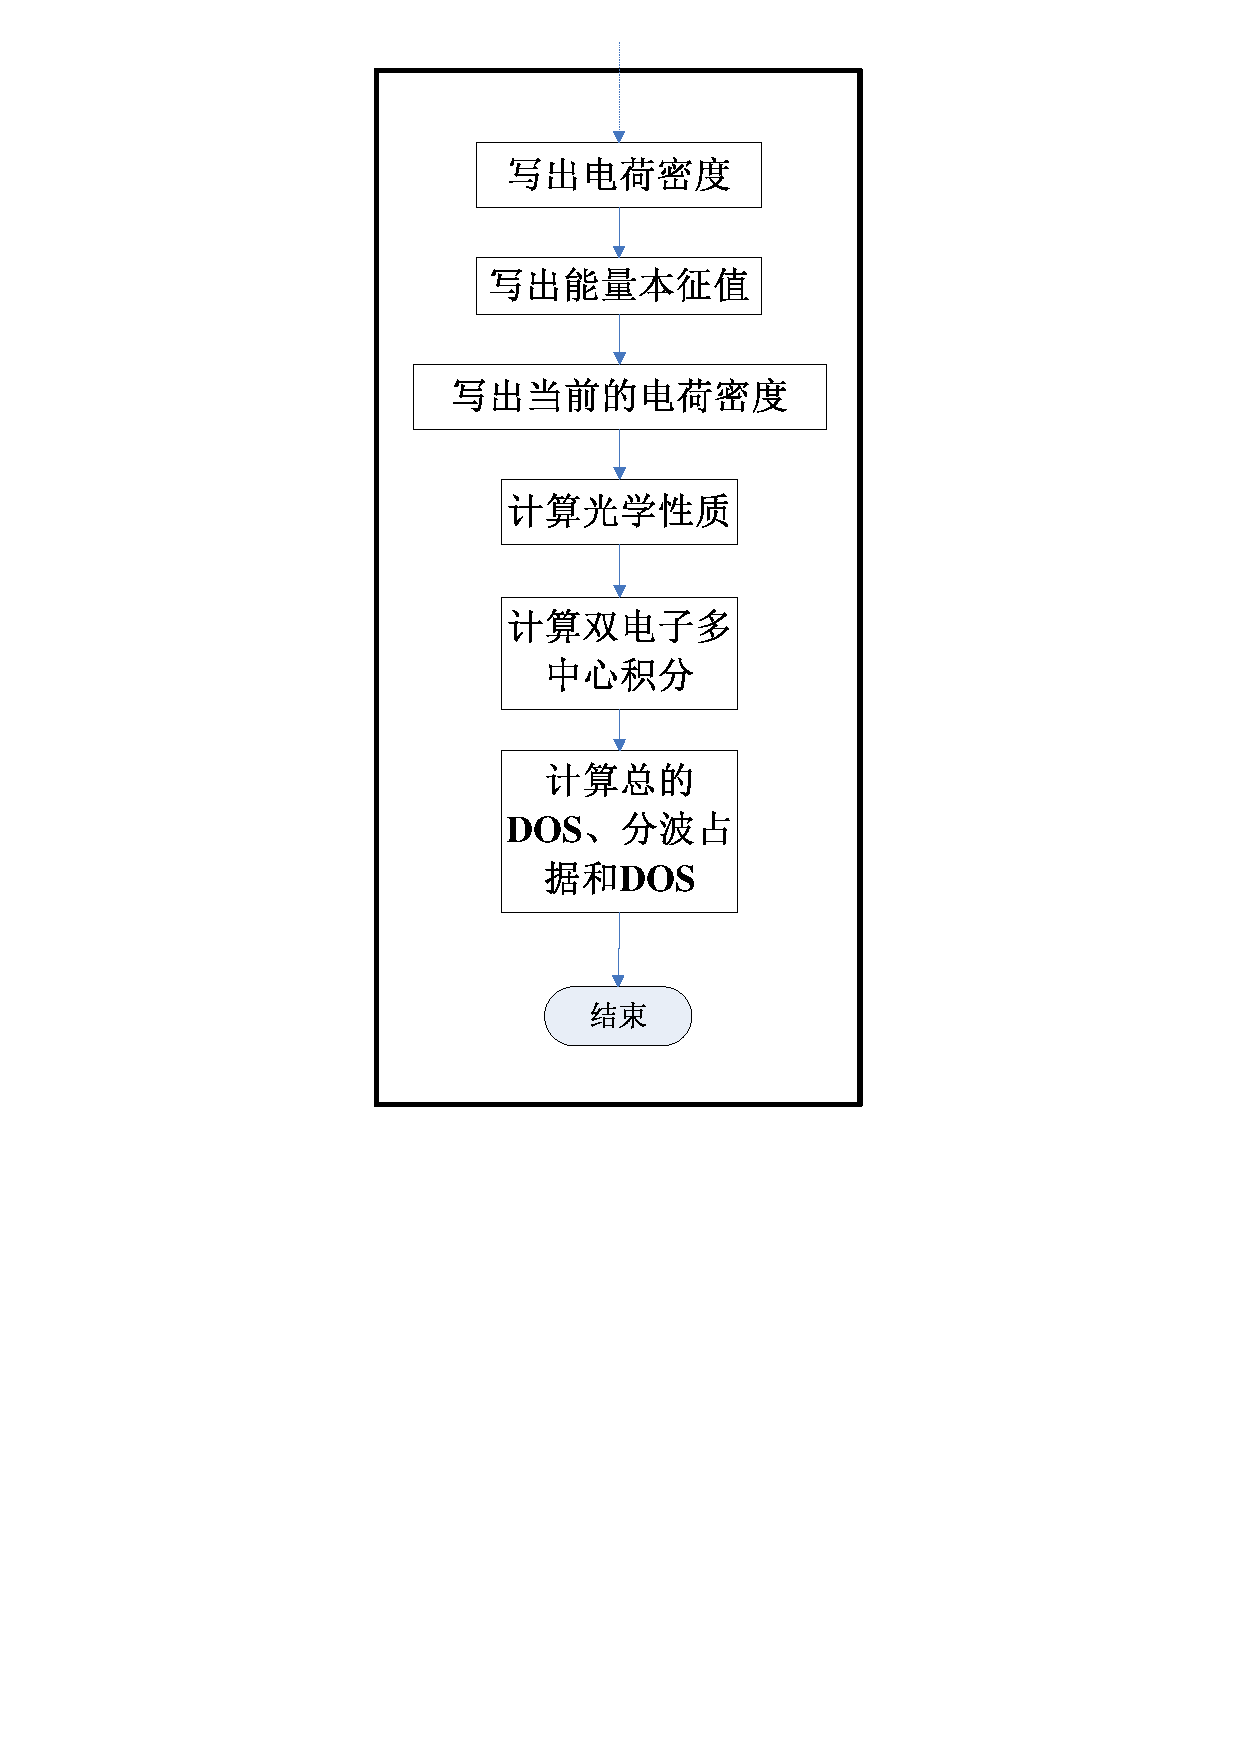
\includegraphics[height=3.62in,width=2.45in,viewport=177 305 417 813,clip]{Figures/VASP_main_Flow-4.pdf}
\caption{\small \textrm{Calculation of the K-S ground-states.}}%
\label{VASP_Follow}
\end{figure}
}

\section{能量密度方法}
\frame
{
	\frametitle{能量密度方法}
	\begin{itemize}
		\item 有关电子态问题的处理,$\vec k$-空间与电子的本征态对应,因此比较方便,但是一旦涉及材料的力学有关的物理量,则需要在正空间中考虑问题,能量密度方法是基于\textrm{DFT}最直接的方法
		\item \textcolor{red}{能量密度}的定义
	\begin{displaymath}
		E_{\mathrm{tot}}=\int_{\Omega_c}\textcolor{magenta}{\varepsilon_{\mathrm{tot}}(\vec r)}\mathrm{d}\vec r^3
	\end{displaymath}
		\item 	根据能量密度的定义,必须要回到传统能量计算的问题上\\
			一般地,在\textrm{DFT}理论中,能量密度可以表示为
	{\fontsize{9.0pt}{8.2pt}\selectfont{\begin{displaymath} 
		\varepsilon_{\mathrm{tot}}(\vec r)=\varepsilon_{\mathrm{kin}}(\vec r)+\varepsilon_{\mathrm{XC}}(\vec r)+\varepsilon_{\mathrm{H}}(\vec r)+\varepsilon_{\mathrm{local}}(\vec r)+\varepsilon_{\mathrm{ovrl-self}}(\vec r)+\varepsilon_{\mathrm{non-local}}(\vec r)
	\end{displaymath}}}
	\end{itemize}
}

\frame
{
	\frametitle{\textrm{PAW}框架下能量密度方法的表达}
	\begin{displaymath}
		\varepsilon_{\mathrm{kin}}(\vec r)=\bigg(\dfrac{\hbar^2}{2m}\bigg)\sum_{\vec R}\{\vec R|\vec t_{\vec R}\}\sum_n^{\mathrm{occ}}\sum_{\vec k\in\mathrm{I.P.}}f_{\vec kn}\omega_{\vec k}(\nabla\Psi_{\vec kn}(\vec r))^{\ast}\cdot(\nabla\Psi_{\vec kn}(\vec r))
	\end{displaymath}
	\begin{displaymath}
		\varepsilon_{\mathrm{XC}}(\vec r)=\epsilon(\vec r)n(\vec r)
	\end{displaymath}
	\begin{displaymath}
		\varepsilon_{\mathrm{H}}(\vec r)=n_{\mathrm{tot}}(\vec r)V_{\mathrm{H}}^{\mathrm{tot}}(\vec r)
	\end{displaymath}
	\begin{displaymath}
		\varepsilon_{\mathrm{local}}(\vec r)=n_{\mathrm{e}}(\vec r)V_{\mathrm{local}}^{\prime}(\vec r)
	\end{displaymath}
	{\fontsize{7.5pt}{7.2pt}\selectfont{\begin{displaymath}
		\varepsilon_{\mathrm{ovrl-self}}(\vec r)=\sum_{\vec t_a}\delta(\vec r-\vec t_a)\dfrac{e^2}2\bigg[\sum_{\vec R}\sideset{}{^{\prime}}\sum_{\vec ta^{\prime}}\dfrac{Z_aZ_{a^{\prime}}}{|\vec t_{a^{\prime}}+\vec R-\vec t_a|}\mathrm{erfc}\bigg(\dfrac{|\vec t_{a^{\prime}}+\vec R-\vec t_a|}{\sqrt2R_c}\bigg)-\sqrt{\dfrac{2}{\pi}}\dfrac{Z_a^2}{R_c}\bigg]
	\end{displaymath}}}
	{\fontsize{6.3pt}{6.2pt}\selectfont{\begin{displaymath}
		\varepsilon_{\mathrm{non-local}}(\vec r)=\sum_{\vec t_a}\delta(\vec r-\vec t_a)\bigg\{K_{ij}^a+V_{ij}^a+\sum_{kl}\dfrac{e^2}2\rho_{kl}^aW_{ij;kl}^a+\overline{E_{xc}[n_a^1+n_c^a]}-\overline{E_{xc}[\tilde n_z^1+\hat n_a^1+\tilde n_c^a]}\bigg\}
	\end{displaymath}}}

}
\appendix
%------------------------------------------------------------------------Reference----------------------------------------------------------------------------------------------
%\begin{thebibliography}{99}
%-----------------------------------------------------------------------------------------------------------------------------------------------------------------------%
%\frame
%{
%\frametitle{主要参考文献}
%{\small
%\bibitem{Singh_Book}\textrm{D. J. Singh. \textit{Plane Wave, PseudoPotential and the LAPW method} (Kluwer Academic, Boston,USA, 1994)}					%
%  \nocite{*}																				%
%}
%}
%\end{thebibliography}
\begin{thebibliography}{99}
\frame
{
\frametitle{主要参考文献}
{\small
	\bibitem{PR136-B864_1964}\textrm{P. Hohenberg and W. Kohn \textit{Phys. Rev.} \textbf{136} (1964), B864}
	\bibitem{PR140-A1133_1965}\textrm{W. Kohn and L.J. Sham \textit{Phys. Rev.} \textbf{140} (1965), A1133}
	\bibitem{PRL49-1691_1982}\textrm{P. Perdew, R. G. Parr, M. Levy and J. L. Balduz, Jr., \textit{Phys. Rev. Lett.} \textbf{49} (1982), 1691}
	\bibitem{Parr_Yang}\textrm{R.G. Parr and W. Yang. \textit{Density-Functional Theory of Atoms and Molecules} (Oxford University Press, New York, U.S.A., 1989)}
	\bibitem{Huang_Han}黄昆\:原著、韩汝琦\:改编, {\textit{固体物理学}}\:高等教育出版社, 北京, 1988
	\bibitem{Xie_Lu}谢希德、陆栋\:主编, {\textit{固体能带理论}}\:复旦大学出版社, 上海, 1998
	\bibitem{Xu_Li_Wang}徐光宪、黎乐民、王德民, {\textit{量子化学——基本原理和从头计算法}}\;\textrm{({\textit{上、中}})}\:科学出版社, 北京, 1980
}
}

\frame
{
\frametitle{主要参考文献}
{\small
	\bibitem{Elect_Stru}\textrm{Richard. M. Martin. \textit{Electronic Structure: Basic Theory and Practical Methods} (Cambridge University Press, Cambridge, England, 2004)}
	\bibitem{PR57-1169_1940}\textrm{C. Herring. \textit{Phys. Rev.}, \textbf{57} (1940), 1169}
	\bibitem{PR116_1959}\textrm{J. C. Phillips and L. Kleinman. \textit{Phys. Rev.} (1959), 116}
	\bibitem{PRL43-1494_1979}\textrm{D. R. Hamann, M. Schl\"uter and C. Chiang. \textit{Phys. Rev. Lett.} \textbf{43} (1979), 1494}
	\bibitem{Singh_Book}\textrm{D. J. Singh. \textit{Plane Wave, PseudoPotential and the LAPW method} (Kluwer Academic, Boston,USA, 1994)}
	\bibitem{PRB41-7892_1990}\textrm{D. Vanderbilt. \textit{Phys. Rev.} B, \textbf{41} (1990), 7892} 
	\bibitem{JPCM6-8245_1994}\textrm{G. Kresse and J. Hafner. J. Phys: \textit{Condens. Matter}, \textbf{6} (1994), 8245}
}
%{\small
%\phantomsection\addcontentsline{toc}{section}{Bibliography}	 %直接调用\addcontentsline命令可能导致超链指向不准确,一般需要在之前调用一次\phantomsection命令加以修正	%
%\bibliography{Myref}																			%
%\bibliographystyle{mybib}																		%
%  \nocite{*}																				%
%}
%-----------------------------------------------------------------------------------------------------------------------------------------------------------------------%
}

\frame
{
\frametitle{主要参考文献}
{\small
	\bibitem{PRB50-17953_1994}\textrm{P. E. Bl\"ochl. \textit{Phys. Rev.} B, \textbf{50} (1994), 17953}
	\bibitem{PRB59-1758_1999}\textrm{G. Kresse and D. Joubert \textit{Phys. Rev.} B, \textbf{59} (1999), 1758}
	\bibitem{VASP_UG}\textrm{G. Kresse, M. Marsman, and J. Furthm\"uller. \textit{VASP the GUIDE}. Computational Physics, Faculty of Physics, Universit\"at Wien, Austria (2012) \\\url{http://cms.mpi.univie.ac.at/VASP/}}
	\bibitem{Comp_Method}\textrm{V. V. Nemoshkalenko and V. N. Antonov. \textit{Computational Methods in Solid State Physics} (Gordon and Breach Science Publisher, Amsterdam, The Netherlands, 1998)}
        \bibitem{PRB47-10142_1993}\textrm{K. Laasonen, A. Pasquarello, R. Car, C. Lee and D. Vanderbilt \textit{Phys. Rev.} B, \textbf{47} (1993), 10142}
}
}

\frame
{
\frametitle{主要参考文献}
{\small
	\bibitem{PRB12-3060_1975}\textrm{O. K. Andersen. \textit{Phys. Rev.} B, \textbf{12} (1971), 3060}
	\bibitem{PR94-1111_1954}\textrm{W. Kohn and N. Rostocker. \textit{Phys. Rev.} \textbf{94} (1954), 1111}
	\bibitem{Andersen_Book}\textrm{O. K. Andersen. \textit{Computational Methods in Band Theory} (Plenum, New York, USA, 1971)}
	\bibitem{LMTO_Book}\textrm{H. Skriver. \textit{The LMTO method} (Springer, New York, USA, 1984)}
	\bibitem{Crelle30-51_1846}\textrm{C. G. Jacobi,\textbf{\"Uber ein leichtes Verfahren die in der Theorie der S\"acul\"arst\"orrungen vorkommenden Gleichungen numerisch aufzul\"osen}, \textit{Crelle's J.} \textbf{30} (1846), 51-94}
}
}

\frame
{
\frametitle{主要参考文献}
{\small
        \bibitem{CMS6-15_1996}\textrm{G. Kresse and J. Furthm\"uller \textit{Comput. Mat. Sci.}, \textbf{6} (1996), 15}
	\bibitem{PRB54-11169_1996}\textrm{G. Kresse and J. Furthm\"uller, \textit{Phys. Rev.} B, \textbf{54} (1996), 11169}
	\bibitem{JPC12-4409_1979}\textrm{J. Ihm, A. Zunger and L. Cohen, \textit{J. Phys.} C:, \textbf{12}, (1979), 4409}
	\bibitem{PRB45-6074_1992}\textrm{N. Chetty and R. M. Martin, \textit{Phys. Rev.} B, \textbf{45}, (1992), 6074}
}
\nocite*{}
}

%-----------------------------------------------------------Beamer下不建议使用bib,因为涉及分页--------------------------------------------------------------------------%
%{\small
%\phantomsection\addcontentsline{toc}{section}{Bibliography}	 %直接调用\addcontentsline命令可能导致超链指向不准确,一般需要在之前调用一次\phantomsection命令加以修正	%
%\bibliography{Myref}																			%
%\bibliographystyle{mybib}																		%
%  \nocite{*}																				%
%}

%------------------------------------------------------------------------------------------------------------------------------------------------------------------------------%

\end{thebibliography}
\section{附录1:~方程迭代求解与函数优化}
\frame
{
	\frametitle{非线性方程的\rm{Newton~}法求根}
	\textcolor{blue}{不管哪一种数值算法,其设计原理都是将复杂转化为简单的重复,或者说,通过简单的重复生成复杂}:\\\textcolor{red}{在算法设计和算法实现过程中,重复就是力量}
\begin{figure}[h!]
\centering
\animategraphics[autoplay, loop, height=2.1in]{1}{Figures/OP_Newton_}{0}{17}
\label{Equation_Newon}
\end{figure}
}

\frame
{
	\frametitle{迭代优化基本思想}
	对于给定函数$f$,在极值点,函数的梯度满足
	\begin{displaymath}
		\nabla f=0
	\end{displaymath}
	可将函数极值问题转化成方程求根问题
\begin{figure}[h!]
\centering
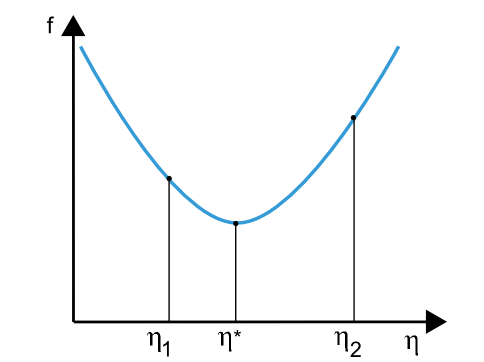
\includegraphics[height=1.68in,width=1.95in,viewport=30 0 450 360,clip]{Figures/OP_mini-1.png}
\hskip 0.1in
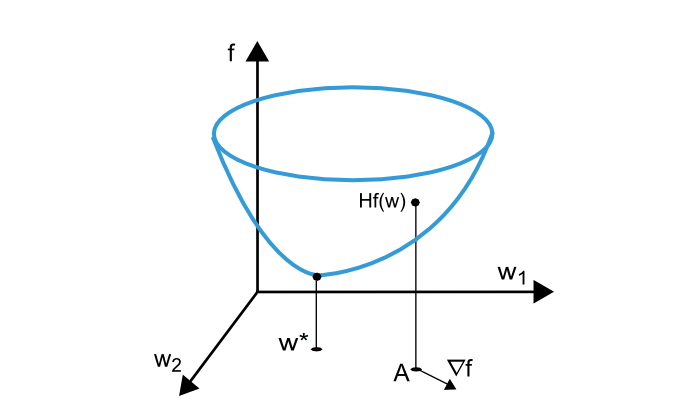
\includegraphics[height=1.68in,width=1.95in,viewport=150 20 560 390,clip]{Figures/OP_mini-2.png}
\label{OP_mini}
\end{figure}
}

\frame
{
	\frametitle{\textrm{Method of steepest descent}}
	对于函数$f(\mathbf{x}_0)$当前位置$\mathbf{x}_0$的负梯度方向$\mathbf{g}_0$满足
	\begin{displaymath}
		\mathbf{g}_0=-\nabla f(\mathbf{x}_0)
	\end{displaymath}
	用$\mathbf{g}_0$方向作为搜索方向,
	\begin{displaymath}
		\mathbf{x}=\mathbf{x}_0+\lambda\mathbf{g}_0,\qquad \lambda>0
	\end{displaymath}
	因为负的梯度方向为当前位置的最快下降方向,所以被称为“\textcolor{blue}{最陡下降法}”\\
	对函数$f$最小化参数$\lambda$,可确定下一步$\mathbf{x}_1$,可有
	\begin{displaymath}
		\dfrac{\mathrm{d}}{\mathrm{d}\lambda}f(\mathbf{x}_0+\lambda\mathbf{g})_0=\mathbf{g}_0\cdot\nabla f(\mathbf{x}_1)=\mathbf{g}_0\cdot\mathbf{g}_1=0
	\end{displaymath}
	因此\textcolor{red}{最速下降法最近邻两步的梯度彼此相互垂直}\\
	\textcolor{purple}{最陡下降法的收敛:~}\\靠近极小值时收敛速度减慢,越接近目标,步长越小,前进越慢
}

\frame
{
	\frametitle{\textrm{Conjugate gradient}}
	假设函数在接近极值附件,近似有二次函数的形式
	\begin{displaymath}
		f(\mathbf{x})=f_0+\frac12\mathbf{x}\cdot\mathbf{H}{\mathbf{x}}+\cdots
	\end{displaymath}
	其中$\mathbf{H}$是\textcolor{blue}{\textrm{Hessian}矩阵},定义为
	\begin{displaymath}
		H_{ij}=\dfrac{\partial^2f(\mathbf{x})}{\partial x_i\partial x_j}
	\end{displaymath}
	当$f$的偏导连续,则$\mathbf{H}$是对称矩阵,并且一般要求$\mathbf{H}$是正定的
	\vskip 20pt
	设从点$\mathbf{x}_i$出发沿方向$\mathbf{h}_i$(\textcolor{blue}{不再限于梯度$\mathbf{g}_i$方向}),前进到点$\mathbf{x}_{i+1}$,由根据最小化要求
	\begin{displaymath}
		\mathbf{h}_i\cdot\nabla f(\mathbf{x}_{i+1})=0
	\end{displaymath}
	为确定$\mathbf{x_{i+1}}$点的继续前进方向$\mathbf{h}_{i+1}$,设$\mathbf{x}_{i+1}$可由$\mathbf{x}_i+\lambda\mathbf{h}_{i+1}$得到,因此$\mathbf{x}_{i+1}$的梯度
	\begin{displaymath}
		\mathbf{g}_{i+1}=\nabla f(\mathbf{x}_{i+1})=-\mathbf{H}\mathbf{x}_{i+1}=-\mathbf{H}(\mathbf{x}_{i}+\lambda\mathbf{h}_{i+1})
	\end{displaymath}
}

\frame
{
	\frametitle{\textrm{Conjugate gradient}}
	与方向$\mathbf{h}_i$相比,梯度的改变为
	\begin{displaymath}
		\Delta\mathbf{g}=-\lambda\mathbf{H}\mathbf{h}_{i+1}
	\end{displaymath}

	根据最小化要求,梯度的改变与$\mathbf{h}_i$方向正交
	\begin{displaymath}
		\mathbf{h}_i\cdot\mathbf{H}\mathbf{h}_{i+1}=0
	\end{displaymath}
	共轭梯度法算法:对于给定函数
	\begin{itemize}
		\item 已知初值$\mathbf{x}_0$和梯度$\mathbf{g}_0$,取初始方向$\mathbf{h_0}=\mathbf{g}_0$(\textcolor{blue}{最陡下降})
		\item 根据递推关系确定
			\begin{displaymath}
				\begin{aligned}
					\mathbf{g}_{i_+1}=&\mathbf{g}_{i_+1}-\lambda_i\mathbf{H}\mathbf{h}_{i}\qquad \lambda_i=\dfrac{\mathbf{g}_i\cdot\mathbf{g}_i}{\mathbf{g}_i\cdot\mathbf{H}\mathbf{h}_i}\\	
					\mathbf{h}_{i_+1}=&\mathbf{g}_{i_+1}+\gamma_i\mathbf{h}_{i}\qquad \gamma_i=-\dfrac{\mathbf{g}_{i+1}\cdot\mathbf{H}\mathbf{h}_i}{\mathbf{h}_i\cdot\mathbf{H}\mathbf{h}_i}\\	
					\mathbf{x}_{i_+1}=&\mathbf{x}_{i}+\lambda_i\mathbf{h}_{i}
				\end{aligned}
			\end{displaymath}
	\end{itemize}
	\textcolor{purple}{共轭梯度法:~步收敛性,稳定性高,不需要任何外来参数}
}

\frame
{
	\frametitle{最陡下降与共轭梯度}
\begin{figure}[h!]
\centering
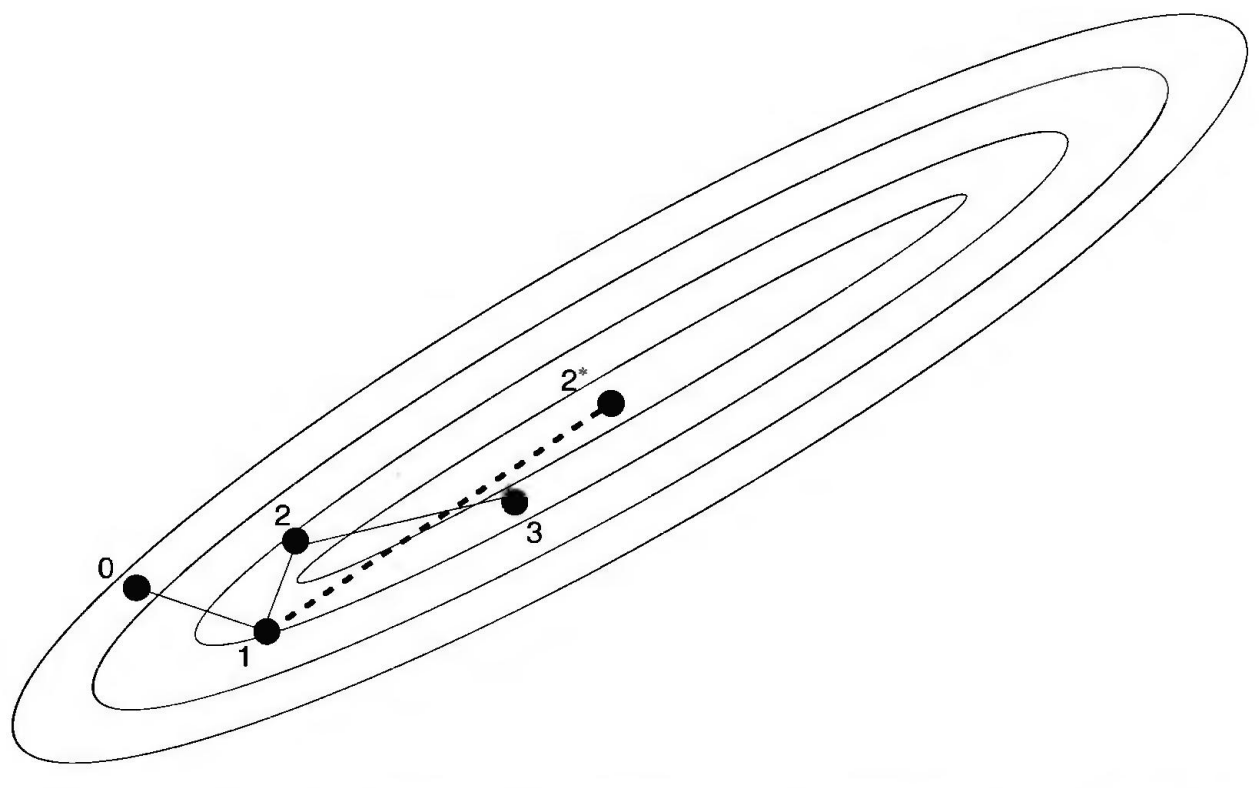
\includegraphics[height=2.0in,width=3.5in,viewport=0 0 950 590,clip]{Figures/OP_descent_CG.png}
\label{decent_CG}
\caption{\small \textrm{Schematic illustration of minimization of a function in two dimensions. The steps 1,2,3,$\cdots$ denote the steepest descent steps and the point $2^{\ast}$ denote the conjugate gradient path that reaches the exact solution after two steps if the functional is quadratic.}}%(与文献\cite{EPJB33-47_2003}图1对比)
\end{figure}
}

\frame
{
	\frametitle{\textrm{Quasi-Newton Methods}}
	求解方程
	\begin{displaymath}
		f(\mathbf{x})=\mathbf{x}
	\end{displaymath}
	$\mathbf{x}$是函数$f(\mathbf{x})$的\textcolor{red}{不动点}
	
	对这类问题的求解,可以利用迭代关系
	\begin{displaymath}
		\mathbf{x}_{i+1}=f(\mathbf{x}_i)\qquad (i=1,2,3,\cdots)
	\end{displaymath}
	这称为\textcolor{blue}{不动点迭代法}

	另一种求解策略是定义残量
	\begin{displaymath}
		R[\mathbf{x}]=f(\mathbf{x})-\mathbf{x}
	\end{displaymath}
	最小化残量的模$|R[\mathbf{x}]|$,特别是当残量$R[\mathbf{x}]$近似是$\mathbf{x}$的线性函数,可有\textcolor{purple}{Jacobian}矩阵
	\begin{displaymath}
		\mathbf{J}=\dfrac{\delta R[\mathbf{x}]}{\delta\mathbf{x}}
	\end{displaymath}
	可通过迭代关系求解原方程的解
	\begin{displaymath}
		\mathbf{x}_{i+1}=\mathbf{x}_{i}-\mathbf{J}^{-1}R[\mathbf{x}_{i}]
	\end{displaymath}
}

\section{附录2:~矩阵直接对角化与迭代对角化}
%\subsubsection{矩阵直接对角化算法}
\frame
{
	\frametitle{相似矩阵}
\textcolor{blue}{相似矩阵}:~设$\mathbf{A}$,$\mathbf{B}$都是\textrm{n}阶矩阵,若有可逆矩阵$\mathbf{P}$,使得
	\begin{displaymath}
		\mathbf{P}^{-1}\mathbf{A}\mathbf{P}=\mathbf{B}
	\end{displaymath}
	则称$\mathbf{B}$是$\mathbf{A}$的相似矩阵,或说$\mathbf{A}$和$\mathbf{B}$相似
	\begin{itemize}
		\item 相似矩阵具有\textcolor{red}{相同的}\textcolor{blue}{本征向量}和\textcolor{blue}{本征值}
		\item 若$\mathbf{A}$相似于\textcolor{brown}{对角矩阵}$\boldsymbol{\Lambda}$,则$\boldsymbol{\Lambda}$主对线上元素是$\mathbf{A}$的\textrm{n}个本征值
		\item \textrm{n}阶方阵$\mathbf{A}$能与对角矩阵$\boldsymbol{\Lambda}$相似的充分必要条件:~$\mathbf{A}$有\textrm{n}个\textcolor{magenta}{线性无关}的本征向量
		\item 实对称矩阵的特征值为实数
		\item \textcolor{purple}{实对称矩阵不同的本征值所对应的本征向量线性无关}
	\end{itemize}
}

\frame
{
	\frametitle{\textrm{QR}分解与矩阵的对角化}
	\textrm{QR~}方法本质上是一种变换方法,是计算一般矩阵(中小型矩阵)的全部本征值的最有效方法之一
\vskip 5pt
	所谓\textrm{QR}分解,就是将一个矩阵(以实对称方针为例)分解成一个\textcolor{blue}{正交矩阵}和一个\textcolor{blue}{上三角矩阵}。即
	\begin{displaymath}
		\mathbf{A}=\mathbf{Q}\mathbf{R}
	\end{displaymath}
	其中$\mathbf{Q}$是正交矩阵,即$\mathbf{Q}$中的列向量互相正交,即
	\begin{displaymath}
		\mathbf{Q}^{-1}\mathbf{Q}=\mathbf{I} 
	\end{displaymath}
	$\mathbf{R}$是上三角矩阵,可得到新矩阵$\mathbf{B}$
	\begin{displaymath}
		\mathbf{B}=\mathbf{R}\mathbf{Q}=\mathbf{Q}^{-1}\mathbf{A}\mathbf{Q}
	\end{displaymath}
	$\mathbf{B}$与$\mathbf{A}$是相似矩阵,可以再对$\mathbf{B}$进行\textrm{QR~}分解\\
	\textcolor{red}{当$\mathbf{A}$为非奇异矩阵时,这个分解是唯一的}
	\begin{itemize}
		\item 实现\textrm{QR}分解的算法有多种,包括\textrm{Gram–Schmidt~}正交化,\textrm{Householder~}变换,以及\textrm{Givens~}旋转等
	\end{itemize}
}

\frame
{
	\frametitle{矩阵的迭代对角化}
	\begin{itemize}
		\item 矩阵的直接对角化计算量 $O(N^3)$
		\item 矩阵的迭代对角化 $O(N_0^2\times N\ln N)\quad N_0\ll N$
	\end{itemize}
	\textcolor{blue}{迭代求本征值的思想是\textrm{Jacobian~}于\textrm{1846~}年提出的}\upcite{Crelle30-51_1846}\\
	其基本思想是
	\begin{displaymath}
		(H-\varepsilon^n)|\psi^n\rangle=|R[\psi^n]\rangle
	\end{displaymath}
	这里$n$是迭代步数,$|\psi^n\rangle$和$\varepsilon^n$分别是本征态和本征值,$|R[\psi^n]\rangle$是残矢量
	\vskip 10pt
	在电子态计算过程中,选择适当的基函数,可以使\textrm{Schr\"odinger~}方程的矩阵接近对角阵,因此可有
	\begin{displaymath}
		|\psi\rangle=\mathbf{D}^{-1}(\mathbf{H}-\varepsilon)|\psi\rangle+|\psi\rangle
	\end{displaymath}
	这里$\mathbf{D}$是非奇异矩阵,与$\mathbf{H}$矩阵有关,可根据需要选取多种形式
}

\frame
{
	\frametitle{稀疏矩阵的\textrm{Lanczos~}算法}
	对于稀疏矩阵$\mathbf{A}$,取任意矢量$\psi_0$(要求归一),构造矢量$\psi_1$(同样要求归一,并与$\psi_0$正交),满足
	\begin{displaymath}
		\mathbf{A}\psi_0=a_0\psi_0+b_0\psi_1
	\end{displaymath}
	由此确定$a_0$、$b_0$、$\psi_1$
	\begin{displaymath}
		\begin{aligned}
			a_0&=\langle\psi_0|\mathbf{A}|\psi_0\rangle\\
			b_0\psi_1&=\mathbf{A}\psi_0-a_0\psi_0\\
			||\psi_1||&=1
		\end{aligned}
	\end{displaymath}
	进而可构造$\psi_2$:
	\begin{displaymath}
		\mathbf{A}\psi_1=c_1\psi_0+a_1\psi_1+b_1\psi_2
	\end{displaymath}
	要求$\psi_2$与$\psi_0$、$\psi_1$正交归一条件,确定$\psi_2$,$a_1$,$b_1$,$c_1$
}

\frame
{
	\frametitle{稀疏矩阵的\textrm{Lanczos~}算法}
	根据递推关系有
	\begin{displaymath}
		\mathbf{A}\psi_p=\sum_{q=0}^{p-1}c_p^{(q)}\psi_q+a_q\psi_p+b_p\psi_{p+1}
	\end{displaymath}
	这里$\psi_{p+1}$将与所有之前的$\psi_q$(\textrm{processors})正交

	利用矩阵$\mathrm{A}$的\textrm{Hermitian},因此可有等式
	\begin{displaymath}
		c_p^{(q)}=\langle\psi_q|\mathbf{A}\psi_p\rangle=\langle\mathbf{A}\psi_q|\psi_p\rangle=0
	\end{displaymath}
	即矢量$\psi_p$垂直于矢量$\mathbf{A}\psi_q$,由此可得
	\begin{displaymath}
		c_p^{(p-1)}=\langle\psi_{p-1}|\mathbf{A}\psi_p\rangle=\langle\mathbf{A}\psi_{p-1}|\psi_p\rangle=b_{p-1}
	\end{displaymath}
	经过$p$步迭代后
	\begin{displaymath}
		\mathbf{A}\psi_p=b_{p-1}\psi_{p-1}+a_p\psi_p+b_p\psi_{p+1}
	\end{displaymath}
	这里$\psi_{p+1}$要求与$\psi_p$和$\psi_{p-1}$满足正交归一条件
}

\section{附录3:~超软赝势的总能量表示}
\frame
{
	\frametitle{\textrm{US-PP}的总能量表示}
	根据\textrm{D. Vanderbilt}的超软赝势(\textrm{US-PP})方案
	原子波函数满足$$(T+V_{\mathrm{AE}}-\varepsilon_n)|\psi_n\rangle=0$$
	据此构造原子赝波函数$\phi_n$,在截断半径$r_c^l$处,$\phi_n$与$\psi_n$平滑衔接(不需要模守恒条件)

	类似地,构造局域平滑势$V_{loc}(r)$,在截断半径$r_c^{loc}$处,$V_{loc}(r)$与$V_{\mathrm{AE}}(r)$平滑衔接
	
	构造辅助轨道
	$$|\chi_n\rangle=(\varepsilon_n-T-V_{loc})|\phi_n\rangle$$
	由此构造内积矩阵,矩阵元$$B_{nm}=\langle\phi_n|\chi_m\rangle$$
	并有$$|\beta_n\rangle=\sum_m(B^{-1})_{mn}|\chi_m\rangle$$
	这里$\beta_n$是局域函数,并与$\phi_n$垂直
}

\frame
{
	\frametitle{\textrm{US-PP}的总能量表示}
	定义\textcolor{orange}{缀加函数}$$Q_{nm}(\vec r)=\psi_n^{\ast}(\vec r)\psi_m(\vec r)-\phi_n^{\ast}(\vec r)\phi_m(\vec r)$$
	\textcolor{blue}{可赝化的补偿电荷}$$q_{nm}=\langle\psi_n|\psi_m\rangle_R-\langle\phi_n|\phi_m\rangle_R$$
	由此可以导出$\phi_n$满足久期方程
	\begin{displaymath}
		\begin{aligned}
			&\left(T+V_{loc}+\sum_{nm}D_{nm}|\beta_n\rangle\langle\beta_m|\right)|\phi_n\rangle\\
			=&\varepsilon_n\left(1+\sum_{nm}q_{nm}|\beta_n\rangle\langle\beta_m|\right)|\phi_n\rangle
		\end{aligned}
	\end{displaymath}
	其中$$D_{nm}=B_{nm}+\varepsilon q_{nm}$$
}

\frame
{
	\frametitle{\textrm{US-PP}的总能量表示}
	在超软赝势方法中,包含$N_v$个价电子体系的总能量\upcite{PRB47-10142_1993}
	\begin{displaymath}
		\begin{aligned}
			E_{\mathrm{tot}}[\{\phi_i\},\{\vec R_I\}]=&\sum_i\langle\phi_i|-\frac12\nabla^2+V_{\mathrm{NL}}|\phi_i\rangle\\
			&+\frac12\iint\mathrm{d}\vec r\mathrm{d}\vec r\,^{\prime}\dfrac{n(\vec r)n(\vec r\,^{\prime})}{|\vec r-\vec r\,^{\prime}|}\\
			&+\int\mathrm{d}\vec r V_{loc}^{\mathrm{ion}}(\vec r)n(\vec r)+E_{\mathrm{XC}}[n]\\
			&+U(\{\vec R_I\})
		\end{aligned}
	\end{displaymath}
	这里$\phi$是体系波函数,$n(\vec r)$是电子密度,$E_{\mathrm{XC}}$是交换-相关能,$U(\{\vec R_I\})$是离子-离子相互作用能
}

\frame
{
	\frametitle{\textrm{US-PP}的总能量表示}
	电荷密度$$n(\vec r)=\sum_i\big[|\phi_i(\vec r)|^2+\sum_{nm,I}Q_{nm}^I(\vec r)\langle\phi_i|\beta_n^I\rangle\langle\beta_m^I|\phi_i\rangle\big]$$
	局域势$$V_{loc}^{\mathrm{ion}}(\vec r)=\sum_IV_{loc}^{\mathrm{ion}}(\vec r-\vec R_I)$$
	$V_{loc}^{\mathrm{ion}}$由$V_{loc}$去屏蔽后得到$$V_{loc}^{\mathrm{ion}}(r)=V_{loc}(r)-\int\mathrm{d}\vec r\,^{\prime}\dfrac{n(\vec r\,^{\prime})}{|\vec r-\vec r\,^{\prime}|}-\mu_{\mathrm{XC}}(r)$$
	非局域部分$$V_{\mathrm{NL}}=\sum_{nm,I}D_{nm}^{(0)}|\beta_n^I\rangle\langle\beta_m^I|$$
	这里$$D_{nm}^{(0)}=D_{nm}-\int\mathrm{d}\vec r\,^{\prime}V_{loc}(\vec r\,^{\prime})n(\vec r\,^{\prime})$$
}

\section{附录4:~赝势\rm{Data set}的生成}
\frame
{
	\frametitle{模守恒赝势构造流程}
\begin{figure}[h!]
\centering
%\vspace*{-0.10in}
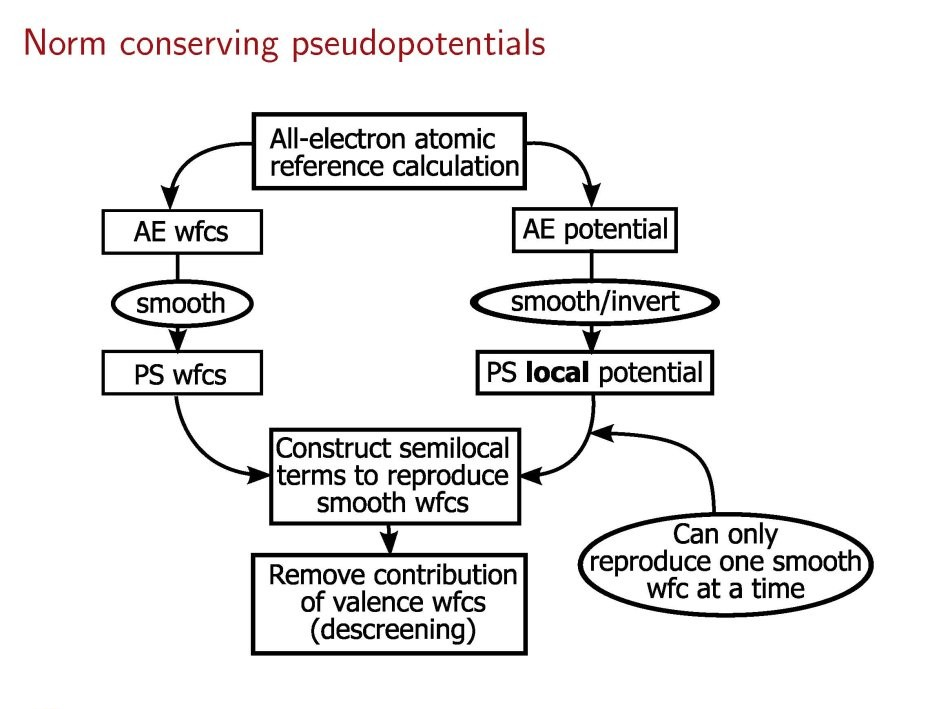
\includegraphics[height=2.70in,width=3.77in,viewport=70 40 900 610,clip]{Figures/Pseudo-NC.jpg}
%\caption{\small \textrm{Pseudopotential for metallic sodium, based on the empty core model and screened by the Thomas-Fermi dielectric function.}}%(与文献\cite{EPJB33-47_2003}图1对比)
\label{Pseudo-NC}
\end{figure}
}

\frame
{
	\frametitle{\textrm{PAW}原子数据集}
\textrm{PAW}原子数据集是在原子核附近$r_c$范围内将波函数用原子分波展开所需信息的统称,是\textrm{PAW}计算的基础。

\textrm{PAW}原子数据集主要包括
	\begin{itemize}
		\item 分波信息:原子分波$\phi_i$、赝分波$\tilde\phi_i$和投影子波函数$p_i$
		\item 密度信息:$r_c$内的电荷密度$n^1$、赝电荷密度$\tilde n^1$和补充电荷$\hat n$
		\item 赝势信息:局域赝势$\tilde v_{loc}(\vec r)$
	\end{itemize}
	与赝势方法相似,一套原子数据集将用于各种化学环境下的\textrm{PAW}计算,即要求原子数据集有良好的可移植性;与赝势方法不同之处在于\textrm{PAW}原子集中除了赝原子的信息,还包含了真实原子的信息。
}

\frame
{
	\frametitle{\textrm{PAW}原子数据集}
	原子分波:$$\bigg(-\dfrac12\nabla^2+v_{at}-\varepsilon_i^1\bigg)|\phi_i\rangle=0$$
	赝原子分波:$$\bigg(-\dfrac12\nabla^2+w_i(r)-\varepsilon_i^1\bigg)|\tilde\phi_i\rangle=0$$
	局域赝势:%$$w_i(r)=\tilde v_{at}(r)+c_ik(r)=\tilde v_{at}(0)\mathrm{e}^{-(r/r_k)^{\lambda}}+[1-k(r)]v_{at}(r)+c_i\mathrm{e}^{-(r/r_k)^{\lambda}}$$
	$$w_i(r)=\tilde v_{at}(0)\mathrm{e}^{-(r/r_k)^{\lambda}}+[1-\mathrm{e}^{-(r/r_k)^{\lambda}}]v_{at}(r)+c_i\mathrm{e}^{-(r/r_k)^{\lambda}}$$
\begin{figure}[h!]
\centering
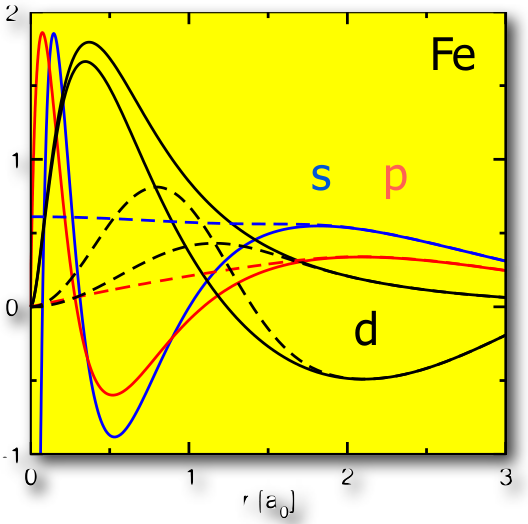
\includegraphics[height=1.2in,width=1.5in,viewport=0 0 570 545,clip]{Figures/PAW-partical.png}
\caption{\small \textrm{The partical-wave of Fe atom.}}%(与文献\cite{EPJB33-47_2003}图1对比)
\label{PAW_partical_Fe}
\end{figure}
}

\frame
{
	\frametitle{\textrm{PAW projector}}
	投影函数:$$|\tilde p_i\rangle=\bigg(-\dfrac12\nabla^2+\tilde v_{at}-\varepsilon_i^1\bigg)|\tilde\phi_i\rangle$$
	\textrm{Gram-Schmidt}正交化
	$$|\tilde p_i\rangle=|\tilde p_i\rangle-\sum_{j=1}^{i-1}|\tilde p_j\rangle\langle\tilde\phi_j|\tilde p_i\rangle$$
%	$$|\phi_i\rangle=|\phi_i\rangle-\sum_{j=1}^{i-1}|\phi_j\rangle\langle\tilde p_j|\tilde\phi_i\rangle$$
%	$$|\tilde\phi_i\rangle=|\tilde\phi_i\rangle-\sum_{j=1}^{i-1}|\tilde\phi_j\rangle\langle\tilde p_j|\tilde\phi_i\rangle$$
	$|\phi_i\rangle=|\phi_i\rangle-\sum\limits_{j=1}^{i-1}|\phi_j\rangle\langle\tilde p_j|\tilde\phi_i\rangle\quad|\tilde\phi_i\rangle=|\tilde\phi_i\rangle-\sum\limits_{j=1}^{i-1}|\tilde\phi_j\rangle\langle\tilde p_j|\tilde\phi_i\rangle$
\begin{figure}[h!]
\centering
\vspace*{-0.4in}
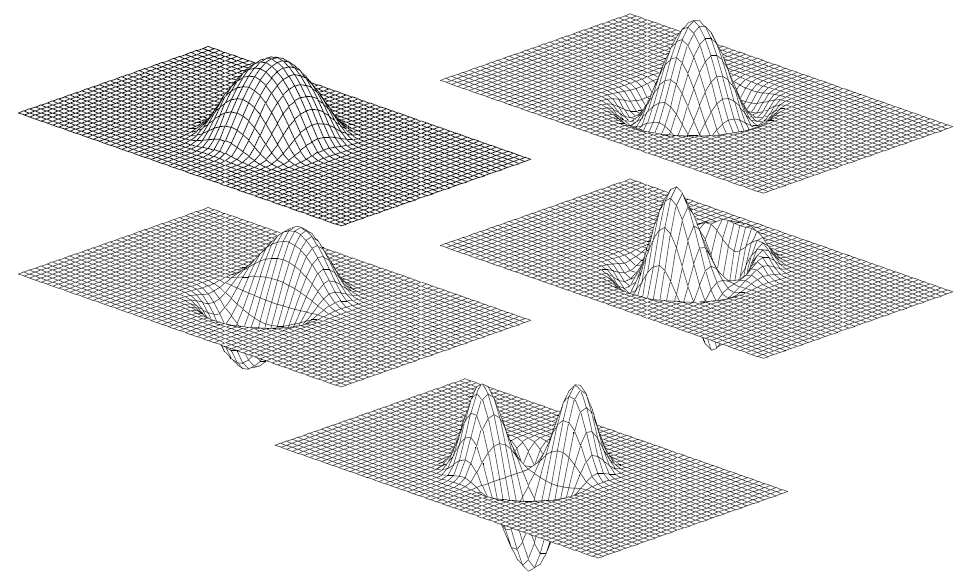
\includegraphics[height=1.5in,width=2.3in,viewport=0 0 1100 745,clip]{Figures/PAW_projector-2.png}
\caption{\small \textrm{The projector of PAW.}}%(与文献\cite{EPJB33-47_2003}图1对比)
\label{PAW_projector}
\end{figure}
\begin{itemize}
	\item 与分波具有相同的角动量$l$
	\item 局域在缀加区域(Augmentation region)
	\item 节点依次增加
\end{itemize}
}

\frame
{
	\frametitle{\textrm{局域势$\bar v$}}
	去屏蔽局域势:$$\bar v(r)=\tilde v_{at}(r)-\int\mathrm{d}r^{\prime}\dfrac{\tilde n(r^{\prime})+\hat n(r^{\prime})}{|r-r^{\prime}|}-\mu_{xc}[\tilde n(r)]$$
	其中$\tilde v_{at}(r)$的确定
	$$\bigg[-\dfrac12\nabla^2+\tilde v_{at}-\varepsilon+\sum_{(i,j)}|\tilde p_i\rangle\big(\mathrm{d}H_{ij}-\varepsilon\mathrm{d}O_{ij}\big)\langle\tilde p_j|\bigg]|\tilde\Psi_j\rangle=0$$
	其中$\mathrm{d}H_{ij}$和$\mathrm{d}O_{ij}$分别是
	$$\mathrm{d}H_{ij}=\langle\phi_i|-\dfrac12\nabla^2+v_{at}|\phi_j\rangle-\langle\tilde\phi_i|-\dfrac12\nabla^2+\tilde v_{at}|\tilde\phi_j\rangle$$
	$$\mathrm{d}O_{ij}=\langle\phi_i|\phi_j\rangle-\langle\tilde\phi_i|\tilde\phi_j\rangle$$
}

\frame
{
	\frametitle{\textrm{局域势$\bar v$}}
	如果解$$|\tilde\Psi\rangle=|u\rangle+\sum_i|w_i\rangle c_i$$
	其中$|u\rangle$和$|w_i\rangle$的定义分别为
	$$\big(-\frac12\nabla^2+\tilde v-\varepsilon\big)|u\rangle=0$$
	$$\big(-\frac12\nabla^2+\tilde v-\varepsilon\big)|w_i\rangle=|\tilde p_i\rangle$$
	因此可以得到
	$$c_i=-\sum_{j,l}\bigg[\delta_{ij}+\sum_k\mathrm{d}H_{ik}-\varepsilon\mathrm{d}O_{ik}\langle\tilde p_k|w_j\rangle\bigg]^{-1}\big(\mathrm{d}H_{jl}-\varepsilon\mathrm{d}O_{jl}\big)\langle p_l|u\rangle$$
}

%\frame
%{
%	\frametitle{\textrm{AtomPAW}程序包简介}
%	\textrm{AtomPAW}程序包是由\textrm{Holzwarth}、\textrm{Tackett}和\textrm{Matthews}开发的\textrm{PAW}原子数据集生成程序,主要基于基于\textrm{Bl\"ochl}提出的原子数据集生成方案。
%
%	\textrm{AtomPAW}程序包产生的原子数据集,主要用于基于\textrm{PAW}方法的材料计算软件\textrm{PWPAW}和\textrm{ABINIT}。
%
%%\centering {\large \textrm{PP-PW}$\Longrightarrow$} \textbf{PP-PAW}$\Longleftrightarrow$\textbf{\textcolor{red}{FP-PAW}}{\large$\Longleftarrow$ \textrm{FP-LAPW}}
%%\begin{table}[!H]
%%\tabcolsep 5pt 
%%%\vspace*{-12pt}
%%%\caption{\textrm{The compare of directly diagonalization and $\vec k\cdot\vec p$ perturbation.}}
%%\vspace{5pt}
%%\label{Table-Compare_CaB6}
%%\begin{minipage}{\textwidth}
%%%\begin{center}
%%\centering
%%\def\temptablewidth{1.01\textwidth}
%%\rule{\temptablewidth}{1pt}
%%\begin{tabular*} {\temptablewidth}{@{\extracolsep{\fill}}cccc}
%%	& \textcolor{red}{基函数} & \textcolor{red}{\textrm{Coulomb}势}  &\textcolor{red}{总能量}  \\
%%	& \textrm{(PW}与球内分波\textrm{)} & \textrm{(}$\rho_I$与赝电荷$\hat n$\textrm{)}  &奇点排除  \\ \hline
%%	\textrm{LAPW}  &\textcolor{blue}{在球面上连续}       &\textcolor{blue}{简单叠加}        & \textcolor{blue}{需要考虑}\\
%%	\textrm{PAW}  &\textcolor{blue}{线性变换}:\textcolor{brown}{简单}        &\textcolor{blue}{线性变换}:\textcolor{brown}{复杂}    &\textcolor{blue}{需要考虑}\\
%%\end{tabular*}
%%\rule{\temptablewidth}{1pt}\\
%%%\end{center}
%%\end{minipage}
%%\end{table}
%}
%
%\frame
%{
%	\frametitle{\textrm{AtomPAW}的输入文件}
%	\textrm{AtomPAW}的输入文件主要包括
%	\begin{itemize}
%		\item 指定原子名称、核电荷数
%		\item 指定交换-相关泛函的形式和径向布点数
%		\item 指定原子核外电子的排布(电子组态)
%		\item 指定波函数展开所需分波最高角动量和各种半径\\$r_{paw}$、$r_{shape}$、$r_{vloc}$和$r_{core}$
%		\item 指定构造外加分波的能量参数$E_l$
%		\item 指定\textcolor{blue}{赝波函数、投影子函数(含正交化)和补偿电荷生成方案}
%		\item 指定\textcolor{blue}{局域势$v_{loc}(r)$生成方案}
%		\item 指定原子数据集输出方式
%	\end{itemize}
%}
%
%\frame
%{
%	\frametitle{\textrm{AtomPAW}的输出原子数据集文件}
%	\textrm{AtomPAW}的输出的原子数据集文件主要包括
%	\begin{itemize}
%		\item 计算中使用的控制参数
%		\item 原子价电子波函数$\phi_l(r_i)$
%		\item 价电子波函数的赝波函数$\tilde\phi_l(r_i)$
%		\item 投影子函数$\tilde p_l(r_i)$
%		\item 原子核附近真实价电荷密度$n^1(r_i)$
%		\item 赝电荷密度$\tilde n^1(r_i)$
%		\item 补充电荷密度$\hat n(r_i)$
%		\item 局域势$v_{loc}(r)$
%	\end{itemize}
%}

\frame
{
	\frametitle{\textrm{AtomPAW}程序的赝势构造}
	求解原子的价层的全电子分波函数
	{\fontsize{9.0pt}{5.2pt}\selectfont$$\hspace*{-17pt}\bigg(-\dfrac{\hbar^2}{2m}\nabla^2-\dfrac{Ze^2}r+e^2\int\mathrm{d}^3r^{\prime}\dfrac{n_{core}(r^{\prime})+n(r^{\prime})}{|r-r^{\prime}|}+\mu_{XC}[n_{core}(r)+n(r)]\bigg)|\phi_i\rangle=\epsilon_i|\phi_i\rangle$$}
	全电子分波电荷密度
	$$n(r)=\sum_{n,l}c_{n,l}\dfrac{|\phi_{n,l}(r)|^2}{4\pi r^2}$$
}

\frame
{
	\frametitle{\textrm{AtomPAW}程序的赝势构造}
	有效赝势的构造方案
	\begin{itemize}
		\item \textrm{Troullier-Martin NC} 方案 \\
	首先构造赝波函数满足
	\begin{displaymath}
		\tilde\phi(r)=\left\{
			\begin{aligned}
				&r^{L_v+1}\mathrm{e}^{p(r)}\quad &\mathrm{for}\quad r\leqslant r_c \\
				&\phi(r)\quad &\mathrm{for}\quad r>r_c
			\end{aligned}
			\right.
	\end{displaymath}
	这里$$p(r)=\sum_{m=0}^6C_mr^{2m}$$
	可得赝势 
	$$V_{eff}^{PS}(r)=\epsilon_l+\dfrac{\hbar^2}{2m}\bigg(\dfrac{\mathrm{d}^2p}{\mathrm{d}r^2}+(\dfrac{\mathrm{d}p}{\mathrm{d}r})^2+\dfrac{2(L_v+1)}r\dfrac{\mathrm{d}p}{\mathrm{d}r}\bigg)$$
	于是赝\textrm{Hamiltonian}是$\tilde H(r)=-\dfrac{\hbar^2}{2m}\nabla^2+V_{eff}^{PS}(r)$
	\end{itemize}
}
\frame
{
	\frametitle{\textrm{AtomPAW}程序的赝势构造}
	有效赝势的构造方案
	\begin{itemize}
		\item \textrm{Ultra-soft} 方案 \\
	构造赝波函数满足
	\begin{displaymath}
		\tilde\phi(r)=\left\{
			\begin{aligned}
				&r^{L_v+1}\sum_{m=0}^3C_mr^{2m}\quad &\mathrm{for}\quad r\leqslant r_c \\
				&\phi(r)\quad &\mathrm{for}\quad r>r_c
			\end{aligned}
			\right.
	\end{displaymath}
	与\textrm{Troullier-Martin NC}方案类似,逆向求解本征方程得到有效赝势
		\item \textrm{Bessel}方案\\
			直接构造有效赝势 $V_{eff}^{PS}(r)=\alpha\cdot\dfrac{\sin(q\cdot r)}r$
	\end{itemize}
}

\frame
{
	\frametitle{\textrm{AtomPAW}程序的赝势构造}
	赝分波函数与投影子函数构造
	\begin{itemize}
		\item \textrm{Bl\"ochl}方法\\
			构造截断函数$k(r)$
	\begin{displaymath}
		k(r)=\left\{
			\begin{aligned}
				&\bigg[\dfrac{\sin({\pi r/r_c})}{(\pi r/r_c)}\bigg]^2\qquad &\mathrm{for}\quad r<r_c \\
				&0\qquad &\mathrm{for}\quad r\geqslant r_c
			\end{aligned}
			\right.
	\end{displaymath}
	迭代求解方程
	$$(\tilde H(\vec r)-\epsilon_i)|\tilde\phi_i^0(\vec r)\rangle=C_ik(r)|\phi_i^0(\vec r)\rangle$$
	得到初始赝分波$\phi_i^0(\vec r)$\\
	初始投影子函数$|\tilde p_i^0(\vec r)\rangle=\dfrac{k(r)|\tilde\phi_i^0(\vec r)\rangle}{\langle\phi_i^0|k|\phi_i^0\rangle}$
	采用\textrm{Gram-Schmidt}正交化方法正交
	\end{itemize}
}

\frame
{
	\frametitle{\textrm{AtomPAW}程序的赝势构造}
	赝分波函数与投影子函数构造
	\begin{itemize}
		\item \textrm{Vanderbilt}方法\\
			用多项式构造赝分波函数
	\begin{displaymath}
		\tilde\phi_i(r)=\left\{
			\begin{aligned}
				&r^{l+1}\sum_{m=0}^4C_mr^{2m}\qquad &\mathrm{for}\quad r<r_c \\
				&\phi_l(r)\qquad &\mathrm{for}\quad r\geqslant r_c
			\end{aligned}
			\right.
	\end{displaymath}
	构造辅助函数
	$$\chi_l(r)=\bigg(\epsilon_l+\dfrac{\hbar^2}{2m}(\dfrac{\mathrm{d}^2}{\mathrm{d}r^2}-\dfrac{l(l+1)}{r^2}-V_{eff}^{PS}(r)\bigg)\tilde\phi_l(r)$$
	和变换矩阵\textbf{B},矩阵元$B_{ij}=\int_0^{r_c}\mathrm{d}r\tilde\phi_i(r)\chi_j(r)$
	由此得到投影子函数$\tilde p_i(\vec r)=\sum_{j}\chi_j(r)(\mathbf{B^{-1}})_{ji}$
	\end{itemize}
}


\frame
{
	\frametitle{\textrm{AtomPAW}程序的赝势构造}
	赝分波函数与投影子函数构造
	\begin{itemize}
		\item \textrm{RRKJ}方法\\
		构造赝分波函数
	\begin{displaymath}
		\tilde\phi_i=\left\{
			\begin{aligned}
				&r\cdot\bigg(\alpha_1^l\cdot j_l(q_1^lr)+\alpha_2^l\cdot j_l(q_2^lr)\bigg) \qquad &\mathrm{for}\quad r<r_c \\
				&\phi_l(r)\qquad &\mathrm{for}\quad r\geqslant r_c
			\end{aligned}
			\right.
	\end{displaymath}
	投影子函数的构造与\textrm{Vanderbilt}方法类似
	\end{itemize}
}


\frame
{
	\frametitle{\textrm{AtomPAW}程序的赝势构造}
	\begin{itemize}
		\item 赝分波电荷密度的计算
	$$\tilde n(r)=\sum_{n,l}c_{n,l}\dfrac{|\tilde\phi_{n,l}(r)|^2}{4\pi r^2}$$
		\item 赝芯波电荷密度的计算
	\begin{displaymath}
		4\pi r^2\tilde n_{core}(r)=\left\{
			\begin{aligned}
				&r^2(U_0+U_2r^2+U_4r^4)\quad &\mathrm{for}\quad r\leqslant r_c \\
				&4\pi r^2n_{core}(r)\quad &\mathrm{for}\quad r>r_c
			\end{aligned}
			\right.
	\end{displaymath}
	\end{itemize}
}

\frame
{
	\frametitle{\textrm{AtomPAW}程序的赝势构造}
	\begin{itemize}
		\item 补充电荷的构造
			$$\hat n(r)=\bigg(-Z+\int\mathrm{d}^3r[n_{core}(r)+n(r)-\tilde n_{core}(r)-\tilde n(r)]\bigg)g_{00}(r)$$
			形状函数$g_{LM}$的定义为$$g_{LM}(r)=N_Lr^Lk(r)Y_{LM}(\hat r)$$
			根据$k(r)$的不同可以取\textrm{sinc}、\textrm{Gaussian}或\textrm{Bessel}型等几种
		\item 局域势函数(\textcolor{red}{可移植的“赝势”})
			{\fontsize{9.5pt}{5.2pt}\selectfont$$\hspace*{-25pt}\tilde v_{loc}(r)=V_{eff}^{PS}(r)-e^2\int\mathrm{d}^3r^{\prime}\dfrac{\tilde n_{core}(r^{\prime})+\tilde n(r^{\prime})+\hat n(r^{\prime})}{|r-r^{\prime}|}+\mu_{XC}[\tilde n_{core}(r)+\tilde n(r)]$$}
	\end{itemize}
}

\frame
{
	\frametitle{\textrm{AtomPAW}程序的赝势构造}
	\begin{itemize}
		\item 相关矩阵元的计算\\
			\textrm{AtomPAW}完成了与原子分波、赝分波有关的矩阵元$D_{ij}^{\alpha}$、$O_{ij}^{\alpha}$的\\计算,此外还计算了
			$$W_{ij}^{\alpha}=\sum_{nl}c_{n\vec k}\langle\tilde\Psi_{n\vec k}|\tilde p_i^\alpha\rangle\langle\tilde p_j^{\alpha}|\tilde\Psi_{n\vec k}\rangle$$
			实际计算中,$\tilde\Psi_{n\vec k}$用平面波展开,于是
			$$\hspace*{-20pt}\langle\tilde p_i^{\alpha}|\tilde\Psi_{n\vec k}\rangle=\sqrt{\dfrac1V}\sum_{\vec G}(4\pi \mathrm{i}^l_iY^{\ast}_{l_im_i}(\hat{\vec k+\vec G})\mathrm{e}^{\mathrm{i}(\vec k+\vec G)\cdot\vec R^{\alpha}}\tilde{\tilde p}_{n_il_i}(|\vec k+\vec G|)A_{n\vec k}(\vec G)$$
			这里$$\tilde{\tilde p}_{n_il_i}(\vec q)=\int_0^{r_c^{\alpha}}\mathrm{d}rr\tilde p_{n_il_i}(r)j_{l_i}(\vec q\cdot\vec r)$$
	\end{itemize}
}

%------------------------------------------------------------------------Reference----------------------------------------------------------------------------------------------
%\begin{thebibliography}{99}
%-----------------------------------------------------------------------------------------------------------------------------------------------------------------------%
%\frame
%{
%\frametitle{主要参考文献}
%{\small
%\bibitem{Singh_Book}\textrm{D. J. Singh. \textit{Plane Wave, PseudoPotential and the LAPW method} (Kluwer Academic, Boston,USA, 1994)}					%
%  \nocite{*}																				%
%}
%}
%\end{thebibliography}

%-----------------------------------------------------------Beamer下不建议使用bib,因为涉及分页--------------------------------------------------------------------------%
%{\small
%\phantomsection\addcontentsline{toc}{section}{Bibliography}	 %直接调用\addcontentsline命令可能导致超链指向不准确,一般需要在之前调用一次\phantomsection命令加以修正	%
%\bibliography{Myref}																			%
%\bibliographystyle{mybib}																		%
%  \nocite{*}																				%
%}

%------------------------------------------------------------------------------------------------------------------------------------------------------------------------------%

\end{thebibliography}

%-------------------------------------------------------------------------Thanks------------------------------------------------------------------------------------------------
%\section{致谢}
%\frame
%{
%\frametitle{致$\quad$谢}
%\begin{itemize}
%    \setlength{\itemsep}{20pt}
%  \item 感谢本团队高兴誉、吴泉生、宋红州等各位老师参与的讨论
%  \item 感谢莫所长、宋主任以及软件中心各位老师和同事
%  \item 感谢王崇愚先生的帮助
%\end{itemize}
%}

\logo{}									%不显示logo
\frame
{
\vskip 60 pt
%\hskip 10pt \textcolor{blue}{\Huge 感谢答辩委员会各位老师\,\textrm{!}}\\
\vskip 35 pt
\hskip 60pt \textcolor{blue}{\Huge 谢谢大家\:!}
%\vskip 15 pt
%\hskip 40pt \textcolor{blue}{\Huge \textrm{for your attention\:!}}
}

%-------------------------------------------------------------------------------------------------------------------------------------------------------------------------------

\clearpage
%\end{CJK*}
\end{document}
